\documentclass[11pt,a4paper,faculty=we,language=en,doctype=report]{cls/ugent-doc}

% Optional: margins and spacing
%-------------------------------
% Uncomment and adjust to change the default values set by the template
% Note: the defaults are suggested values by Ghent University
%\geometry{bottom=2.5cm,top=2.5cm,left=3cm,right=2cm} 
%\renewcommand{\baselinestretch}{1.15} % line spacing
\setlength{\headheight}{13.59999pt}

% Python code
%---------------------------------------------
\usepackage{tcolorbox}
\tcbuselibrary{minted,breakable,xparse,skins}

\definecolor{bg}{gray}{0.95}
\DeclareTCBListing{mintedbox}{O{}m!O{}}{%
  breakable=true,
  listing engine=minted,
  listing only,
  minted language=#2,
  minted style=default,
  minted options={%
    linenos,
    gobble=0,
    breaklines=true,
    breakafter=,,
    fontsize=\small,
    numbersep=8pt,
    #1},
  boxsep=0pt,
  left skip=0pt,
  right skip=0pt,
  left=25pt,
  right=0pt,
  top=3pt, bottom=3pt,
  arc=5pt,
  leftrule=0pt,
  rightrule=0pt,
  bottomrule=2pt,
  toprule=2pt,
  colback=bg,
  colframe=orange!70,
  enhanced,
  overlay={%
    \begin{tcbclipinterior}
    \fill[orange!20!white] (frame.south west) rectangle ([xshift=20pt]frame.north west);
    \end{tcbclipinterior}},
  #3}
%---------------------------------------------

%------
% Font
%------
\pagenumbering{Roman}
%\usepackage[T1]{fontenc}
\usepackage[utf8]{inputenc} % allows non-ascii input characters
\usepackage{tikz-feynman}
% Comment or remove the two lines below to use the default Computer Modern font
%\usepackage{libertine}
%\usepackage{libertinust1math}
\usepackage{csvsimple}

%\usepackage[sc]{mathpazo} %font or smth
\linespread{1.05}
%\usepackage{microtype}

\usepackage{fancyhdr} % Headers and footers
\pagestyle{fancy} % All pages have headers and footers e.g contents above contents (except new ones)
\usepackage[Rejne]{fncychap} %fancy chapters
%options for chapters: Sonny, Lenny, Glenn, Conny, Rejne, Bjarne, Bjornstrup

% NOTE: because the UGent font Panno is proprietary, it is not possible to use it
% in Overleaf. But UGent does not suggest to use Panno for documents (or maybe only for
% the titlepage). For the body, the UGent suggestion is to use a good serif font (for
% LaTeX this could be libertine or Computer Modern).
\usepackage{slashed}
\usepackage{braket}

% Proper word splitting
%-----------------------
\usepackage[english]{babel} 

% Mathematics
%-------------
\usepackage{amsmath}
\usepackage{amsfonts}
\usepackage{mathrsfs}
% Figures
%---------
%\usepackage{graphicx} % optional: the package is already loaded by the template
\graphicspath{{./figures/}}
\usepackage{copyrightbox}
% Bibliography settings
%-----------------------
\usepackage{cite}

% Hyperreferences
%-----------------
\usepackage[colorlinks=true, allcolors=ugentblue]{hyperref}

% Whitespace between paragraphs and no indentation
%--------------------------------------------------
\usepackage[parfill]{parskip} 

% Input for title page
%----------------------

% The title
\thetitle{A new ray tracing algorithm for complex ice models and the analysis of ice properties using weather balloons}
\thesubtitle{Arthur Adriaens}

%% Note: a stricter UGent style could be achieved with, e.g.:
\usepackage{ulem} % for colored underline
\renewcommand{\ULthickness}{2pt} % adjust thickness of underline
\thetitle{\uline{\color{ugentblue}A new ray tracing algorithm for complex ice models 
and the analysis of ice properties using weather balloons}}
% Note: do not forget to reset the \ULthickness to 1pt after invoking \maketitle
% (otherwise all underlines in the rest of your document will be too thick):
%\renewcommand{\ULthickness}{1pt}

% The first (top) infobox at bottom of titlepage
\infoboxa{\bfseries\large Department of Physics and Astronomy}

% The second infobox at bottom of titlepage
\infoboxb{Promotor: 
\begin{tabular}[t]{ll}
    Prof. dr. Dirk Ryckbosch & Dirk.Ryckbosch@ugent.be\\ % note syntax 'short space'
\end{tabular}
}

% The third infobox at bottom of titlepage
\infoboxc{Supervisor: 
\begin{tabular}[t]{ll}
    Bob Oeyen &  Bob.Oeyen@ugent.be\\
\end{tabular}
}

% The last (bottom) infobox at bottom of titlepage
\infoboxd{Academic year: 2022--2023} % note dash, not hyphen
\infoboxd{Master’s dissertation submitted in partial fulfilment of the requirements for the degree of master in Physics and Astronomy}

\begin{document}

% =====================================================================
% Cover
% =====================================================================

% ------------ TITLE PAGE ---------
\maketitle
\renewcommand{\ULthickness}{1pt}

% =====================================================================
% Front matter
% =====================================================================
\shipout\null
\newpage
\chapter*{Summary}
\addcontentsline{toc}{chapter}{Summary}
Outside our earth various kinds of events take place which we wish to 
observe: Black hole outbursts, supernovae, cosmic jets, ...
These events produce various kinds of messengers which are useful to obtain
information on the event: Gravitational waves, gamma rays, protons,...
But one particle within this set of particles is quite unique and
the subject of our study: The neutrino. 

The neutrino is unique in that it points back to the event itself.
Due to the neutrino not having any charge, nearly no mass and 
interacting weakly it doesn't get bend nor absorbed and re-emitted 
on it's way to us unlike, say, the proton. This means that if we observe
a neutrino back here on earth it's very likely that the direction we observe
it in is the direction it came from.

We wish to detect a particular type of neutrinos: The ultra high energy (UHE)
neutrino.  There have been lots of neutrino detectors around but none of them
have been able to observe \textit{cosmogenic neutrinos} which would live past
the 3 PeV energy range, this is probably caused by the exponentially falling
flux with increasing energy, implying that a really big detector volume is
required to detect neutrinos with such high energies. 

Due to cost requirements, it was necessary to work in the radio regime.  As
much as we'd like a really big detector working in the visible spectrum, it
would cost way to much. As neutrinos can produce radio waves upon interacting
in ice through the Askaryan effect and as radio waves can travel for way longer
distances in there before interacting than visible light, it was previously
descided in experiments like ARA and ARIANNA to detect on the principle of
radio waves. The Radio Neutrino Observatory in Greenland or RNO-G wich is
currently under construction and the subject of this thesis builds on the
knowledge of these two experiments to make a quite complex detector which
should be capable of detecting UHE neutrinos.

The ice properties have an impact on how radiowaves propagate. As mentioned before, RNO-G is a detector built
in the Greenland icecap. As the radiowaves get produced in the ice we need to figure out how
they propagate towards our detector. An important part in figuring out how they propagate is 
the local index of refraction which seems to be linearly related to the density of the ice. 
The density of the ice seems to vary continuously with depth, a function describing
this overall relation of the index of refraction with the depth is called an \textit{ice model}
and it is crucial for future studies to understand this ice model.

Due to the ice model seeming to deviate from the theoretically expected single exponential, it was necessary to 
develop a new algorithm to find the paths the radio waves could take with more complex ice models. 
The software used within this thesis to figure out the path radiowaves take is called \textit{radiopropa}.
Even though this software can be used to work with most kinds of ice models, it still needs to be used within
some kind of algorithm to be useful. Such an algorithm has already been developed called the \textit{Iterative
ray tracer} as will be explained in section \ref{sec:Iterative} but it had its shortcomings,
that's why in this thesis a new algorithm was developed called the \textit{hybrid ray tracer} which is explained
in chapter \ref{chapter:hybrid}. This algorithm makes it possible to both find a more accurate solution and find it faster.

It is, however, crucial to make sure we actually need a new kind of ice model. The measuring of the index of refraction
can be accomplished indirectly through weather balloon fly-bys as is explained in chapter \ref{chap:WB}. Every day
in the summer, two times per day a weather balloon is launched from the base camp. This weather balloon is equiped with
an antenna which sends out a 403MHz sinusoidal signal, upon close fly-bys with detectors this signal can be observed in the
detectors. By looking at the difference in arrival time of the signal, the difference in timing can be made out from 
which a plane wave reconstruction can be done. As the accuracy of this plane wave reconstruction is heavily dependent
on the local index of refraction in the ice, it can be indirectly measured through this reconstruction.
After this analysis the following data was found:
(???)
These all show a discrepency with the exponential model as is shown in figure (???). 

\newpage
\chapter*{Samenvatting}
\addcontentsline{toc}{chapter}{Samenvatting}
Er vinden verscheidene gebeurtenissen plaats in het heelal waarover we
meer wensen te weten zoals Black hole outbursts, supernovae, cosmic jets, ...
Al deze gebeurtenissen produceren vormen van informatie dewelke we kunnen
infereren door hun op een manier te detecteren zoals de protonen en fotonen
maar ook verscheidene andere zoals zwaartekracht golven.
Maar één bepaald deeltje vinden wij bijzonder interresant: de neutrino.

De neutrino heeft als erg unieke eigenschap dat het terugwijst naar het event
waar ze gecreëerd werd. In tegenstelling tot andere deeltjes zoals protonen
heeft de neutrino geen lading, bijna geen massa en interageert ze zeer zwakjes.
Door deze eigenschappen zal ze op de weg naar de aarde niet afgebogen worden 
door magneetvelden en hoogstwaardschijnlijk niet interageren met tussenmedia zoals
gaswolken, wat impliceert dat als we erin slagen een neutrino the detecteren, de 
richting waarin ze gedetecteerd wordt hoogstwaarschijnlijk eenzelfde richting is als
waar ze vandaan komt.

Neutrinos komen in verschijdene energieën maar wij zijn geïnteresseert in één bepaald gebied,
boven de 3 PeV oftewel de ultra hoge energie (UHE) neutrino. In de verscheidene experimenten die 
neutrinos hebben gedetecteerd is er nog geen een in geslaagd neutrinos te observeren met 
energieën boven de 3 PeV, dit is het regime waar zogenaamde \textit{cosmogenic neutrinos} zouden
leven en dus uiterst interessant om te bestuderen. Maar, om zo'n hoge neutrino energie waar te nemen
blijkt een zeer grote detector nodig te zijn.

Aangezien het zeer rap zeer duur zou zijn om een groot genoege detector te bouwen om deze neutrinos 
te detecteren in het visuele spectrum, wat bijvoorbeeld gebruikt wordt in detectoren zoals IceCUBE.
Werd besloten om te leunen op het Askaryan effect, dit is het effect die zorgt voor de productie
van radiogolven bij interactie van een neutrino in ijs. Aangezien radio golven verder vrij kunnen
propageren in ijs dan zichtbaar licht maakt dit het mogelijk om de verscheidene antennes verder
van elkaar te plaatsen. Enkele experimenten zijn op dit principe gebouwd zoals ARA en ARIANNA,
uit de expertise van deze experimenten werd dan de Radio Neutrino Observatory in Greenland of RNO-G gemaakt.
RNO-G moet het mogelijk maken om UHE neutrinos te observeren en deze thesis wenst bij te dragen aan de ontwikkeling
van deze detector.

Het blijkt dat de eigenschappen van het ijs een effect hebben op hoe radiogolven zich propageren door het ijs.
Aangezien RNO-G gebouwd is in groenland op een groot volume ijs en ze werkt op het principe van radiogolven
is het nodig dit te onderzoeken. Het blijkt dat de propagatie sterk afhankelijk is aan de locale refractieve
index van het ijs, dewelke lineair lijkt gerelateerd te zijn aan de dichtheid van het ijs, hoe de locale
refractieve index afhangt van de ruimtelijke positie wordt het \textit{ijsmodel} genoemd. Theoretisch
verwacht men een exponentiele afhankelijkheid van de dichtheid met de diepte, maar uit metingen blijkt deze
af te wijken van het theoretische model. 

De ray tracing simulaties die gebruikt worden om na te gaan waar de neutrino
vandaan komt zijn sterk afhankelijk van het ijsmodel.  Er werd vroeger een
algoritme gemaakt dewelke enkel met het exponentieel model kan omgaan, maar
door de recent gevonden tekortkomingen aan dit ijsmodel bleek het nodig een
nieuw algoritme te bedenken. Zo'n algoritme, genaamd de \textit{iterative ray
tracer} werd daarom uitgevonden (zie sectie \ref{sec:Iterative}) maar bleek
enkele tekortkomingen te hebben. Daarom vonden wij het nodig om een nieuw soort
algoritme uit te vinden dewelke steunt op dat algoritme genaamd de
\textit{hybrid ray tracer}, de werking van dit algoritme kan gevonden worden in
hoofdstuk \ref{chapter:hybrid}. Dit algoritme maakt het mogelijk om beide een
meer accurate oplossing te vinden maar deze ook sneller te vinden.

Maar om over te schakelen op een nieuw ijsmodel met een anders algoritme is het nodig aan te tonen dat er effectief
een groot verschil is tussen het theoretische exponentiële model en de echte refractieindex, om dit aan te tonen 
kunnen we gebruik maken van weerballonnen. Elke dag in de zomer, 2 keer per dag, wordt een weerballon gelanceerd 
op de RNO-G basis. 
Deze weerballon beschikt over een antenne dewelke een sinusoïdaal signaal uitstuurt aan 403MHz, als zo'n ballon toevallig
dicht bij een detector komt zal dit signaal kunnen gedetecteerd worden. Door een plane wave reconstructie te doen
van dit signaal en gebruik te maken van de positie van de ballon kunnen we infereren wat de locale refractieve index
is in het ijs. Deze procedure wordt volledig uitgelegd in hoofdstuk \ref{chap:WB}.
Na deze procedure op enkele evenementen toe te passen werd de volgende data gevonden:
(???)
Hier is een duidelijke tekortkoming van het exponentieel model te zien.
\newpage
\chapter*{Dankwoord}
\addcontentsline{toc}{chapter}{Dankwoord}
\newpage
% ------------ TABLE OF CONTENTS ---------
{\hypersetup{hidelinks}\tableofcontents} % hide link color in toc
\newpage


% =====================================================================
% Main matter
% =====================================================================
\chapter*{Introduction}
\addcontentsline{toc}{chapter}{Introduction}
\pagenumbering{arabic}
Outside our earth various kinds of events take place which we wish to 
observe: Black hole outbursts, supernovae, cosmic jets, ...
These events produce various kinds of messengers which are useful in
detecting them: Gravitational waves, gamma rays, protons,...
But one particle within this set of particles is quite unique and
the subject of our study: The neutrino. 

The neutrino is unique in that it points back to the event itself.
Due to the neutrino not having any charge, nearly no mass and 
interacting weakly it doesn't get bend or absorbed and re-emitted 
on it's way to us unlike say the proton. This means that if we observe
a neutrino back here on earth it's very likely that the direction we observe
it in, is the direction it came from.

We wish to detect a particular type of neutrinos: The ultra high energy (UHE)
neutrino.  There have been lots of neutrino detectors around but none of them
have been able to observe \textit{cosmogenic neutrinos} which would live past
the 3 PeV energy range, this is probably caused by the exponentially falling
flux with increasing energy, implying that a really big detector volume is
required to detect neutrinos with such high energies. 

Due to cost requirements, it was necessary to work in the radio regime.  As
much as we'd like a really big detector working in the visible spectrum, it
would cost way to much. As neutrinos can produce radio waves upon interacting
in ice through the Askaryan effect and as radio waves can travel for way longer
distances in there before interacting than visible light, it was previously
descided in experiments like ARA and ARIANNA to detect on the principle of
radio waves. The Radio Neutrino Observatory in Greenland or RNO-G wich is
currently under construction and the subject of this thesis builds on the
knowledge of these two experiments to make a quite complex detector which
should be capable of detecting UHE neutrinos.

The ice properties have an impact on how radiowaves propagate. As mentioned before, RNO-G is a detector built
in the Greenland icecap. As the radiowaves get produced in the ice we need to figure out how
they propagate towards our detector. An important part in figuring out how they propagate is 
the local index of refraction which seems to be linearly related to the density of the ice. 
The density of the ice seems to vary continuously with depth, a function describing
this overall relation of the index of refraction with the depth is called an \textit{ice model}
and it is crucial for future studies to understand this ice model.

It has become apparent that the ice model seems to deviate from the
theoretically expected single exponential density expectation.  In this thesis
a new algorithm will be developed which makes it possible to work with more
complex ice models and the verification of the shortcomings of the exponential
model, which is now the only model that gets used, will be layed out.


\chapter{Neutrino as Astroparticle}
%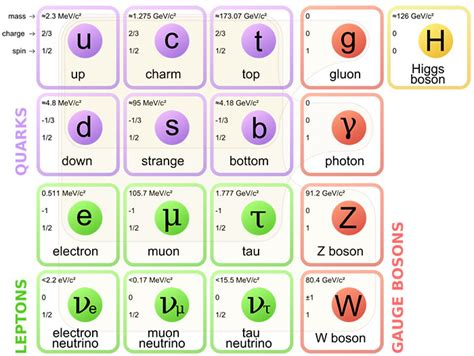
\includegraphics[width=0.5\textwidth]{standard_model.png}
When looking at phenomena outside our earth the astronomer will turn to
electromagnetic radiation, but he's missing out on a big part of the full
picture. Not only do interesting events emit photons but also muons, nuclei,
gravitational waves,... All kinds of particles which might also be of interest,
that's where the astroparticle physicist comes in.

Of all these particles there is one particle which has properties we're quite
interested in: the neutrino.  Neutrinos don't have any charge, meaning that
they are not deflected by magnetic fields. Also neutrinos interact very weakly,
because of this they are often called “ghost” particles; on average 100
trillion neutrinos pass through your body per second, none of them having any
effect.  You'd even need a light year of lead to give you just a 50\% chance of
stopping a neutrino.
These properties makes them ideal messenger particles as, when we detect a neutrino
and it's arrival direction, we can be quite sure it came to our detector unhindered
from a far away event in the exact same direction.
Neutrinos can serve as unique clues
about what’s happening elsewhere in the universe including the cosmic
collisions, galaxies, supernovae, Gamma-ray bursts (GRBs),... where they are created.

\section{Discovery}
When researching $\beta^-$ decay, the decay of a neutron, researcher
detected a proton and an electron coming from the neutron. However
on closer inspection it became apparent that energy was lost
somewhere in violation with the conservation law of energy, and
angular momentum wasn't conserved.  The solution postulated by
Wolfgang Pauli was to introduce a new, really hard to detect
particle with no charge and a very small mass: the neutrino.  The neutrino comes in three flavours:
electron, muon and tau neutrinos, each corresponding to their respective lepton denoted as
\begin{equation}
	\nu_e \quad \nu_\mu \quad \nu_\tau
\end{equation}
and each also having an anti-particle.
\begin{equation}
	\bar{\nu}_e \quad \bar{\nu}_\mu \quad \bar{\nu}_\tau
\end{equation}

Now with the introduction of the neutrino the full $\beta^-$ decay
becomes
\begin{equation}
	n \rightarrow p^+ + e^- + \nu_e
\end{equation}
The inverse can then also be used to detect neutrinos:
\begin{equation}
	n \rightarrow p^+ + e^- + \nu_e
\end{equation}
Which is called beta capture and was first experimentally detected in 1956
\cite{BetaCapture} also making it the first experimental detection of a
neutrino.
\section{Charged and neutral currents}
As with the strong and electromagnetic interaction whom interact via gluons
and photons respectively, the weak interaction which is the primary way
neutrinos interact, is also mediated by the exchange of elementary spin-1
bosons.  Namely the charged bosons $W^+$ and $W^-$ and the neutral $Z^0$ boson.
Contrary to the gluons and photons however, these bosons are very massive:
\begin{equation}
  M_W = 80.40\text{ GeV }\quad M_Z = 91.19\text{ GeV }
\end{equation}
Following general arguments, it can be derived that the
range of any force is given by the compton wavelength of the particles transmitting it\cite{martin2017particle},
as the compton wavelenght is given by 
\begin{equation}
  \lambda = \frac{h}{mc}
\end{equation}
The very large mass of the "force carriers" imply a very short-range
interaction, in the order of $10^{-3}$fm and can even be treated as a
zero-range interaction at low energies.

These bosons can couple to leptons (e.g neutrinos, electrons, tauons and muons)
but also to quarks, if they couple via the charged bosons then the coupling process
is called a \textit{charged current} reaction and if they couple via the $Z^0$ boson
than the process is called a \textit{neutral-current} interaction.

A simple interaction is sketched below
\begin{equation}
  \mu^- \rightarrow e^- + \bar{\nu}_e + \nu_\mu
\end{equation}
here the muon decays via a charged current reaction, note that lepton number needs to be conserved.
This means that, as on the left side of the reaction we have $\ell_\mu = 1$ and $\ell_e = 0$ this needs
to be the case on the right side. The lepton number is conserved as a muon neutrino counts for $\ell_\mu = 1$
and an electron anti-neutrino counts for $\ell_e = -1$
\section{Neutrino sources}
As shown in figure \ref{figure:Neutrino fluxes} there are various kinds of
neutrino sources, we'll discuss these one by one in order leaving out the
reactor anti-neutrinos and the terrestrial anti-neutrinos as we're only
interested in neutrinos of astrophysical nature.
\begin{figure}
	\centering
	\copyrightbox[r]{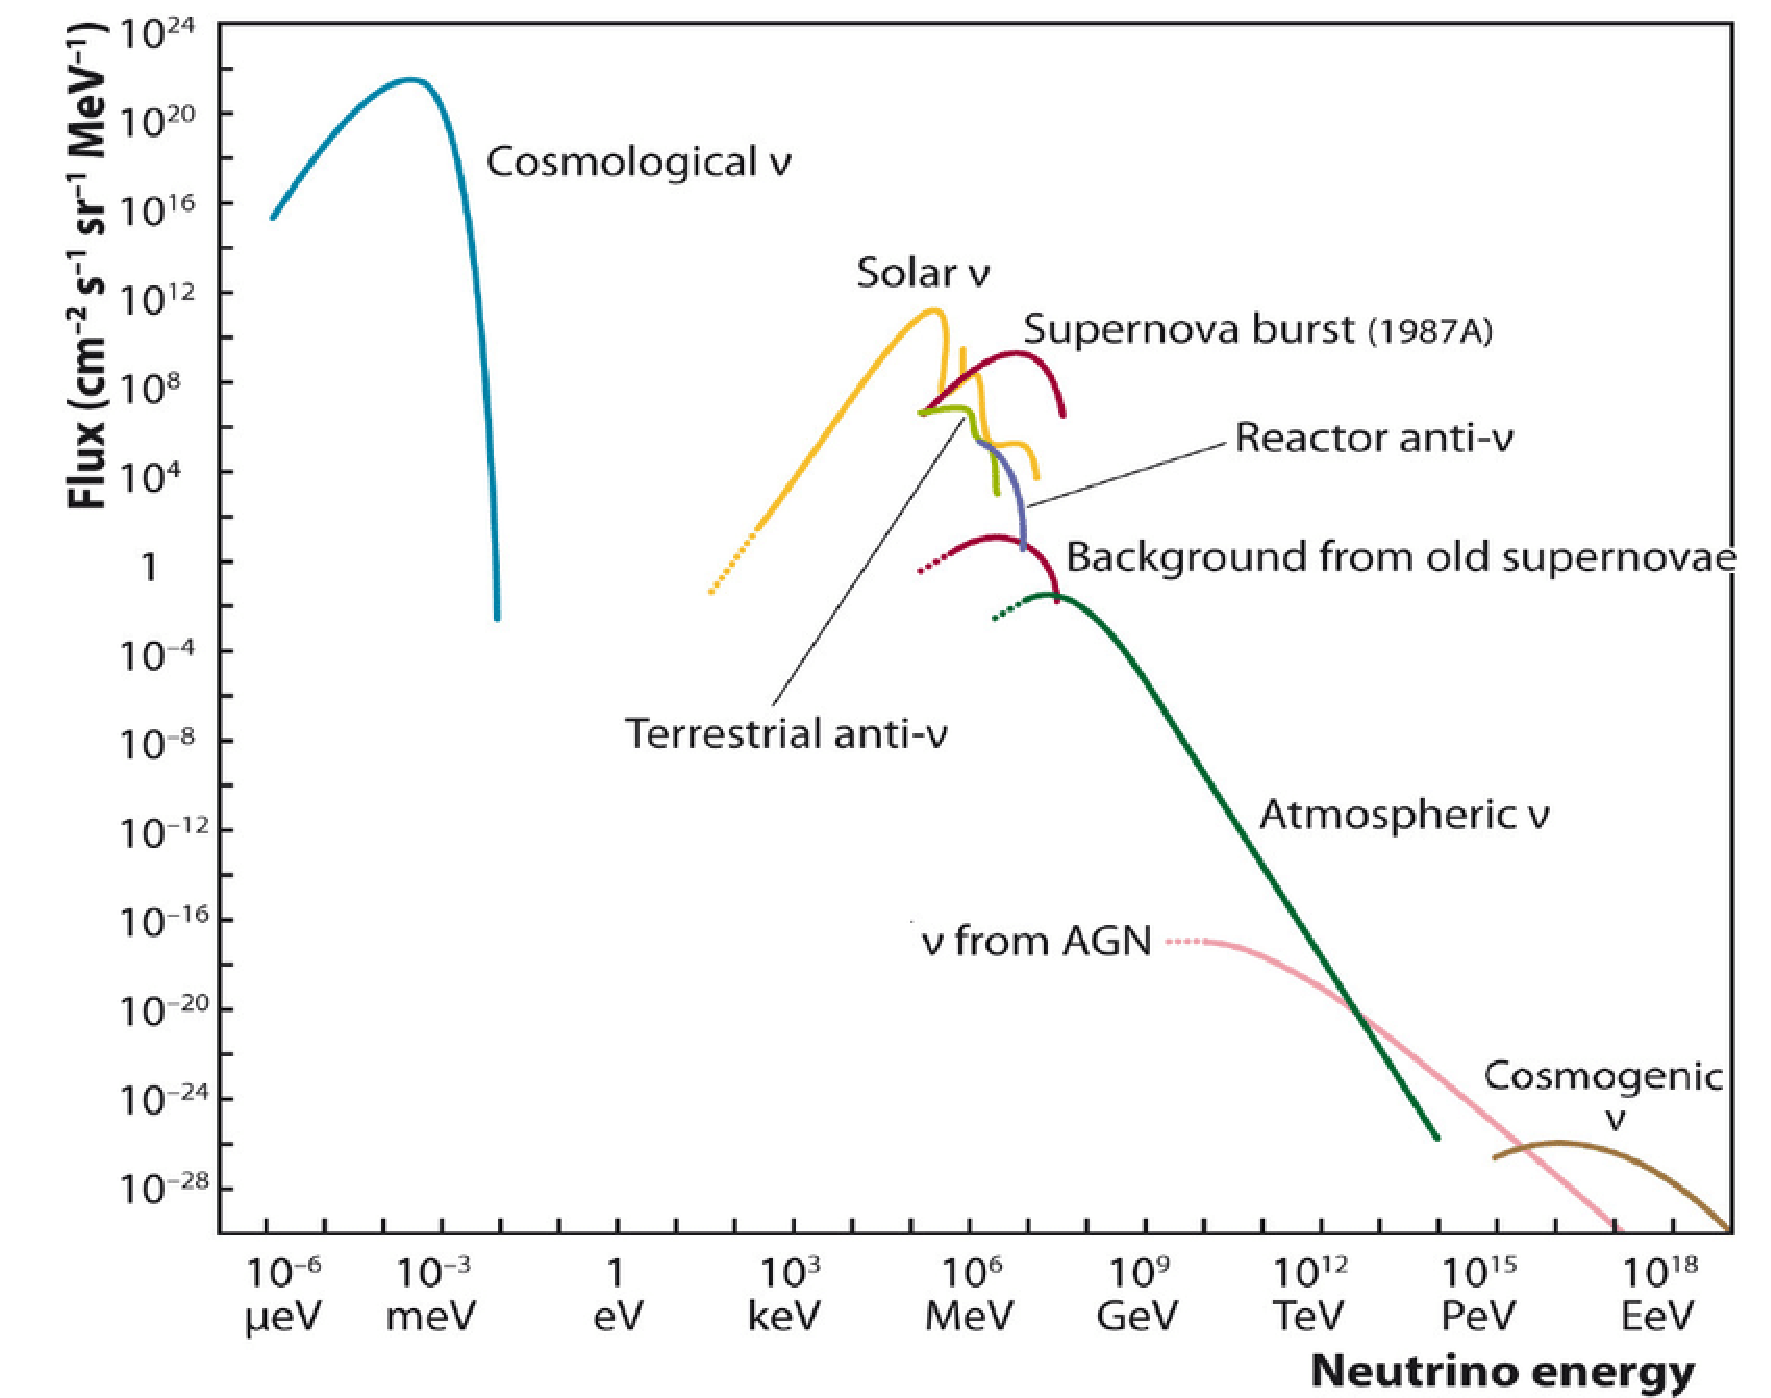
\includegraphics[height = 0.5\textwidth]{neutrinofluxes.pdf}}{\textcopyright Abhik Jash, Studies on the Physics of Resistive Plate Chambers in Relation to the INO Experiment}
	\caption{Predicted neutrino flux for various sources both natural and man-made}
	\label{figure:Neutrino fluxes}
\end{figure}
\subsection{Cosmological/Primordial neutrinos}
The first source of neutrinos we'll talk about is the one in blue to the left of the figure
termed the \textit{Cosmological neutrinos}: 
the neutrino version of the CMB.
To understand this source we'll have to go back all the way to just after the big bang:
The very early universe was hot and dense. As a result, interactions among particles
occurred much more frequently than they do today. As an example, a photon today
can travel across the observable universe without deflection or capture, so it has a
mean free path greater than $10^{26}$ m. When the universe was 1 second old, though, 
the mean free path of a photon was about the size of an atom. Thus in
the time it took the universe to expand by a factor of 2, a given photon interacted
many, many times. These multiple interactions kept the consitituents in the universe
in thermal equilibrium. But as the universe expanded there were times when reactions could
not proceed rapidly enough to maintain equilibrium conditions, these particles then fall out
of thermal equilibrium. This falling out of equilibrium is termed \textit{decoupling}.
And we're interested in when neutrinos decoupled.
Neutrinos were kept in equilibrium through the interaction 
\begin{equation}
	\nu e \leftrightarrow \nu e
\end{equation}
up until the universe cooled down to about 1MeV when they decoupled.
To estimate the temperature of the neutrinos who decoupled at the start of the universe, 
we can take a look at conservation of entropy \cite{Dodelson} from which we'll find that
the temperatures are related by:
\begin{equation}
	T_\nu = \left(\frac{4}{11}\right)^{1/3}T_\gamma
\end{equation}
Note that they decoupled before the photons making them lower in temperature.
As $T_\gamma$ is the CMB temperature which, nowadays, is measured to be around
2.7K or $2.3\times10^{-4}$MeV. This would imply $T_\nu = 1.66\times 10^{-4}$MeV which
is rougly where the peak flux is located.  these primordial neutrinos are thus very
low in energy.
\subsection{Solar neutrinos}
The sun fuses elements to release energy and thus keeping itself from collapsing in 
on itself, with most of the various ways particles get fused, neutrinos get released as 
is shown in figure \ref{fig:SunFusion} where the neutrinos are electron neutrinos.
\begin{figure}
	\centering
	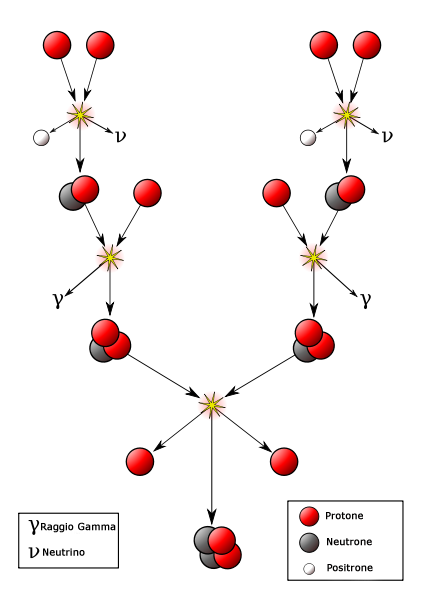
\includegraphics[width=0.4\textwidth]{figures/SunFusion.png}
	\caption{illustration of the full fusion cycle in the sun}
	\label{fig:SunFusion}
\end{figure}
Now with this and some information about the sun like the pressure and mass,
the \textit{standard solar model} was made. This model predicted a certain
amount of electron neutrinos to be hitting the earth from the previously mentioned
thermonuclear fusion, it was however 3 times higher than the observed amount of
electron neutrinos back at our planet. This led to a little bit of hysteria as this could've meant
that the sun was dying and we'd see the aftermath only in a couple of years.
Through various experiments however, it became apparent that this was due to
the different kinds of neutrinos oscillating into each other on their way to
earth, i.e 2/3 of the original electron neutrinos had oscillated into mu and
tau neutrinos. But for them to oscillate into eachother, they not
only require mass but each flavor also should have a different mass as can be seen
from an example 2D approximation to the transition probability\cite{Bellini_2014}:
\begin{equation}
	P(\nu_e\rightarrow\nu_\mu) = |\braket{\nu_\mu|\psi(L,T)}|^2 = c_\mu c_\mu^* = \sin ^2(2 \theta) \sin ^2\left(\frac{\Delta \phi_{12}}{2}\right)
\end{equation}
with
\begin{equation}
	\Delta \phi_{12} \approx \frac{m_1^2 - m_2^2}{2p}L
\end{equation}
In full generality (3D):
\begin{equation}
	\ket{\nu_\alpha} = \sum_iU_{\alpha i} \ket{\nu_i}
\end{equation}
With $U_{\alpha i}$ the Pontecorvo-Maki-Nakagawa-Sakata (PMNS) matrix.  This
phenomenon has been experimentally verified e.g through the descrepency from
the observed and expected neutrino events coming from a nuclear reactor \cite{Eguchi_2003}.
\subsection{Supernovae}
\label{sec:supernovae}
A star starts its life as a ball of pure hydrogen. At the core, due to the
gravitational pressure of the outside plasma, fusion of hydrogen into deuterium
and helium happens. Thus converting mass into energy. The pressure of this energy
counteracts the pressure of gravity and the star is stable.

When the hydrogen at the core runs out no more hydrogen can be fused. For stars
with masses between $8M_\odot$ and $30M_\odot$ ($M_\odot$ being the mass of the sun)
the fusion of heavier elements starts, this can't keep going on however as at
some point the star starts to form the most stable element: iron. 
\begin{figure}[!ht]
	\centering
	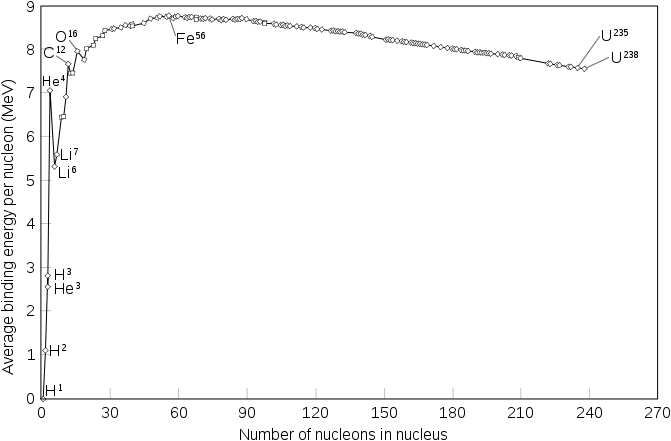
\includegraphics[width=0.5\textwidth]{Binding_energy_curve.png}
	\caption{Energy curve showing that iron is the most stable atom}
	\label{fig:BindingEnergyCurve}
\end{figure}
It costs energy
to both make lighter elements than iron and heavier ones as can be seen on
figure \label{fig:BindingEnergyCurve}.  As the iron core builds up the outside
pressure from the core starts to decrease as no new energy is released. This
goes on until  the treshold of an iron core with a mass of 1.4$M_\odot$ known
as the Chandrasekhar limit is reached and the the inwards pressure becomes too
large compared to the outwards pressure, making the electrons surrounding the
iron core fuse with the protons (uud), creating neutrons (udd) and neutrinos,
diagramatically shown in figure
\ref{fig:CoreFusion}.
\begin{figure}
	\centering
	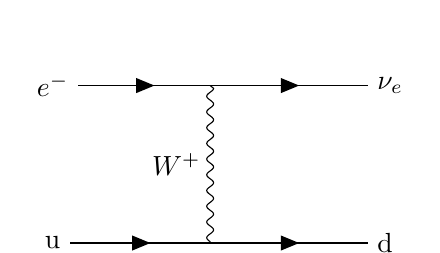
\begin{tikzpicture}
	\begin{feynman}
	\vertex (a0){u};
	\vertex[right=2cm of a0] (am) ;
	\vertex[right=2cm of am] (a1) {d};
	\vertex[above=2cm of am] (bm);
	\vertex[above=2cm of a0] (b0){$e^-$};
	\vertex[right=2cm of bm] (b1){$\nu_e$};
	\diagram* {
		{[edges=fermion]
			(a0) -- (am) -- (a1)
		},
		{[edges=fermion]
			(b0) -- (bm) -- (b1)
		},
		{[edges=boson,edge label=$W^+$]
			(am) -- (bm)
		}
	};
	\end{feynman}
	\end{tikzpicture}
	\caption{fusion of protons with surrounding electrons into neutrons via the weak force}
	\label{fig:CoreFusion}
\end{figure}\\
This last part happens in a split second as the collapse goes at 25\% the speed
of light, creating a very dense neutron star (3000km in diameter iron core to
30km in diameter neutron star) and up to $10^{52}$ ultra-relativistic
neutrinos, carrying up to 99\%\footnote{$\approx$1\% is released as kinetic energy, only 0.001\% as
electromagnetic radiation} of the released energy
\cite{Melson_2015}. As the density has suddenly increased so much
there's a huge distance of pure vaccuum between the plasma outer layer and the
(now) neutron star, this plasma starts free-falling inwards, also at 25\% the
speed of light whilst the neutrinos carrying tremendous amounts of energy start
going outwards from the neutron stars core.

The neutrinos then collide with the plasma resulting in what we observe as a
"supernova", wrongly thought of by Kepler as being a "new (nova) star" rather
being a violent death of an old star.

This is quite unexpected as neutrinos rarely interact, it's only as the
incoming plasma is so dense and due to the tremendous amount of neutrinos that
collissions happen at all. Some, however, escape and will be visible on earth
in our neutrino detectors $\approx$ 18h before the light escapes the exploding
star.

Neutrino observatories are thus also useful to know where to point our various
telescopes before the supernova is actually visible in the night sky.
\subsection{Background from old supernovae}
Also termed the \textit{diffuse supernova neutrino background} (DSNB), as the
universe is quite old various supernovae have happened over it's lifetime, each generating
a lot of neutrinos as was discussed in section \ref{sec:supernovae}. 
This is postulated to have generated a continuous neutrino background.
\subsection{Atmospheric neutrinos}
\label{sec:AtmosphericNeutrinos}
Before we can talk about atmospheric neutrinos it's necessary to discuss \textit{cosmic rays}.
Cosmic rays are ionized nuclei of which 90\% are protons, 9\% are alpha particles and
the rest are heavier nuclei. Almost all of them originate from outside the solar system but
from within our galaxy, the few particles that do come from our solar system can be temporally
linked to violent events on the sun. In contrast to this the particles coming from outside
our solar system show an anti-correlation with the sun as they can more easily reach the earth
if solar activity is low.
It has been observed that they roughly follow a power-law spectrum 
$N \propto E^{-\gamma}$ \cite{gaisser_engel_resconi_2016}.

Cosmic rays hit the Earth's atmosphere at a rate of about 1000 per square meter
per second and interact with atomic nuclei in the Earth's atmosphere, creating
showers of particles, many of which are unstable and produce neutrinos when
they decay, these neutrinos are what's called \textit{Atmospheric neutrinos}.
Most notably neutrinos can be produced together with muons in the two-body
decays of charged pions and kaons wherever these hadronic interactions occur.
The most important production channels and their branching ratios for neutrinos
are:
\begin{align}
	\pi^\pm &\rightarrow \mu^\pm + \nu_\mu(\bar{\nu}_\mu) (\sim 100\%)\\
	K^\pm &\rightarrow \mu^\pm + \nu_\mu(\bar{\nu}_\mu) (\sim 63.5\%)
\end{align}
Neutrinos are subsequently also produced when these muons decay:
\begin{equation}
	\mu^\pm \rightarrow e^\pm + \nu_e(\bar{\nu}_e) + \bar{\nu}_\mu(\nu_\mu)
\end{equation}
which is a process mainly happening at low energies in the atmosphere.  The
atmospheric neutrino spectrum shown in figure \ref{figure:Neutrino
fluxes} roughly follows a power spectrum as the cosmic ray flux follows a power
spectrum but the correspondence isn't one-to-one as, due to the difference in
kinematics, the contribution from kaons to neutrinos is significantly more
important than to muons, especially at high energies.

\subsection{neutrinos from AGNs}
An AGN (active galactic nucleus) is deemed to be the reason why several abnormal galaxies exist with
an extra bright (and mostly variable) light source in their core which even the biggest of telescopes
can't spatially discern. The general concensus is that this phenomenon is caused by one particular
kind of object: a supermassive black hole (a black hole with a mass of at least 105M$_\odot$) surrounded with
a close torus of dust and gas.
This torus of gas is called an \textit{accretion disc} and is an enormous source of energy. The conversion
of potential energy of the incoming gas to highly energetic radiation is a very complex physical process
with which we have to account for various factors like gravitational instabilities, magnetic fields, hydrodynamical
turbulence,... And thus produces a spectrum that's quite complex.
It would appear that the luminocity of an AGN would increase indefinitely with incoming mass, but this process is 
limited: if too much matter accretes on the black hole the radiative pressure becomes too massive and the 
matter on the disc gets blown away, this phenomenon is termed a \textit{black hole outburst}.

The emission of high energy neutrinos from AGNs rests solely on the premise
that relativistic protons of sufficiently high energy and energy density in the
AGN's accretion disc will be present \cite{NASANeutrinos} as they may interact
to create e.g pions whom decay into neutrinos. A direct consequence of the occurence of these
relativistic protons is the production of $\gamma$-rays of similar energies to
those of the neutrinos, thus high energy neutrino- and $\gamma$-ray astronomy are
closely related.  However, even though $\gamma$-ray photons can be produced
even in the absence of relativistic protons (e.g via high energy electrons),
neutrinos can not.  Thus the detection of these high-energy neutrinos (which
might have already been detected \cite{AGNNeutrino}) will provide unique
information about the workings of AGNs.
As these ultra high energy neutrinos get produced near the source (the AGN)
they are what's called \textit{astrophysical neutrinos}

\subsection{Cosmogenic neutrinos}
In contrast to the previous source of UHE neutrinos which was generated at the
source, called \textit{astrophysical neutrinos} we'll now talk about UHE
neutrinos whom are generated through the interaction of ultra-high energy
cosmic rays during propagation with the cosmic microwave or other photon
backgrounds termed \textit{cosmogenic neutrinos}.  The mechanism by which these
get created is quite simple, if a proton has sufficiently high energy the cross
section to interact with CMB (Cosmic Microwave Background) photons becomes
non-negligable.  These protons can scatter off the photons to resonantly
produce a $\Delta^+$ baryon.  This resonance has enough mass to dominantly
decay to a pion and a nucleon:
\begin{align}
	\Delta^+ &\rightarrow \pi^0 + p \ \ (2/3)\\
	\Delta^+ &\rightarrow \pi^+ + n \ (1/3)
\end{align}
Of which the charged pion decays to neutrinos as previously mentioned in 
\ref{sec:AtmosphericNeutrinos}.
\subsection{How do they fit into the full detector spectrum?}
The origin of the most energetic cosmic rays is still not conclusively
identified. One approach to solving this problem is \textit{multi-messenger
astrophysics}, where several types of cosmic particles are used to identify the
sources of these ultra-high energy cosmic rays (UHECRs). E.g we simultaneously
measure gravitational waves with the Einstein telescope, neutrinos with RNO-G,
photons with various telescopes and muons with a muon detector.
\newpage
\chapter{Radio neutrino detection}
Neutrinos on their own aren't detectable, unlike say protons we can't expect
them to produce brehmsstrallung or any other kind of directly observable
radiation as they aren't charged and thus don't couple to photons. We'll need
to convert them to charged particles first which then can generate some kind of
detectable signal.  

To this end we'll need a big volume in which they can interact to produce
charged particles, we'll be choosing ice for this.  Even though there are a lot
of volumes such as the water or rock the ice has a few particular properties
which make it more usable:
\begin{itemize}
  \item contrary to some kind of sediment, ice is mostly see-through for electromagnetic radiation but it's still possible
    to differentiate between neutrino signals and other particles
  \item contrary to water as a medium which is used e.g in the Super-Kamiokande detector\cite{SuperKamio}, ice
    was naturally formed and it isn't needed to construct some kind of dome
\end{itemize}
\section{Neutrino interactions in ice}
As neutrinos propagate through ice they can interact weakly with the nuclei.
The main mechanisms of interaction is via charged- and neutral
currents\cite{NuRadioMc} as is also depicted in figure
\ref{fig:NeutrinoNucleusInteraction}.
\begin{figure}[h!]
	\begin{minipage}{\textwidth}
		\begin{minipage}{0.49\textwidth}
			\centering
			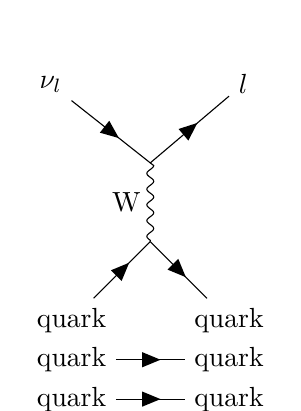
\begin{tikzpicture}
				\begin{feynman}
					\vertex (a0) {quark};
					\vertex[above=0.5cm of a0] (a1) {quark};
					\vertex[above=0.5cm of a1] (a2) {quark};
					\vertex[right=2cm of a0] (b0) {quark};
					\vertex[right=2cm of a1] (b1) {quark};
					\vertex[right=2cm of a2] (b2) {quark};
					\vertex[right=1.0cm of a2] (am);
					\vertex[above=1cm of am] (c0);
					\vertex[above=1cm of c0] (c1);
					\vertex[above=1cm of c1] (cm);
					\vertex[left=1cm of cm] (a3) {$\nu_l$};
					\vertex[right=1cm of cm] (b3) {$l$};
					\diagram* {
						{[edges=fermion]
							(a0) -- (b0)
						},
						{[edges=fermion]
							(a1) -- (b1)
						},
						{[edges=fermion]
							(a2) -- (c0) -- (b2)
						},
						{[edges=fermion]
							(a3) -- (c1) -- (b3)
						},
						{[edges=boson, edge label=W]
							(c0) -- (c1)
						},
					};
				\end{feynman}
			\end{tikzpicture}
		\end{minipage}
		\begin{minipage}{0.49\textwidth}
			\centering
			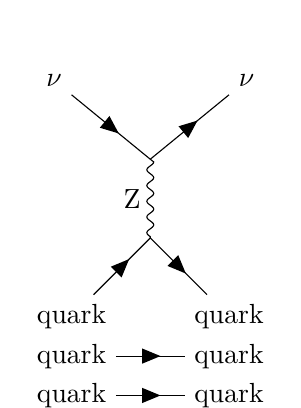
\begin{tikzpicture}
				\begin{feynman}
					\vertex (a0) {quark};
					\vertex[above=0.5cm of a0] (a1) {quark};
					\vertex[above=0.5cm of a1] (a2) {quark};
					\vertex[right=2cm of a0] (b0) {quark};
					\vertex[right=2cm of a1] (b1) {quark};
					\vertex[right=2cm of a2] (b2) {quark};
					\vertex[right=1.0cm of a2] (am);
					\vertex[above=1cm of am] (c0);
					\vertex[above=1cm of c0] (c1);
					\vertex[above=1cm of c1] (cm);
					\vertex[left=1cm of cm] (a3) {$\nu$};
					\vertex[right=1cm of cm] (b3) {$\nu$};
					\diagram* {
						{[edges=fermion]
							(a0) -- (b0)
						},
						{[edges=fermion]
							(a1) -- (b1)
						},
						{[edges=fermion]
							(a2) -- (c0) -- (b2)
						},
						{[edges=fermion]
							(a3) -- (c1) -- (b3)
						},
						{[edges=boson, edge label=Z]
							(c0) -- (c1)
						},
					};
				\end{feynman}
			\end{tikzpicture}
		\end{minipage}
	\end{minipage}
	\caption{Most prominent ways of neutrino-nucleus interaction}
	\label{fig:NeutrinoNucleusInteraction}
\end{figure}\\
With the produced leptons in the W boson mediated interaction being either electrons,
resulting in an electromagnetic shower, muons wich typically go undetected as they live
too long or
tauons wich will decay via
\begin{equation}
	\tau^- \rightarrow e^- + \bar{\nu}_e + \nu_\tau
\end{equation}
or, less ideally
\begin{equation}
	\tau^- \rightarrow \mu^- + \bar{\nu}_\mu + \nu_\tau
\end{equation}
In both of the possible interactions (W or Z exchange) the resulting nucleus
will result in an hadronic shower, for the neutral current interaction (mediated
by the Z boson) the fraction of the neutrino energy that gets transferred to
the nucleon is described by the inelasticity $y$ and is heavily shifted towards
small values of $y$\cite{elasticity_y}. This causes a big, irreducable
uncertainty when trying to estimate the original neutrino energy from these
kinds of events.  With the charged current interaction (mediated by the $W^\pm$
bosons) this isn't a problem however as the full neutrino energy ends up in the
resulting cascades.
\section{Askaryan effect}
\label{sec:Askaryan}
For a particle shower to emit strong radio signals, two conditions have to be met:
\begin{itemize}
	\item There needs to be a separation of positive and negative charges in the shower front 
	\item The signals produced over the length of the shower profile need to overlap coherently.
\end{itemize}
The \textit{Askaryan} \cite{Askaryan} effect, which is responsible for the
production of Askaryan radiation describes the effect at radio frequencies
which abides by both of these conditions.  In general it's a quite difficult
effect but we'll give a crude overview.  The previously described interactions
of the neutrinos with nuclei create a shower of secondary charged particles
containing a charge anisotropy.  This charge imbalance is a result of medium
electrons either Compton scattering into the advancing shower or annihilating
with shower positrons.  In the end you have a moving charge anisotropy,
propagating faster than the speed of light in the medium, creating Cherenkov
radiation.  

Cherenkov radiation is like the electromagnetic equivalent of a sonic boom, a
sonic boom happens when something goes faster than the speed of sound in the
medium; A particle emits Cherenkov radiation if it goes faster than the speed
of light in the medium.  Choosing the particle trajectory to lie along the z
axis an approximate equation can be found\cite{jackson1998classical} for
$\frac{\text{d}^2 \mathscr{J}}{\text{d}\omega \text{d}\Omega}$, which is the energy
radiated per elementary unit solid angle and per elementary unit frequency
interval:
\begin{equation}
	\frac{\text{d}^2 \mathscr{J}(\omega)}{\text{d} \omega \text{d} \Omega} = \frac{q^2}{4\pi}\sqrt{\frac{\mu}{\epsilon}}\beta^2\omega^2\delta^2[\omega(1-\beta \mathbf{e}_r\cdot\mathbf{e}_z)]|\mathbf{e}_r\times\mathbf{e}_z|^2 \label{equation: 4.128 in elektromagnetisme}
\end{equation}
Now we can re-write this equation in spherical coordinates, which gives $1-\beta \mathbf{e}_r\cdot\mathbf{e}_z = 1-\beta\cos(\theta_c)$ in the delta function. We thus only expect radiation if
\begin{equation}
\cos(\theta_c) = \frac{1}{\beta} = \frac{c'}{u} = \frac{c}{n}\cdot\frac{1}{u}
\end{equation}
With u the local speed of light in the medium and n the index of refraction, an optical
property of a medium which we'll later on thoroughly discuss.
If $u>\frac{c}{n}$, Cherenkov radiation will
be emitted along a cone surface with half angle $\frac{\pi}{2}-\theta_c$ as
illustrated in figure \ref{figure: Cherenkov illustratie}. Integrating equation
\ref{equation: 4.128 in elektromagnetisme} over the solid angle and formally
dividing by the time interval we get:
\begin{equation}
	\frac{\text{d}^2\mathscr{J}}{\text{d}\omega \text{d}t} = \frac{q^2}{4\pi}\sqrt{\frac{\mu}{\epsilon}}\beta\omega\left(1-\frac{1}{\beta^2}\right)	
\end{equation}
We see that the energy is proportional to $\omega$, so we expect that most
radiation will be emitted "in blue" with a cut-off frequency above which the
equation $\cos\theta = 1/(n\beta)$ can no longer be satisfied, this "in blue"
characteristic is responsible for the blue glow seen in nuclear reactors as
seen in figure \ref{figure: Cherenkov reactor} .  For ice the index of
refraction is roughly 1.78 in deep ice, so we expect an ultra-relativistic
particle to produce the most radiation at around 56° opening as 
\begin{equation}
	\cos(\theta_c) \approx \frac{1}{n} \implies \cos^{-1}\left(\frac{1}{1.78}\right)\approx 56\text{°}
\end{equation}
\begin{figure}
\centering
\begin{minipage}{0.45\textwidth}
	\centering
	\copyrightbox[r]{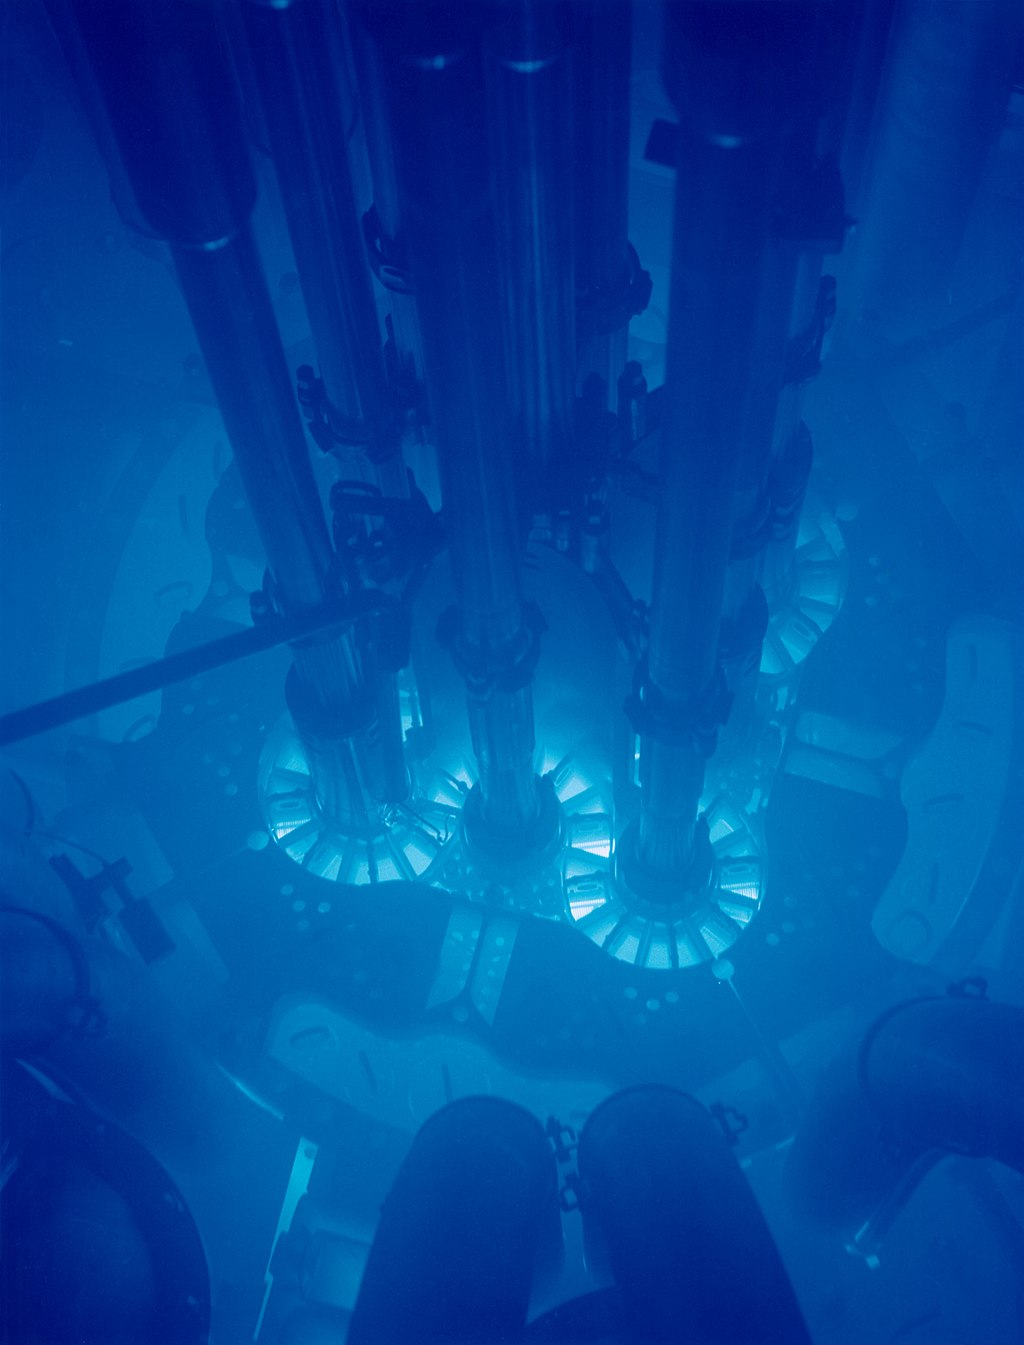
\includegraphics[height = 0.8\textwidth]{Cherenkov-reactor.jpg}}{\textcopyright Argonne National Laboratory\\Advanced Test Reactor core, Idaho National Laboratory}
	\caption{Cherenkov radiation in a nuclear reactor}
	\label{figure: Cherenkov reactor}
\end{minipage}
\hspace{0.05\textwidth}
\begin{minipage}{0.45\textwidth}
	\centering
	\copyrightbox[r]{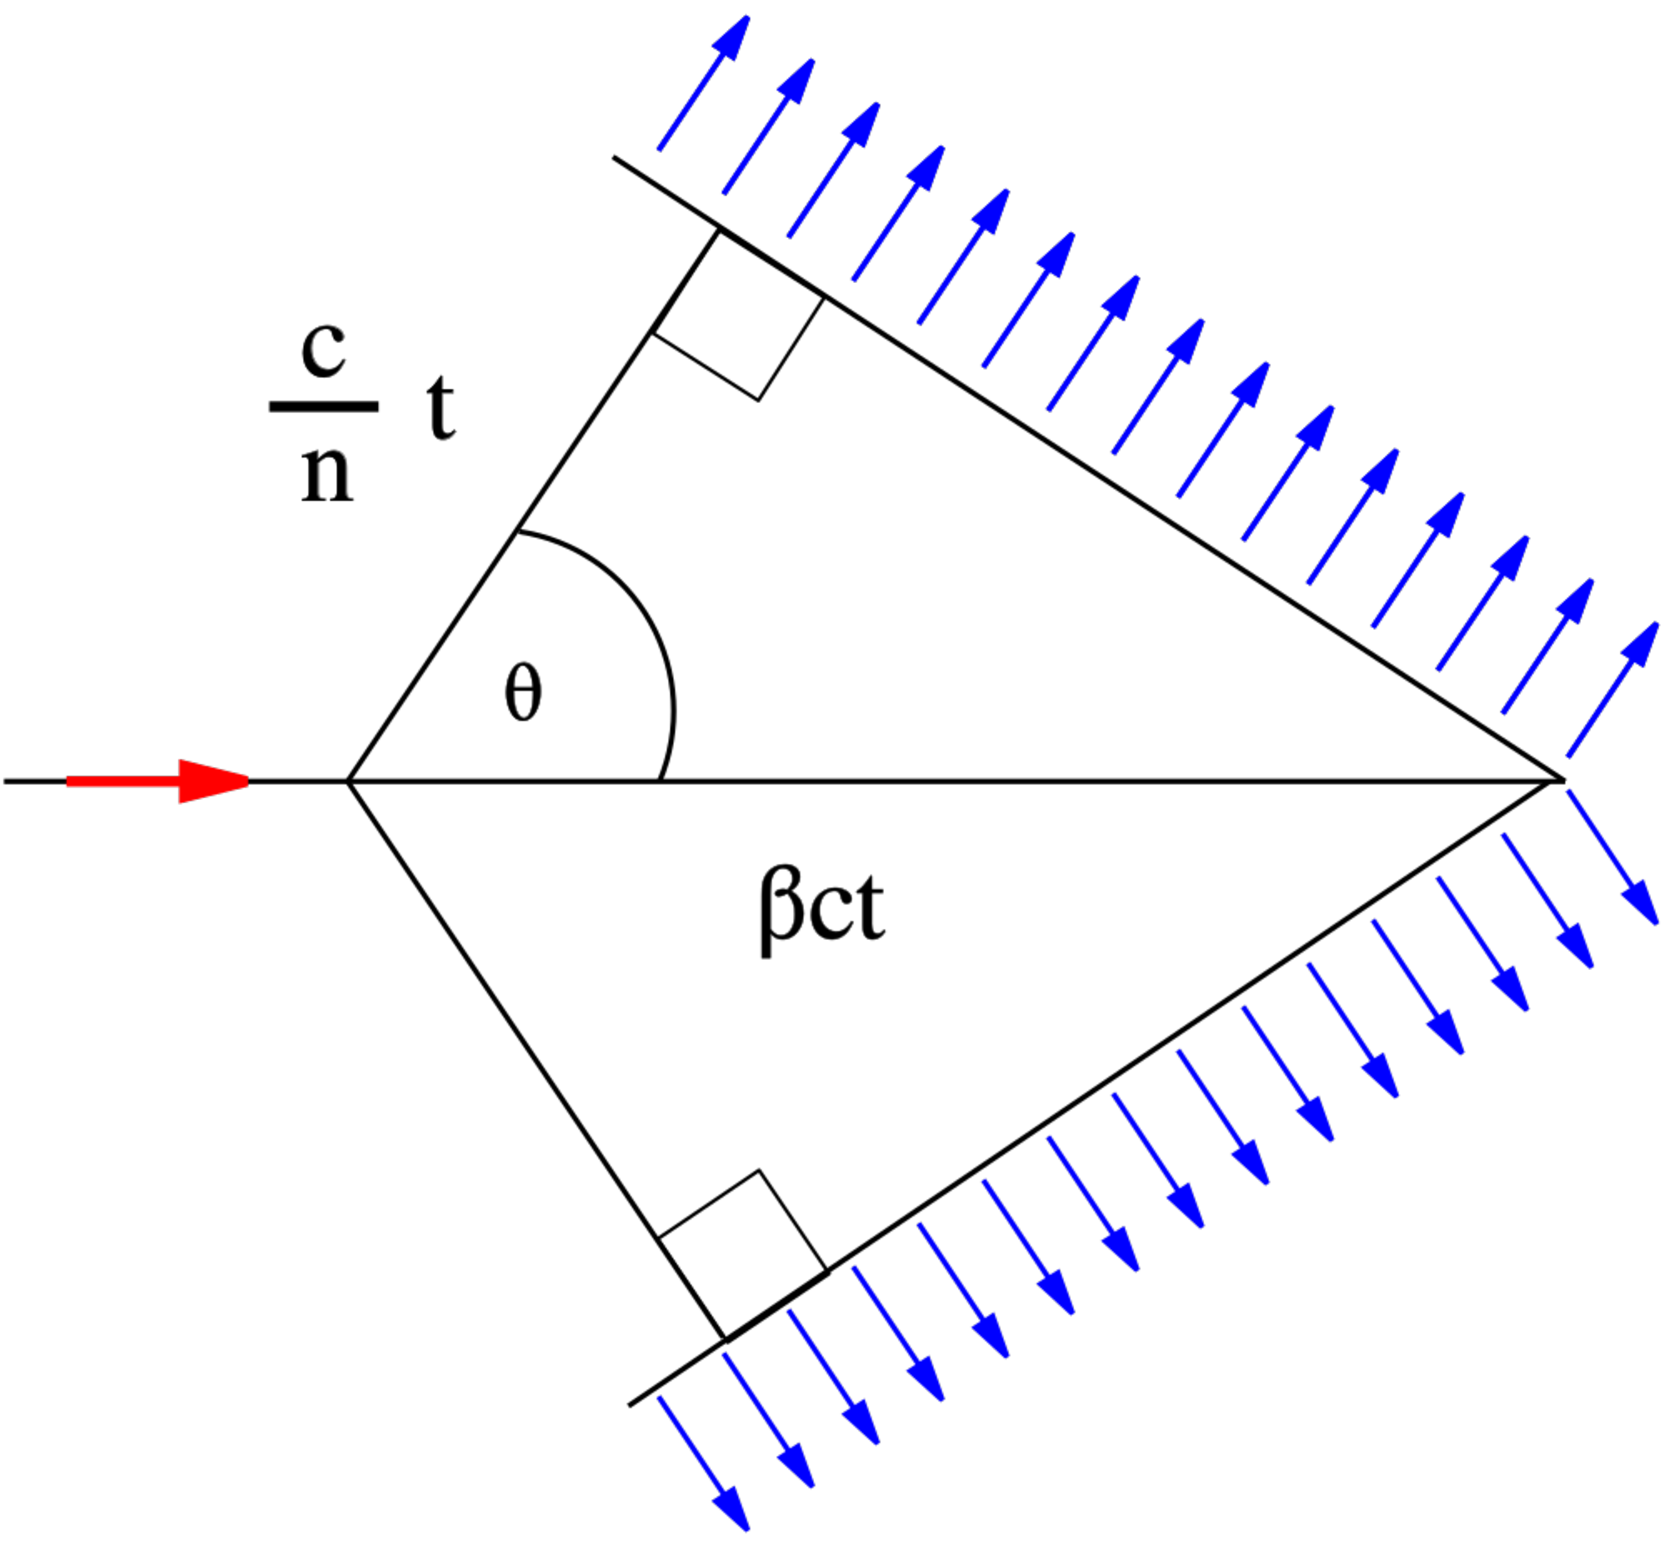
\includegraphics[height = 0.8\textwidth]{Cherenkov.pdf}}{\textcopyright Arpad Horvath}
	\caption{Diagrammatic representation of Cherenkov radiation}
	\label{figure: Cherenkov illustratie}
\end{minipage}
\end{figure}
Of course this is just an estimate, as the actual index of refraction is depth-dependent which
we'll get to in section \ref{section:Ice Model}.
Now this explains how the signals get generated but logically, from only knowing this
we'd expect radio waves to almost be non-existent 
due to the "in blue" nature of Cherenkov radiation. 

This isn't the full story however as we'll need to talk about coherent overlap
to fully understand the Askaryan effect. This can be intuitively explained as
follows: generally the shower is of length
$\mathcal{O}$(10cm)\cite{Huege_2017}, over this length the radiation gets
emitted, most frequencies decoherently interfering, but radio waves with wavelengths of 
$\approx$ 10cm coherently interfere, and it's these waves we then wish to detect.


The generated electromagnetic radiation is polarized perpendicular to the
cherenkov cone, this can be useful to discern between different cherenkov cones whom,
timely, would generate the same response. This concept is illustrated below in 2D where
two neutrinos from different directions would generate the same signal in the detector.

\begin{figure}[h!]
	\centering
	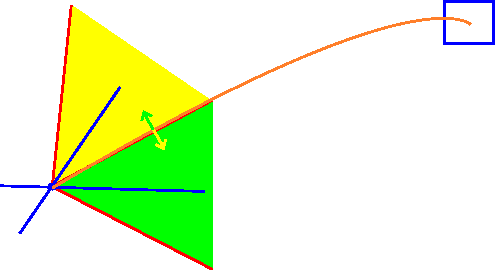
\includegraphics[width=0.5\textwidth]{illu_polarization.pdf}
\end{figure}

If the detector has a way to differentiate between polarization however, there would be no
doubt where the neutrino originated from as the one producing the yellow cherenkov cone
would have a downwards polarization and the one producing a green cherenkov cone would have
an upwards polarization, note that in 3D infinite different cherenkov cones could generate
the same timely signal (think of rotating the cone around a line on the cone) so both vertical
and horizontal polarization information is needed.


\section{RNO-G}
Both cosmic ray and neutrino detectors face the same main problem at the
highest energies: the steeply falling flux (as was previously seen in figure
\ref{figure:Neutrino fluxes}) requires large effective areas, which leads to
the construction of neutrino detectors with volumes on the cubic kilometer
scale like IceCube\cite{IceCubeTechnical} which works on the principle of
detection neutrinos with visible light.  But even IceCube has it's limitations,
it's still too small to observe neutrino events above the 10 PeV
scale\cite{IceCubeGen2}, that's why a new detector was needed which was even
bigger and able to observe Cosmogenic neutrinos.  We could just make IceCube
bigger but this would cost a lot of money as the individual detectors need to
be spaced closely as the attenuation length is quite short for light in the
visible spectrum propagating through ice.  

The proposed solution was to work with radiowave detectors, leveraging the
previously discussed Askaryan effect (see section \ref{sec:Askaryan}).  Besides
the advantage radiowaves have due to their abundance, they can also propagate
way further in ice than visible light making it possible to space the
individual detectors further apart. The proposed location was Greenland, an
island country in North America and part of the Kingdom of Denmark which has
large ice sheets.
\begin{figure}
  \centering
  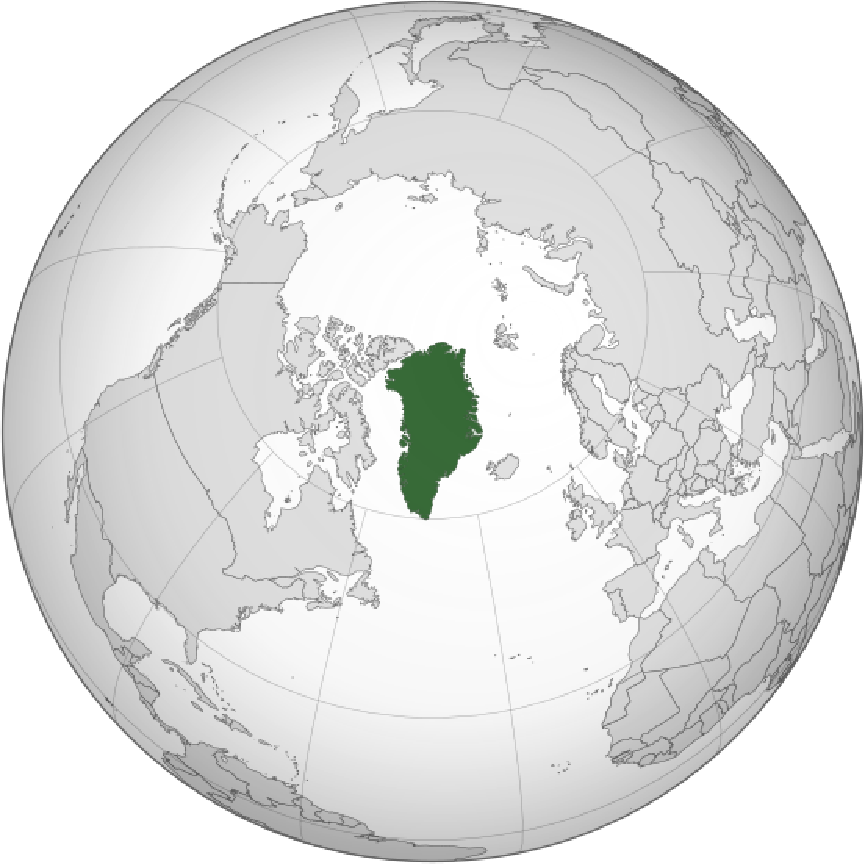
\includegraphics[width=0.5\textwidth]{figures/GreenlandOP.pdf}
  \caption{orthographic projection of Greenland with the red star representing the approximate RNO-G location}
  \label{fig:GreenlandOP}
\end{figure}
The proposal for RNO-G, which was later funded and now in the construction
phase, is for it to be an array of autonomous radio stations each of which having both
surface channels and various deep channels resulting in a total of 24 channels
per station. The whole project builds heavily on the knowledge obtained through
previous radio based neutrino detectors like the NuMoon\cite{numoon} project,
ANITA\cite{ANITA}, ARA\cite{ARA} and RICE\cite{RICE}.
\subsection{Hardware}
One such detector is illustrated in figure \ref{fig:detector}, the plan is to
build 35 of these as is shown in figure \ref{fig:station map}\footnote{note
that all the individual detectors are numbered but also named after various species living in
greenland (in the native tongue)}. Looking closely at one such detector we see
just below the surface 9 Log Periodic Dipole Antennas (LPDAs), these are used
to detect air shower muon signals as muons will also generate cherenkov
radiation in the ice whose signals can then be filtered out.  Aside form these
surface detectors there are also deep components of the detector which can be
split up in three parts: Two \textit{helper strings} and the \textit{power
string}.

The helper strings are the 2 vertical cables shown on the right of figure
\ref{fig:detector} each housing 2 vertically polarized antennas (Vpols), one
quadslot antenna for the horizontal polarization component (Hpol) and one radio
pulser on each helper string which can be used to generate calibration signals.
As was previously mentioned the polarization can be used to
distinguish between possible cherenkov cones generating the same resulting
pulse, that's why both the helper and power string are equiped with both kinds
of polarized antennae.

The power string (the leftmost vertical cable) is more densely instrumented
than the helper strings: At the bottom it houses a set of four Vpol and two
Hpol antennas with a spacing of 1m called the \textit{phased array} and further
up the string, with a spacing of 20m, are three more Vpol antennas.
\begin{figure}
  \centering
  \copyrightbox[r]{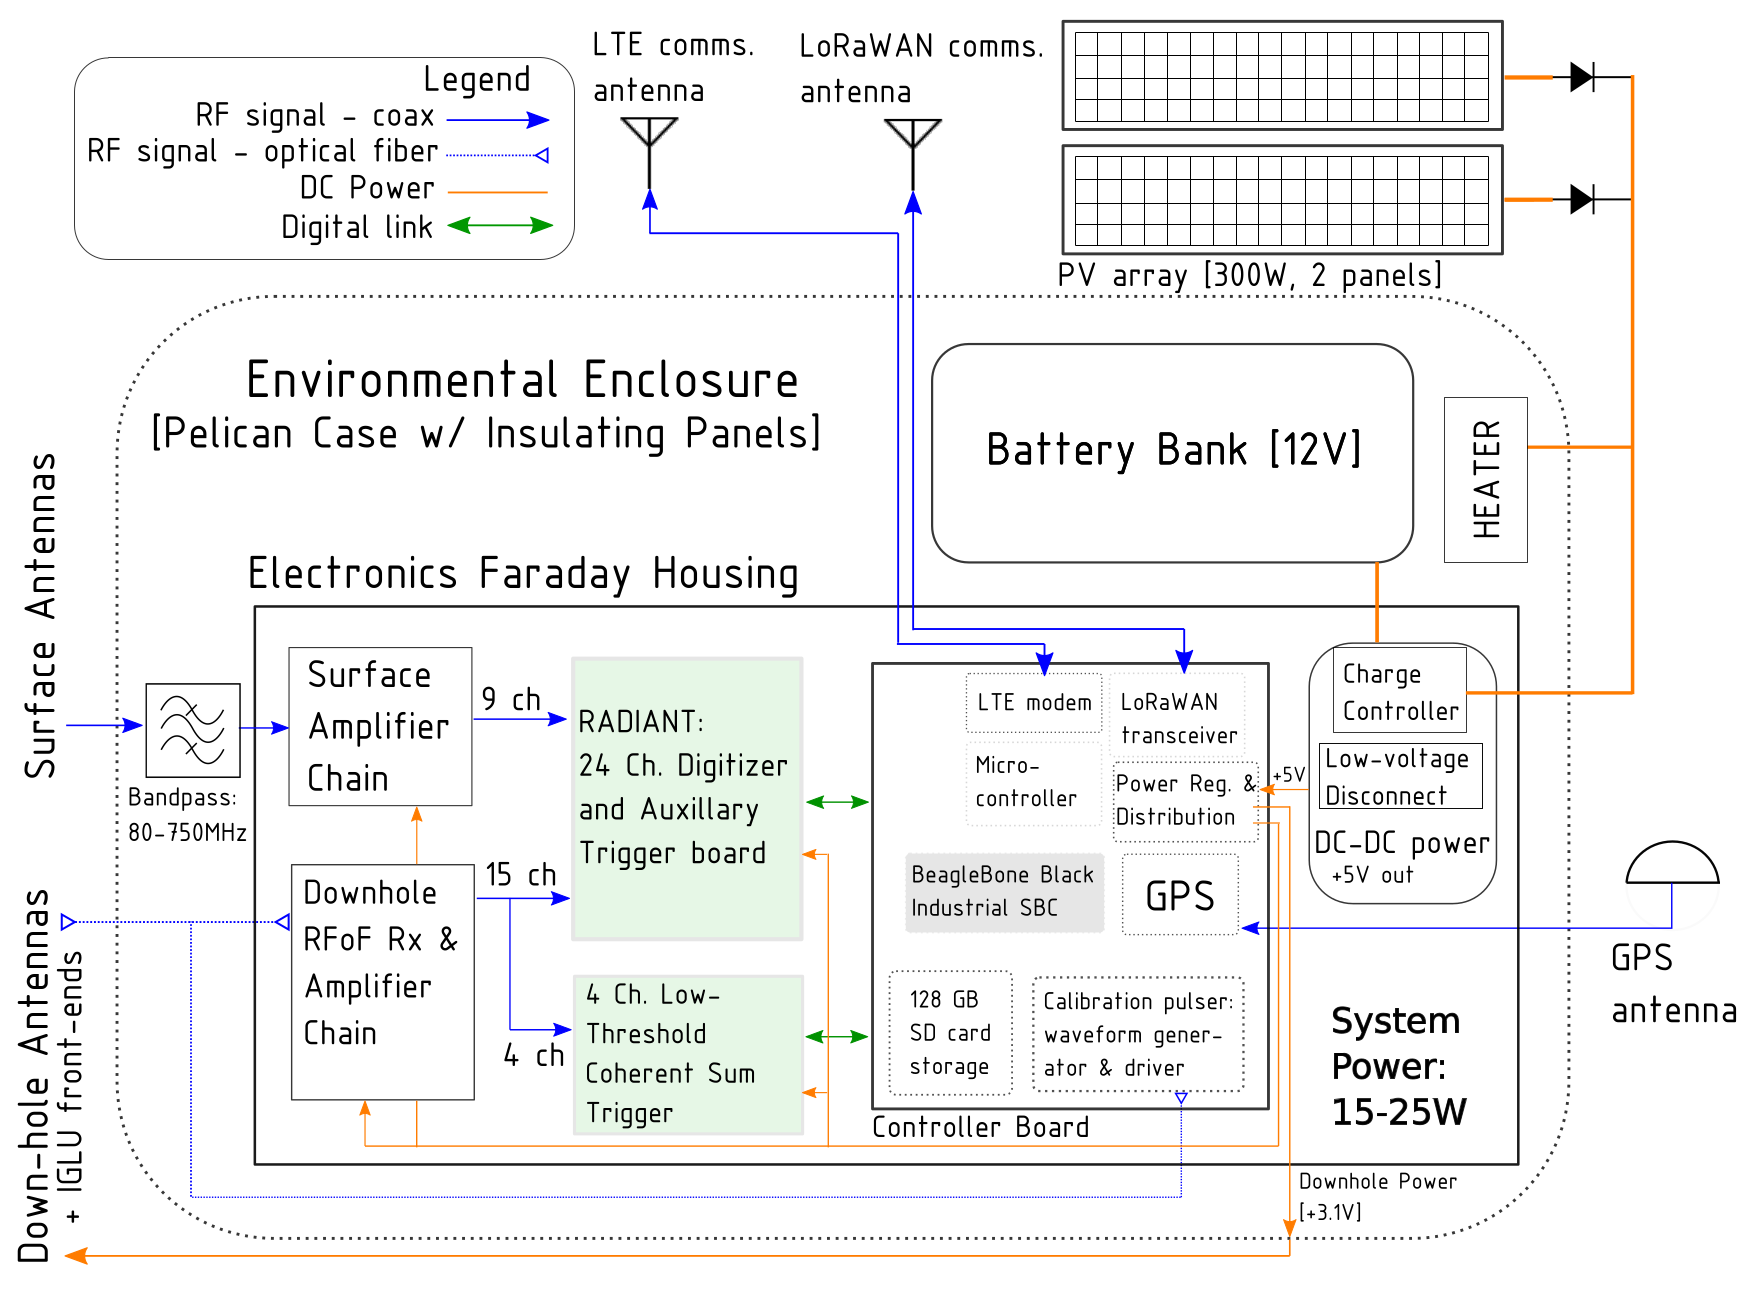
\includegraphics[width=0.9\textwidth]{SysDiagRNOG.png}}{\textcopyright Design and Sensitivity of the Radio Neutrino Observatory in Greenland (RNO-G) by J.A. Aguilar et. al}
  \caption{System diagram for a RNO-G station}
  \label{fig:SysDiag}
\end{figure}

A full system diagram for a RNO-G station is shown in figure \ref{fig:SysDiag}, I'll
give a walktrough of how data gets collected.
The signal from each of the deep antennae are fed into a low-noise amplifier
directly above it, from there the signal is send to the data acquisition (DAQ)
system at the surface via a Radio Frequency over Fiber (RFoF) cable.  The
signals coming from the surface antennae are first passed through a Bandpass
filter of 80-750MHz\footnote{i.e a filter that only lets frequencies in this
range pass} prior to both them and the deep component signal ending up in the
RAdio DIgitizer and Auxiliary Neutrino Trigger (RADIANT), there it's again
amplified, digitized and saved onto an SD card. This data is then transmitted
via a Long Term Evolution (LTE) telecommunications network to a local
server\footnote{There is additionally a Long Range Wide Area Network (LoRaWAN)
antenna as backup in case of problems with the LTE network}, from where it is
sent via a sattelite link.

As a power source, battery banks are used whom are charged via solar panels.
But as there is't enough light during the Greenland winters, there're plans to
build wind turbines (with one of the problems being the possibly detectable RF
noise the 'engine' would produce).

As was previously explained the radio signal from a neutrino often travels
along both direct and refracted paths, designated DnR, to the deep array (as shown
on figure \ref{fig:DnR}).
\begin{figure}
  \centering
  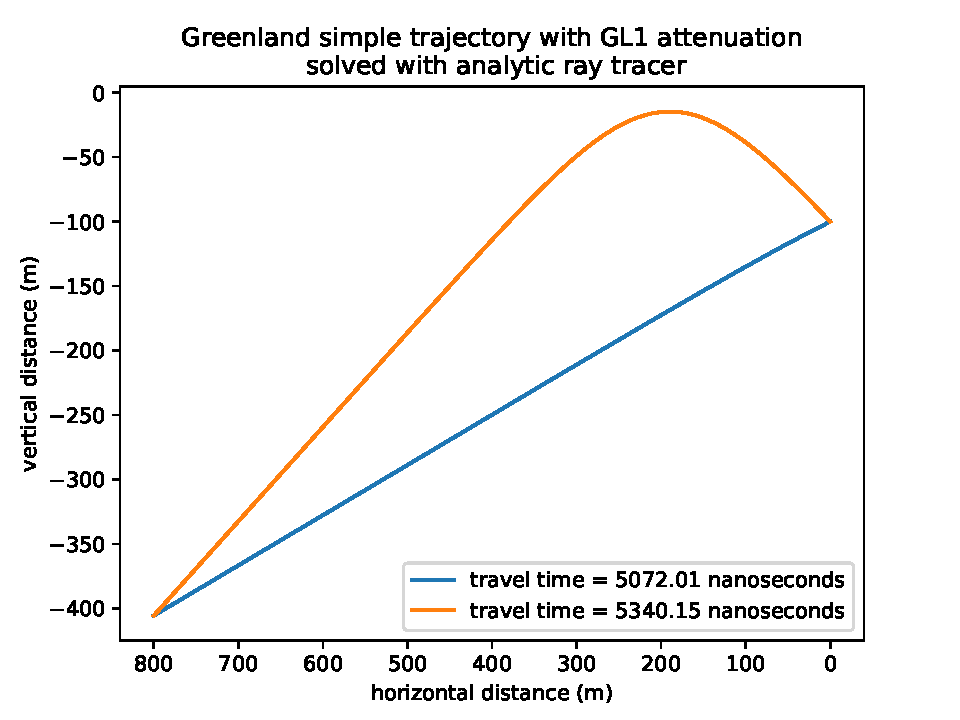
\includegraphics[width=0.5\textwidth]{DnR.pdf}
  \caption{example simulation showing both direct and refracted path from a neutrino vertex (bottom left) to a detector (top right)}
  \label{fig:DnR}
\end{figure}
This double pulse characteristic would be a smoking-gun signature of an in-ice
source. The two helper strings are needed for a full direction reconstruction.
Three independent measurements are needed for azimuthal information, which is
provided by the Vpol (Vertical polarization) antennas and placing the Hpol
(Horizontal polarization) antennas at different depths on every string, both
zentih and azimuth information will be provided for those signals. The helper
strings' calibration pulsers, as well as one on the surface, will ensure
regular monitoring of the performance of the station and provide information
useful for precise calibration of the antenna geometry.
\subsection{Reconstruction: Lookup tables}
The main simulation code we'll be using consists of 2 parts:
NuRadioMC\cite{Glaser_2020} and NuRadioReco\cite{Glaser_2019}. NuRadioMC uses
Monte Carlo simulations to generate neutrino events in the ice and simulates
how they propagate to the various channels, which will be covered more in-depth
in the next chapter. NuRadioReco is reconstruction software, it simulates how
the various detectors would respond to the detected radiowaves. This simulation
software is needed as the plan is to simulate a lot of neutrino events and
record the detector responses in a giant database, then, when an actual neutrino
event occurs, we'll only have to look in the database and match the actual
detector response to the simulated detector responses, thus finding the origin.
\begin{figure}
	\centering
	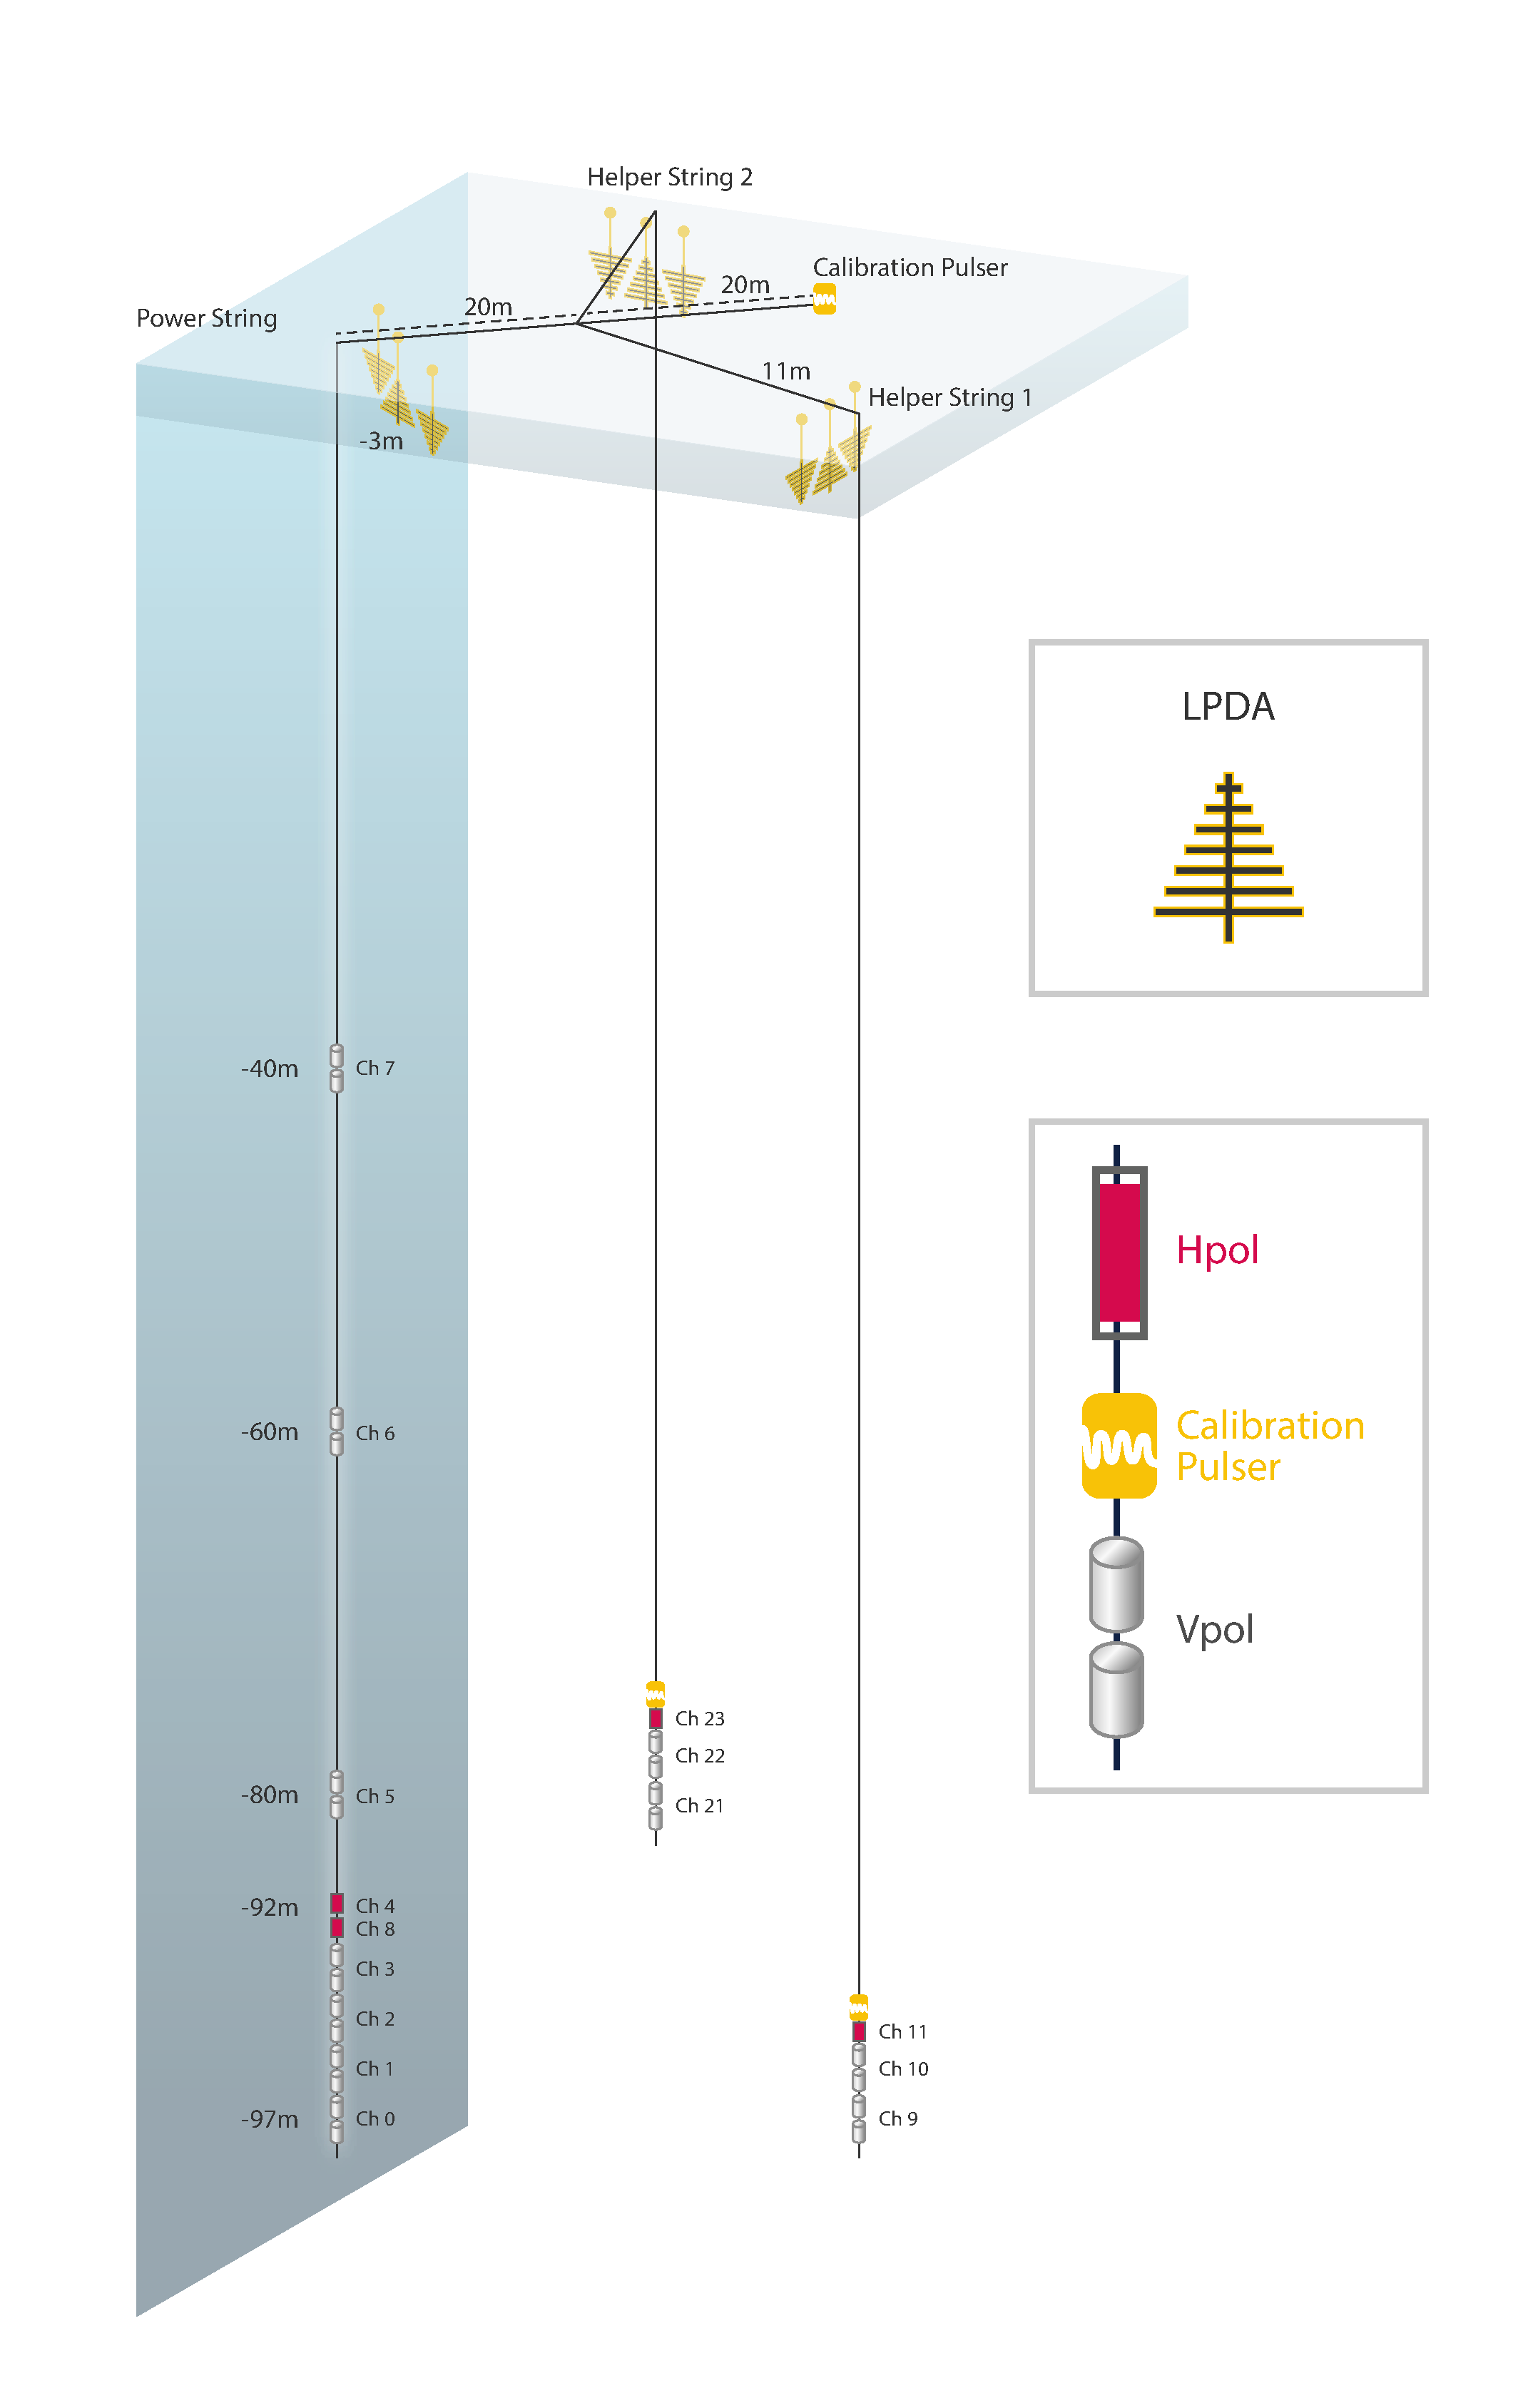
\includegraphics[height=0.9\textheight]{figures/detector.pdf}	
	\caption{diagram showing the numbering and locations of the various antennae}
	\label{fig:detector}
\end{figure}
\begin{figure}
	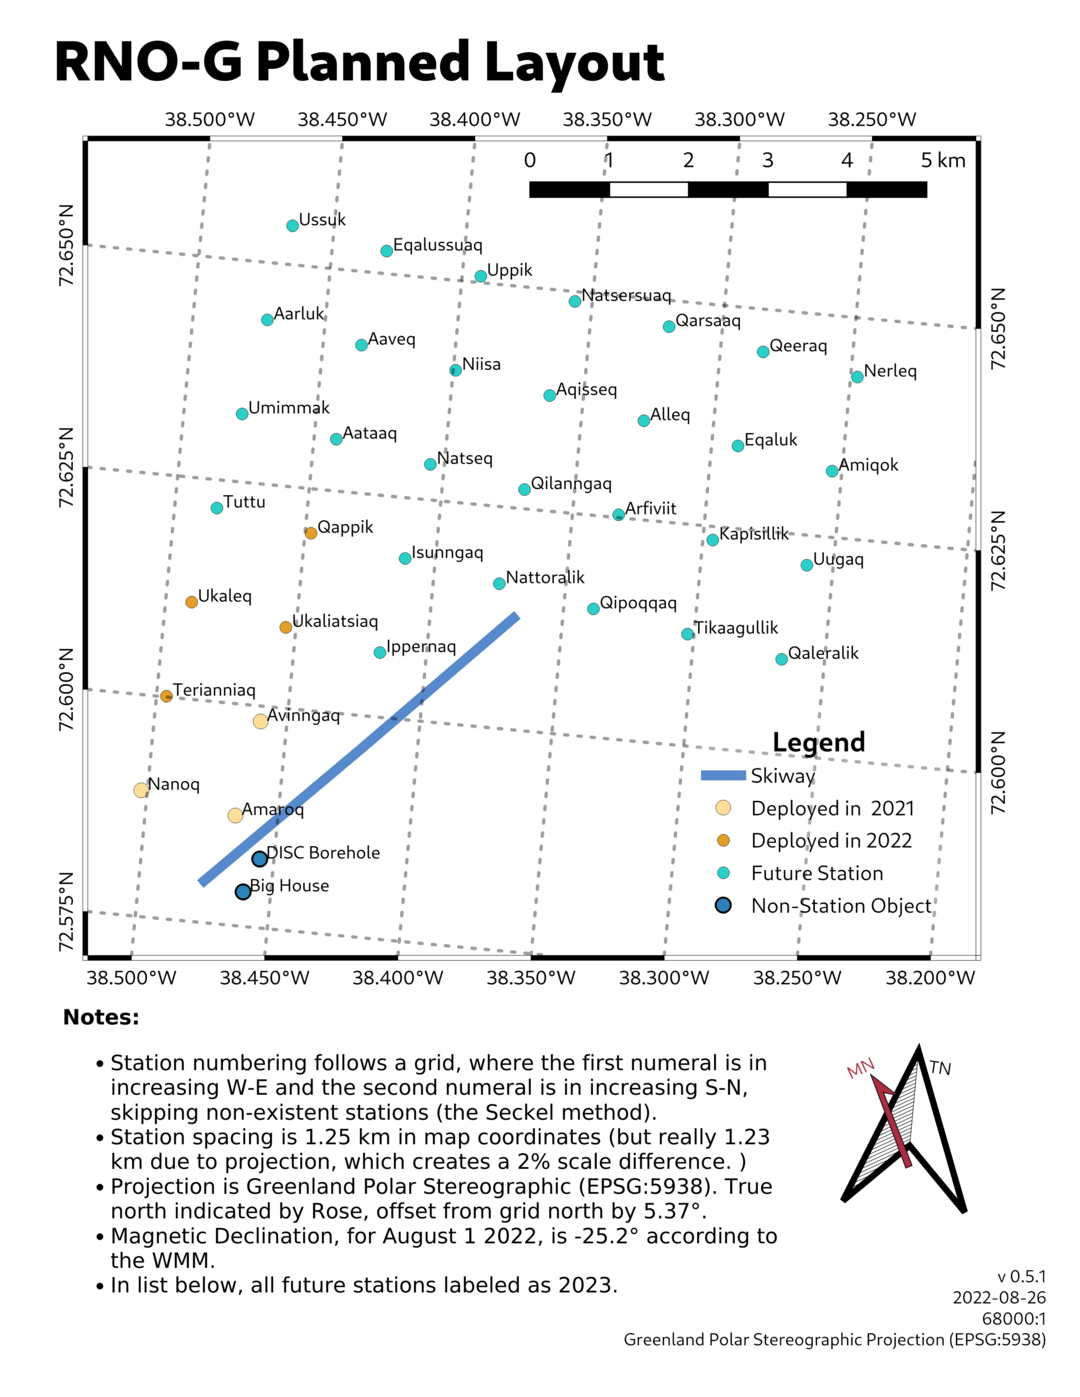
\includegraphics[width=\textwidth]{figures/station-map.png}	
	\caption{planned station layout}
	\label{fig:station map}
\end{figure}

\chapter{Ray tracing}
As previously hinted it is necessary to be able to simulate how radio waves
propagate through the ice to build up a database or just simulate how actual
events would look like.

It will also become necessary in the last chapter for doing actual measurements,
that's why in this chapter we'll give a brief introduction to the way radiowave
paths are found within the NuRadioMC framework.
\section{Wave propagation}
\begin{figure}[h!]
	\centering
	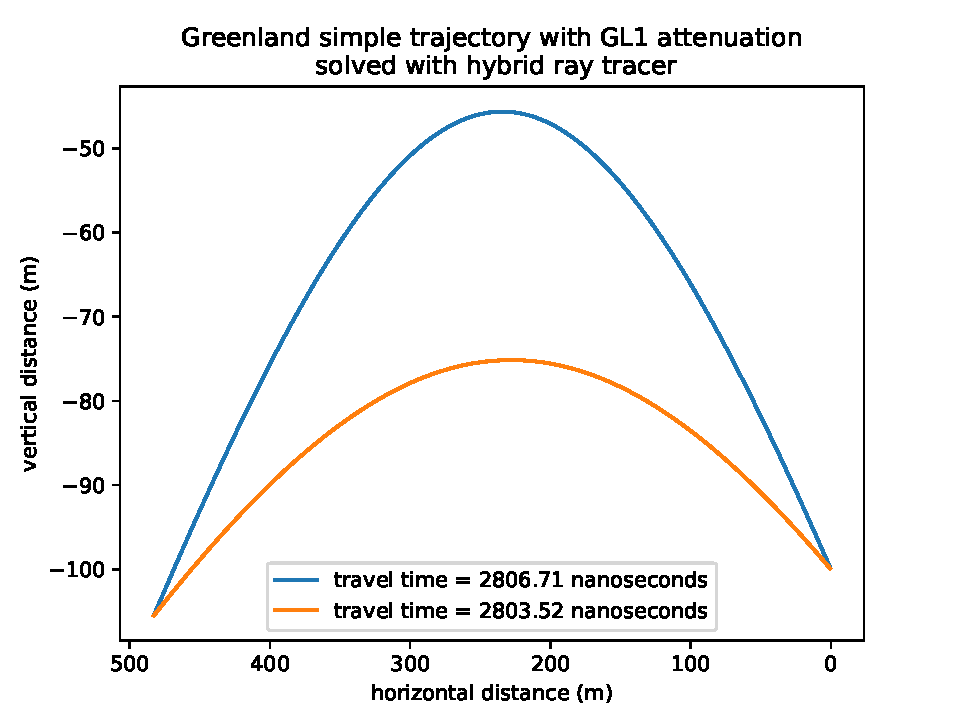
\includegraphics[width=0.7\textwidth]{path_illustration.pdf}
	\label{fig:PathIllu}
	\caption{illustration of radiowave paths generated by a neutrino event}
\end{figure}
The way we simulate the strongest waves propagating to the detector from a
radio source is through ray tracing, an illustration of such a simulation is
shown in figure \ref{fig:PathIllu}.  Here the detector is located at (0,-100)
and a radio source at (480,-108), note that there are two possible paths
leading to the detector.

The amount of solutions and how the waves are bent are consequences of the
properties of the ice we work in.  In a dielectric medium a ray propagates with
it's signal wave-speed determined by the local index of refraction as $v =
c/n$.   The effect on speed isn't the only effect the index of refraction has
which we'll need to concern ourselves with however, if a ray propagates towards
a boundary dividing 2 media with different indexes of refraction, the ray will
refract and the refracted angle can be found from Snell's law:
\begin{equation}
	n_i\sin{\theta_i} = n_o\sin{\theta_o}
\end{equation}
Where n is the index of refraction, $\theta$ the angle with respect to the
surface normal and "i" and "o" indicating incoming and outgoing respectively.
The system we'll consider however, isn't homogeneous with some specified
boundary, it's continous: ice in greenland has a continously varying density and
index of refraction.

How do we know how the waves propagate in a medium?  The software we'll be
using to simulate how the radio waves behave is called \textit{Radiopropa}
\cite{Winchen_2019}. As  simulations of the wave propagation in full detail
with the finite-differences-time-domain (FDTD) technique \cite{1138693} are,
even though they are more accurate, too time consuming. Have the authors of
radiopropa opted to build their program on geometrical optics, i.e ray
tracing. A path of a ray $\mathbf{r}(s)$ with path parameter s in a medium
with index of refraction n($\mathbf{r}$) is described by the eikonal
equation\cite{herman2019treatise}:
\begin{equation}
	\frac{d}{ds}\left(n(\mathbf{r})\frac{d\mathbf{r}}{ds}\right) = \mathbf{\nabla} n
\end{equation}
in radiopropa the local paraxial approximation (small angle approximation) is
used, i.e if we assume that in any individual step of the algorithm the change
of the refractive index along the path ds is small it's possible to re-write
the equation as:
\begin{equation}
	n(\mathbf{r})\frac{d^2\mathbf{r}}{ds^2} \approx \mathbf{\nabla} n
	\label{eqn:radiopropaformula}
\end{equation}
Which is then iteratively solved using the Cash–Karp method.  The way you would
go about using this program is thus find a start and end point (e.g a supposed
neutrino interaction point and a detector respectively), "shoot" your ray in a
certain direction for which the path will then be iteratively solved using
radiopropa and if you chose your direction right you have the path a ray might
take from your start to the end point.  The difficulty is this direction
choosing which we'll get to later.  If there are boundaries (such as defects or
the surface) these are treated seperately using Snell's law. 
\section{Ice model}
\label{section:Ice Model}
Ice has a density gradient which we'll need to account for. Due to the way the
ice bonds there will be more air trapped inbetween the molecules closer to the
surface than at greater depths where the pressure due to the overhead ice
prevents this.  Due to this air being trapped the density of ice will be
smaller closer to the surface than at greater depth.  

Purely from classical gravity and density considerations it can be derived that
the density scales exponentially. To see this let's consider a sheet of ice in
the Greenland firn with a surface A and a height dz, the extra pressure this
sheet of ice exerts on the ice just below it is:
\begin{equation}
	d\sigma = \frac{dF}{A} = -\frac{gdM}{A} = -g\frac{A\rho(z)dz}{A} = -g\rho(z)dz
\end{equation}
with $\rho(z)$ the depth-dependent density. Schytt assumed the
proportional change in air space to be proportional to the change in
pressure:
\begin{equation}
	\frac{dV}{V} \propto d\sigma
\end{equation}
As the volume scales inversely with the density let's assume the relation $V \propto (\rho_i - \rho)$ with
$\rho_i$ the density of pure ice, this yields\cite{herron_langway_1980}:
\begin{align}
	\frac{d\rho}{\rho_i - \rho} &\propto \rho dz\\
	\frac{d\rho}{\rho(\rho_i - \rho)} &\propto \rho dz \label{eqn:SchyttEnd}\\
	\frac{\ln\left(\frac{\rho}{\rho_i-\rho}\right)}{\rho_i} + C &= Az\\
	\ln\left(\frac{\rho}{\rho_i-\rho}\right) &= A\rho_iz + C\\
	\frac{\rho}{\rho_i-\rho} &= e^{A\rho_iz + C} := Ae^{z/z_0}\\
	\rho &= \frac{A\rho_i e^{z/z_0}}{1 + Ae^{z/z_0}}
\end{align}
Note that Schytt worked with equation \ref{eqn:SchyttEnd} but we found
the further derivation useful. Schytt also empirically fitted the
following function:
\begin{equation}
	\label{eqn:myderiexp}
	\rho = \rho_0 e^{z/z_0} + B
\end{equation}
Figure \ref{fig:DensityMeasurements} shows how both of these
functions fit the density curve.  There is one big downside however,
it seems that the ice actually doesn't follow these exponential
curves perfectly but would more closely follow some kind of higher
order function.
\begin{figure}
  \centering
	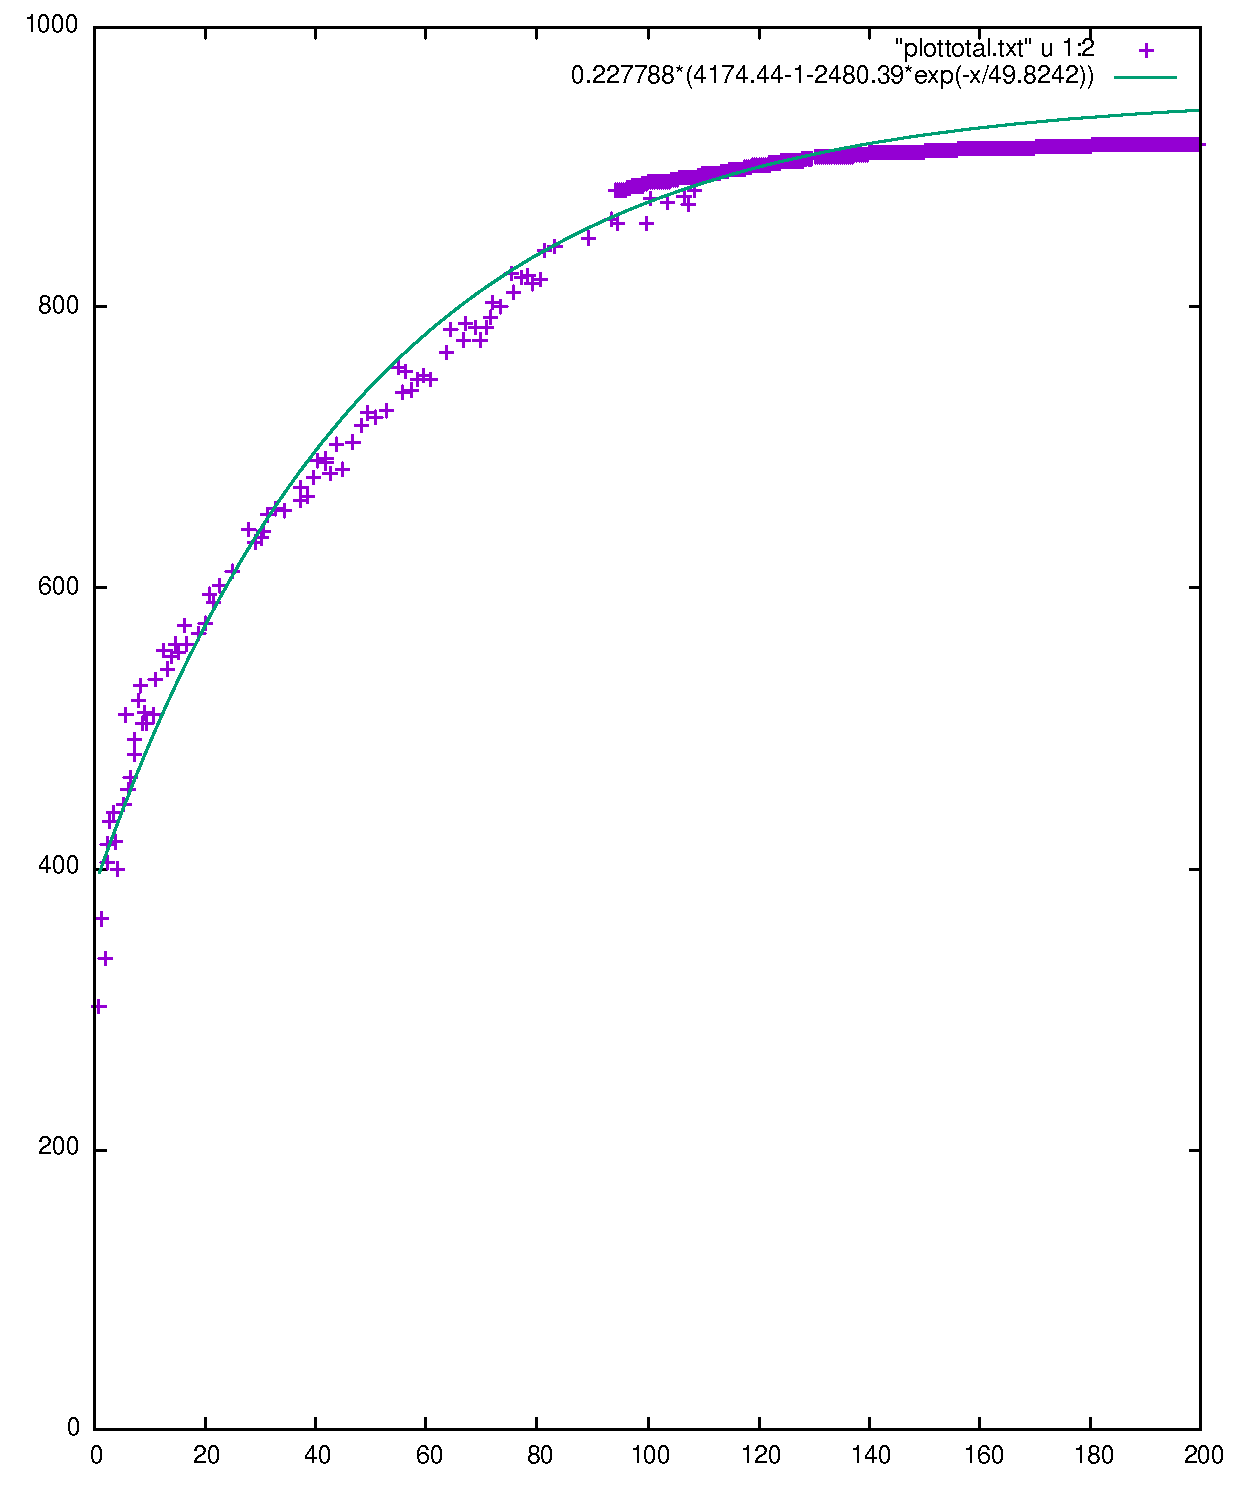
\includegraphics[width=0.5\textwidth]{Density_measurements2.pdf}
	\caption{Illustration of the shortcomings of the analytical models}
	\label{fig:DensityMeasurements}
\end{figure}

Equation \ref{eqn:radiopropaformula}, and thus the path, depends on the index
of refraction on a given location.  The dependence of the index of refraction
on density for ice can approximately be given by the Schytt equation\cite{Barwick_2018}:
\begin{equation} 
	n(x,y,z) \approx 1 + 0.78\rho(x,y,z)/\rho_0 \label{eqn:Schytt}
\end{equation} 
Where $\rho(x,y,z)$ is the local ice density and $\rho_0$ is the
density for solid ice (917 kg/m³).  For the development of the simulation
software equation \ref{eqn:myderiexp} was taken and after assuming Schytt's
equation to hold we find that the index of refraction abides by
\begin{equation}
	\label{eqn:expn}
	n(z) = n_{ice} - \Delta n e^{z/z_0}
\end{equation}
with $n_{ice}$ the refractive index of solid ice and $\Delta n = n_{ice} - n_s$
with $n_s$ the index of refraction of snow. This exponential dependency of the
index of refraction on depth is called the \textit{single exponential model}.  

This single exponential model has a huge advantage as it's analytically
solvable, meaning that we can know which direction we'll have to shoot our ray
in (as mentioned previously) after the location of the neutrino interaction and
the detector are specified, the ray tracing algorithm developed using this
exponential index is called the \textit{analytic ray tracer}.

The discrepency between the single exponential model and the actual data for
the density implies that the analytic ray tracer will make the wrong
predictions.  This is why the development of a different ray tracer was needed
which will be able to handle more complex ice models, one such ray tracer will
be explained in section \ref{sec:Iterative} but this ray tracer has it's
shortcomings. That's why the development of a new ray tracer was needed which
is the partial work of this thesis and we'll get to that ray tracer in chapter
\ref{chapter:hybrid}.

\begin{figure}
  \centering
  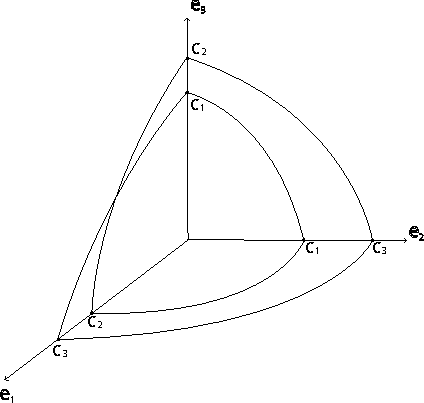
\includegraphics[width=0.5\textwidth]{figures/Fresnel.pdf}
  \caption{Wave surface of Fresnel with two sheets}
  \label{fig:Fresnel}
\end{figure}
Lastly there is an effect which might become important in the future:
birefringence.  Up until now have implicitly assumed that ice is isotropic
meaning that both it's permittivity $\varepsilon$ and it's permeability $\mu$
are scalars but these could very well be tensorial in nature for radio waves in
ice. In general, after calculating this tensorial nature through you'd find
that in every direction two different indices of refraction can be found
implying two different types of waves each propagating with a different speed
as illustrated in figure \ref{fig:Fresnel}. Which of the two speeds in a
certain direction is then dependent on the polarization of the wave, which in
our case thus depends on the Askaryan effect (see section \ref{sec:Askaryan}).
The optical property coming from the anisotropic nature of the material is
what's called \textit{birefringence}.  Birefringence has been extensively
researched for implementation in the simulation software NuRadioMC used in the
RNO-G group \cite{Heyer2023}.
\section{Iterative ray tracer}
\label{sec:Iterative}
The iterative ray tracer \cite{2022icrc.confE1027O}, as can be derived from
it's name, iteratively searches the path a ray might take. The workings of the
first part of the explanation is illustrated in figure \ref{fig:Illustration of
iterative algorithm}.  
\begin{figure}
  \centering
  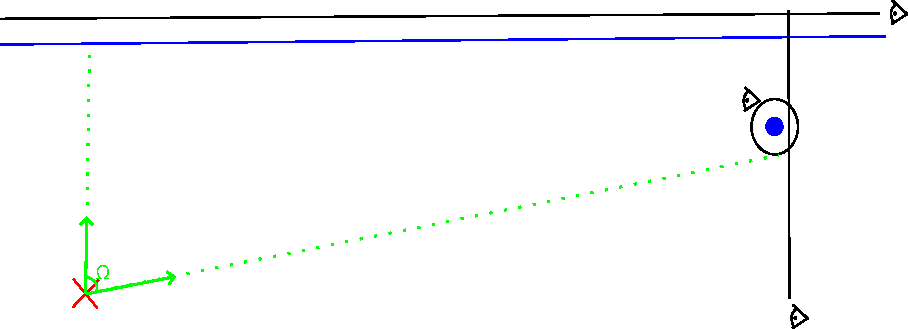
\includegraphics[width=0.7\textwidth]{algoillu.pdf}
  \caption{Illustration of the workings of the iterative algorithm}
  \label{fig:Illustration of iterative algorithm}
\end{figure}
Say we have a neutrino interaction point $\mathbf{X}_i$
(the red cross on the figure) and a detector located at $\mathbf{X}_d$ (the
blue dot on the figure), the algorithm starts by constructing an
\textit{observer} sphere with radius $r_1$ with the detector, located at $\mathbf{X}_d$, as the
center.  This means that any ray that gets shot and propagates to the sphere
will get stopped and counts as a solution.  Then, to reduce the time spent simulating, there are also observers placed
whose purpuse is to stop the ray tracing but not count the observed signal as a solution.
One such observer is placed 
just above the ice surface as a ray that escapes the ice won't be able to make it back, and one
is placed just behind the detector looking from the point of the interaction vertex $\mathbf{X}_i$ as
a ray is not able to reach the detector anymore after it has passed it in the
lateral direction. Finally it's noted that due to the way the ice's index of refraction
continuously increases with depth, rays can't propagate upwards, this means that we only 
have to look for solutions within the angle $\Omega$ which is just the zenith angle the detector
makes with the bottom of the observer sphere.
Now that we have our setup we'll just iteratively shoot rays from the neutrino
interaction point starting at an angle $\Delta \theta_1$ then at an angle
$2\Delta \theta_1$, $3\Delta \theta_1$,... Until we have reached $\Omega$. This
process is illustrated on the left side of figure \ref{fig:IterativeWorkings}.
\begin{figure}
  \centering
  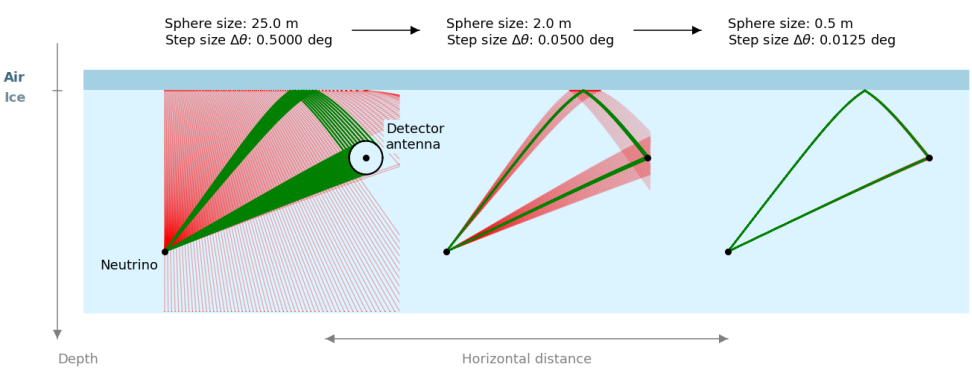
\includegraphics[width=0.7\textwidth]{IterativeWorkings.png}
  \caption{Illustration of the steps of the iterative ray tracer}
  \label{fig:IterativeWorkings}
\end{figure}
After we have gone over all the different launch angles we'll have some
solutions (marked in green) and some whom don't end up on the detector (marked
in red) we can now make the observer sphere's radius smaller ($r_2 < r_1$) and
the step size of the angle smaller ($\Delta \theta_2 < \Delta \theta_1$).  And
again iteratively find the rays which end up on the sphere, only this time
looking within the angles of the solutions of the previous step. We can keep on
making the sphere and step size smaller in iterative steps until we've reached
the precision we want. We then take, for each bunch of solutions within an
angle interval, the most normal to the detector as the final solutions.


\chapter{Hybrid Ray tracer}
\label{chapter:hybrid}
%----------------------------------------------------------------------------------------
%	HYBRID RAY TRACER	
%----------------------------------------------------------------------------------------
\section{Shortcomings of the exponential ice model}
As mentioned in section \ref{section:Ice Model}, complex ice models will be
necessary moving forward as the exponential ice model fails to fit the density
curve.  The software for radio wave propagation through ice the RNO-G team
chose is radiopropa\cite{Winchen_2019}, but due to the way it works you'll have
to know the start point, the end point and the launch angle of your ray to work
out the path. This isn't difficult for the analytic model as it's exactly
solvable but for a general ice model you'll somehow have to find where to
\textit{shoot} the ray. An algorithm was developed to work out the path the
rays would trace out in more complex ice models called the \textit{iterative
ray tracer} \cite{2022icrc.confE1027O}, which was discussed in section
\ref{sec:Iterative}. The way this algorithm works is however a sub-optimal
solution in python as an optimalisation library will generally work faster and
more accurate, work had been done on trying to implement such an algorithm
deemed the "minimizer" but this attempt failed.  As we saw this work the idea
came to mind to combine the iterative ray tracer and the code using the
optimization libraries. This way we built the algorithm which will be discussed in
this chapter: The hybrid ray tracer, in the source code called the "hybrid
minimizer" which can be found
\href{https://github.com/arthuradriaens-code/NuRadioMC.git}{here} under the
radiopropa/hybrid\_minimizer branch.

It succeeds in more rapidly finding the path from the event to the detector, is
more accurate and also arrives closer to the detector as the final result is
not limited by the final drawn sphere size but by a given tolerence making it
useful for plane wave reconstruction as we'll get to in the next chapter.

\section{How it works}
The hybrid minimizer can be seen as an extension of the iterative raytracer as
it starts out the same way: Say our source of radiation is at position
$\mathbf{X}_1$ and our detector is located at position $\mathbf{X}_2$, we start
by defining the vector $\mathbf{v} = \mathbf{X}_2 - \mathbf{X}_1$, then we
clone it as a new vector $\mathbf{u}$ and set it's z coordinate to 0, making it a normal
vector of a plane parallel to the z direction in the lateral direction of the detector. 
We now want to constrain the search to where solutions are actually possible
, looking at figure \ref{fig:PathIllu}
we see that no solutions below the direct path are possible as there would need
to be upwards reflection, so we convert our vector $\mathbf{v}$ representing
the path from the source to the detector to spherical coordinates, giving us a
polar angle (zenith angle) "theta-direct". With this we know that from the source
the ray should propagate with an initial zenith angle lying within the angle interval
0° to theta-direct° $:= \Omega$ ($\theta \in ]0,\Omega]$).

Next we need to define our "observers", if you shoot a ray with the radiopropa
module from a certain point at a certain angle the ray path will get simulated
until it interacts with this "observer".  Ideally we would like to a priori
know where to shoot our ray and have the detector be an infinitesimally small
observer in our simulation, but as we'll be working with general ice models
this can't be done.

The algorithm of finding the possible paths is then as follows: We define a
spherical observer at the location of the detector, with a radius of fair
size\footnote{We'll get back to this}.  We place an observer plane directly
behind the detector with normal vector $\mathbf{u}$ (as no rays can propagate
back after passing the detector) and an observer above the surface (as no rays
could make it back after escaping the ice) our full setup is then what's
illustrated in figure \ref{fig:Illustration of hybrid algorithm}

\begin{figure}
  \centering
  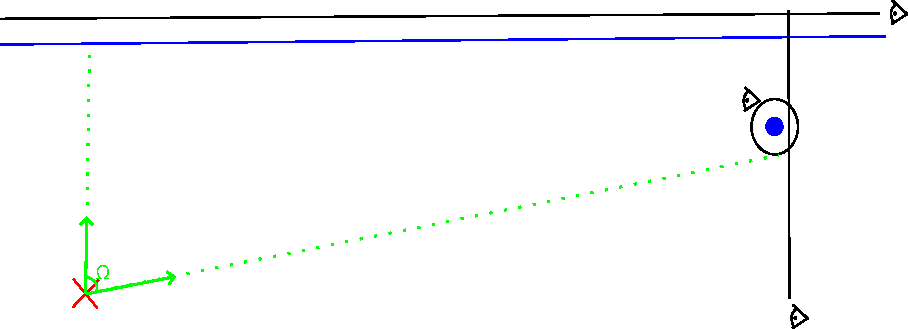
\includegraphics[width=0.7\textwidth]{algoillu.pdf}
  \caption{Illustration of the workings of the hybrid algorithm}
  \label{fig:Illustration of hybrid algorithm}
\end{figure}

Here the red cross is the radio source, the blue horizontal line is the ice-air
boundary surface, the blue dot to the right is the detector and the green
$\Omega$ indicates the range over which solutions to the problem are possible.

We start off by just iteratively guessing: given a certain angle stepsize
$\Delta \theta$ shoot rays at the angles $\{0,\Delta \theta, 2\Delta
\theta,...,\Omega\}$ And see which ones get detected at the sphere around the
detector, this process is illustrated in figure \ref{figure:First step hybrid}.
\begin{figure}
	\centering
	\copyrightbox[r]{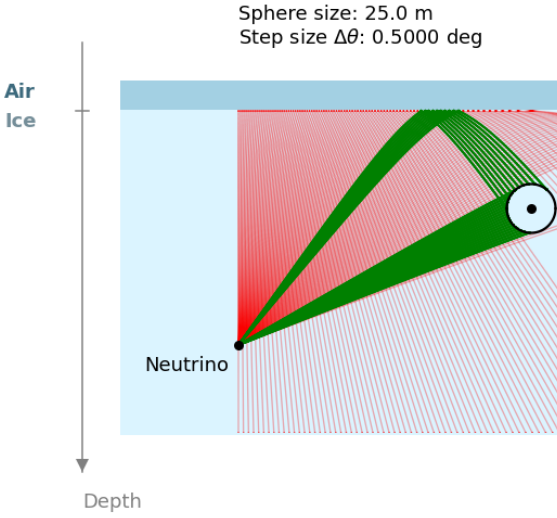
\includegraphics[width=0.5\textwidth]{begin_explanation.png}}{\textcopyright Effects of firn ice models on radio neutrino simulations using a RadioPropa ray tracer by B. Oeyen et. al}
	\caption{First step of the hybrid ray tracer}
	\label{figure:First step hybrid}
\end{figure}
if 2 distinct launch regions are found, the so called \textit{minimization}
procedure will start. Using scipy's module optimize.minimize the optimal
solution will be found. First we get rid of the spherical observer and place
the vertical observer \textbf{exactly} at the detector, now to be able to use the
minimize module we'll need a function to minimze, for this reason we first define the
function \textit{delta\_z} as, given a certain launch angle, propagating the ray
onto the vertical observer and returning the
distance from the point where it lands on the plane to the detector, as
illustrated on figure \ref{fig:PrincipleHybridIllu} (i.e it returns the value $\Delta z$).
\begin{figure}
  \centering
  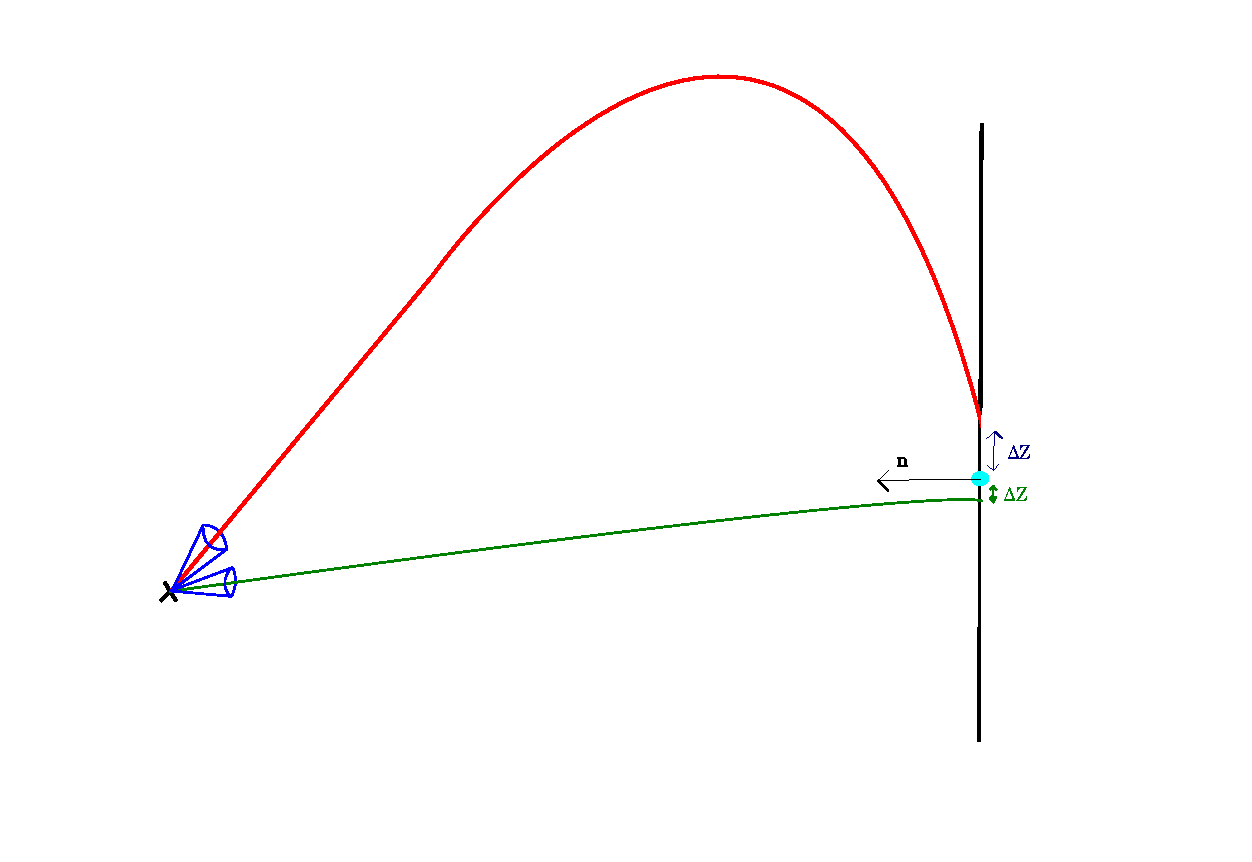
\includegraphics[width=0.5\textwidth]{PrincipleHybridIllu.pdf}
  \caption{Principle behind the minimization in the hybrid ray tracer}
  \label{fig:PrincipleHybridIllu}
\end{figure}
The function we'll minimize is then delta\_z\_squared which just squares the
value which delta\_z returns as we want to do away with negative values (so we
can minimize to $\Delta z=0$). We use the previously found angle boundaries as
the boundaries for this minimization algorithm, meaning that if the 2 zenith
angle intervals $[\theta_1,\theta_2]$ and $[\theta_3,\theta_4]$ were found in
the first step of the algorithm it will first minimize $\Delta z^2$ within the
first angle interval and find it's solution and then within the second angle
interval. With this our algorithm is done, it does have a fail-safe as well for
if the first step, finding the launch regions, doesn't find the 2 launch
regions.  Namely it reverts back to being the iterative ray tracer.

\section{Performance Optimalisation} 
We wish to optimize this algorithm to make
it as fast as possible.  To consistently test the algorithm after every
particular change in a parameter we'll be randomly generating vertex
interaction positions, keeping the detector at the fixed (0,-100) value.  To
this end the numpy random module was used to generate random coördinates, the
considered square (as there is only a z component to the ice model the 3D
problem is cilindrically symmetric and thus essentially only a 2D problem) is
x:0.1km,4km and z:-0.1km,-3km\footnote{This start at 100m depth was to get
around issues concerning events that won't even trigger in a full simulation}.
Every simulated point shown in the following subsections consists of at least
500 random initial positions.  As the speed of the algorithm is computer
dependent the algorithm's speed is always plotted relative to the iterative ray
tracer's speed, simulated with the same coordinates equal computer load.

Now we don't want to just achieve higher speed in our algorithm, we also want
to at least have the same accuracy as the iterative ray tracer, if not even better.
To this end we need to check with an "exact solution". There is only one candidate
that fits this role: \textit{the analytic ray tracer}. The plan is thus to use the
exponential ice model as a testing ground for the hybrid ray tracer and solving each
vertex-detector ray tracing problem with both the iterative, analytic and hybrid ray tracer.
After having solved for the \textbf{propagation time}, meaning the time it takes the ray to
propagate from the source to the detector. And the \textbf{arrival zenith angle}, the zenith angle
the ray makes at the detector, for each of the algorithms we can infer the accuracy of a particular
algorithm by how much it differs from the solution found through the analytic ray tracer.
For example, if the hybrid ray tracer finds a particular solution with a propagation time of 
1001ns, the iterative finds one with 1002ns and the analytic one with 1000ns then the hybrid
ray tracer is more accurate than the iterative ray tracer.
\subsection{Length of the normal vector}
\begin{figure}
	\centering
	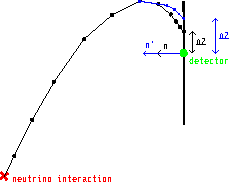
\includegraphics[width=0.7\textwidth]{figures/PrincipleNormIllu.pdf}
	\caption{how normal vector size influences the stepsize}
	\label{fig:normexpl}
\end{figure}
Whilst figuring out what was wrong with the initial \textit{minimizer} we
stumbled on the fact that radiopropa has a little weird quirk.  As visually
explained in figure \ref{fig:normexpl}, the size of the normal vector seems to
influence how big radiopropa's ray tracer's step size is taken close to the
detector.  This thus influences the accuracy and total computational time
taken. The results of varying the length of this normal vector, comparing the
accuracy (in timing and arrival zenith) with the analytic ray tracer and the computational time with the
iterative ray tracer, are shown in figures \ref{fig:norminfl} and
\ref{fig:norminfl2}.  Looking at these figures we can conclude a, what would
normally be rather obvious but is interesting nonetheless, first optimization
conclusion: take the normal vector length to be 1 meter.
We can conclude this as the calculation speed seems to be minimal there (after zooming
in on the graph) and the accurace dropping rapidly after 1 meter.

\begin{figure}
	\centering
	\begin{minipage}{\textwidth}
		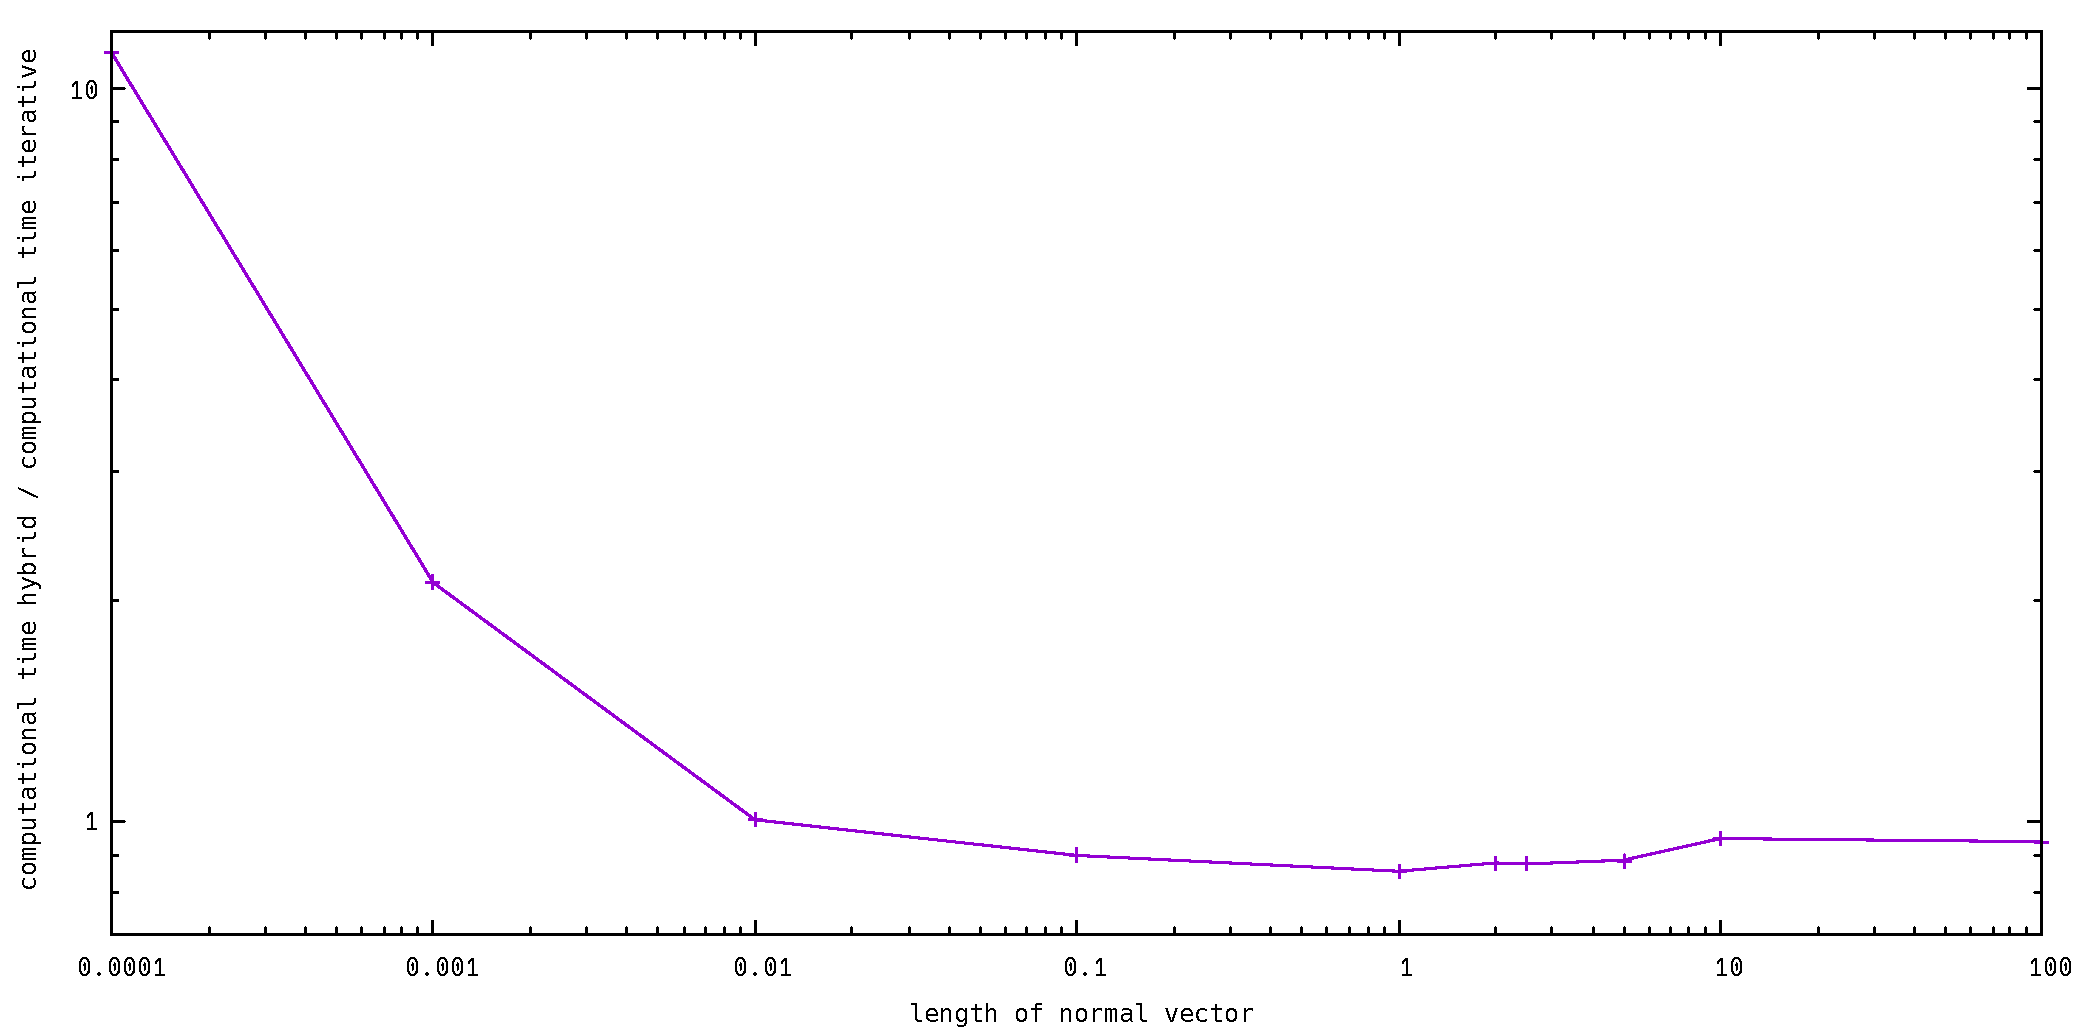
\includegraphics[width=0.8\textwidth]{figures/NormVsTime.pdf}
	\end{minipage}
	\begin{minipage}{\textwidth}
		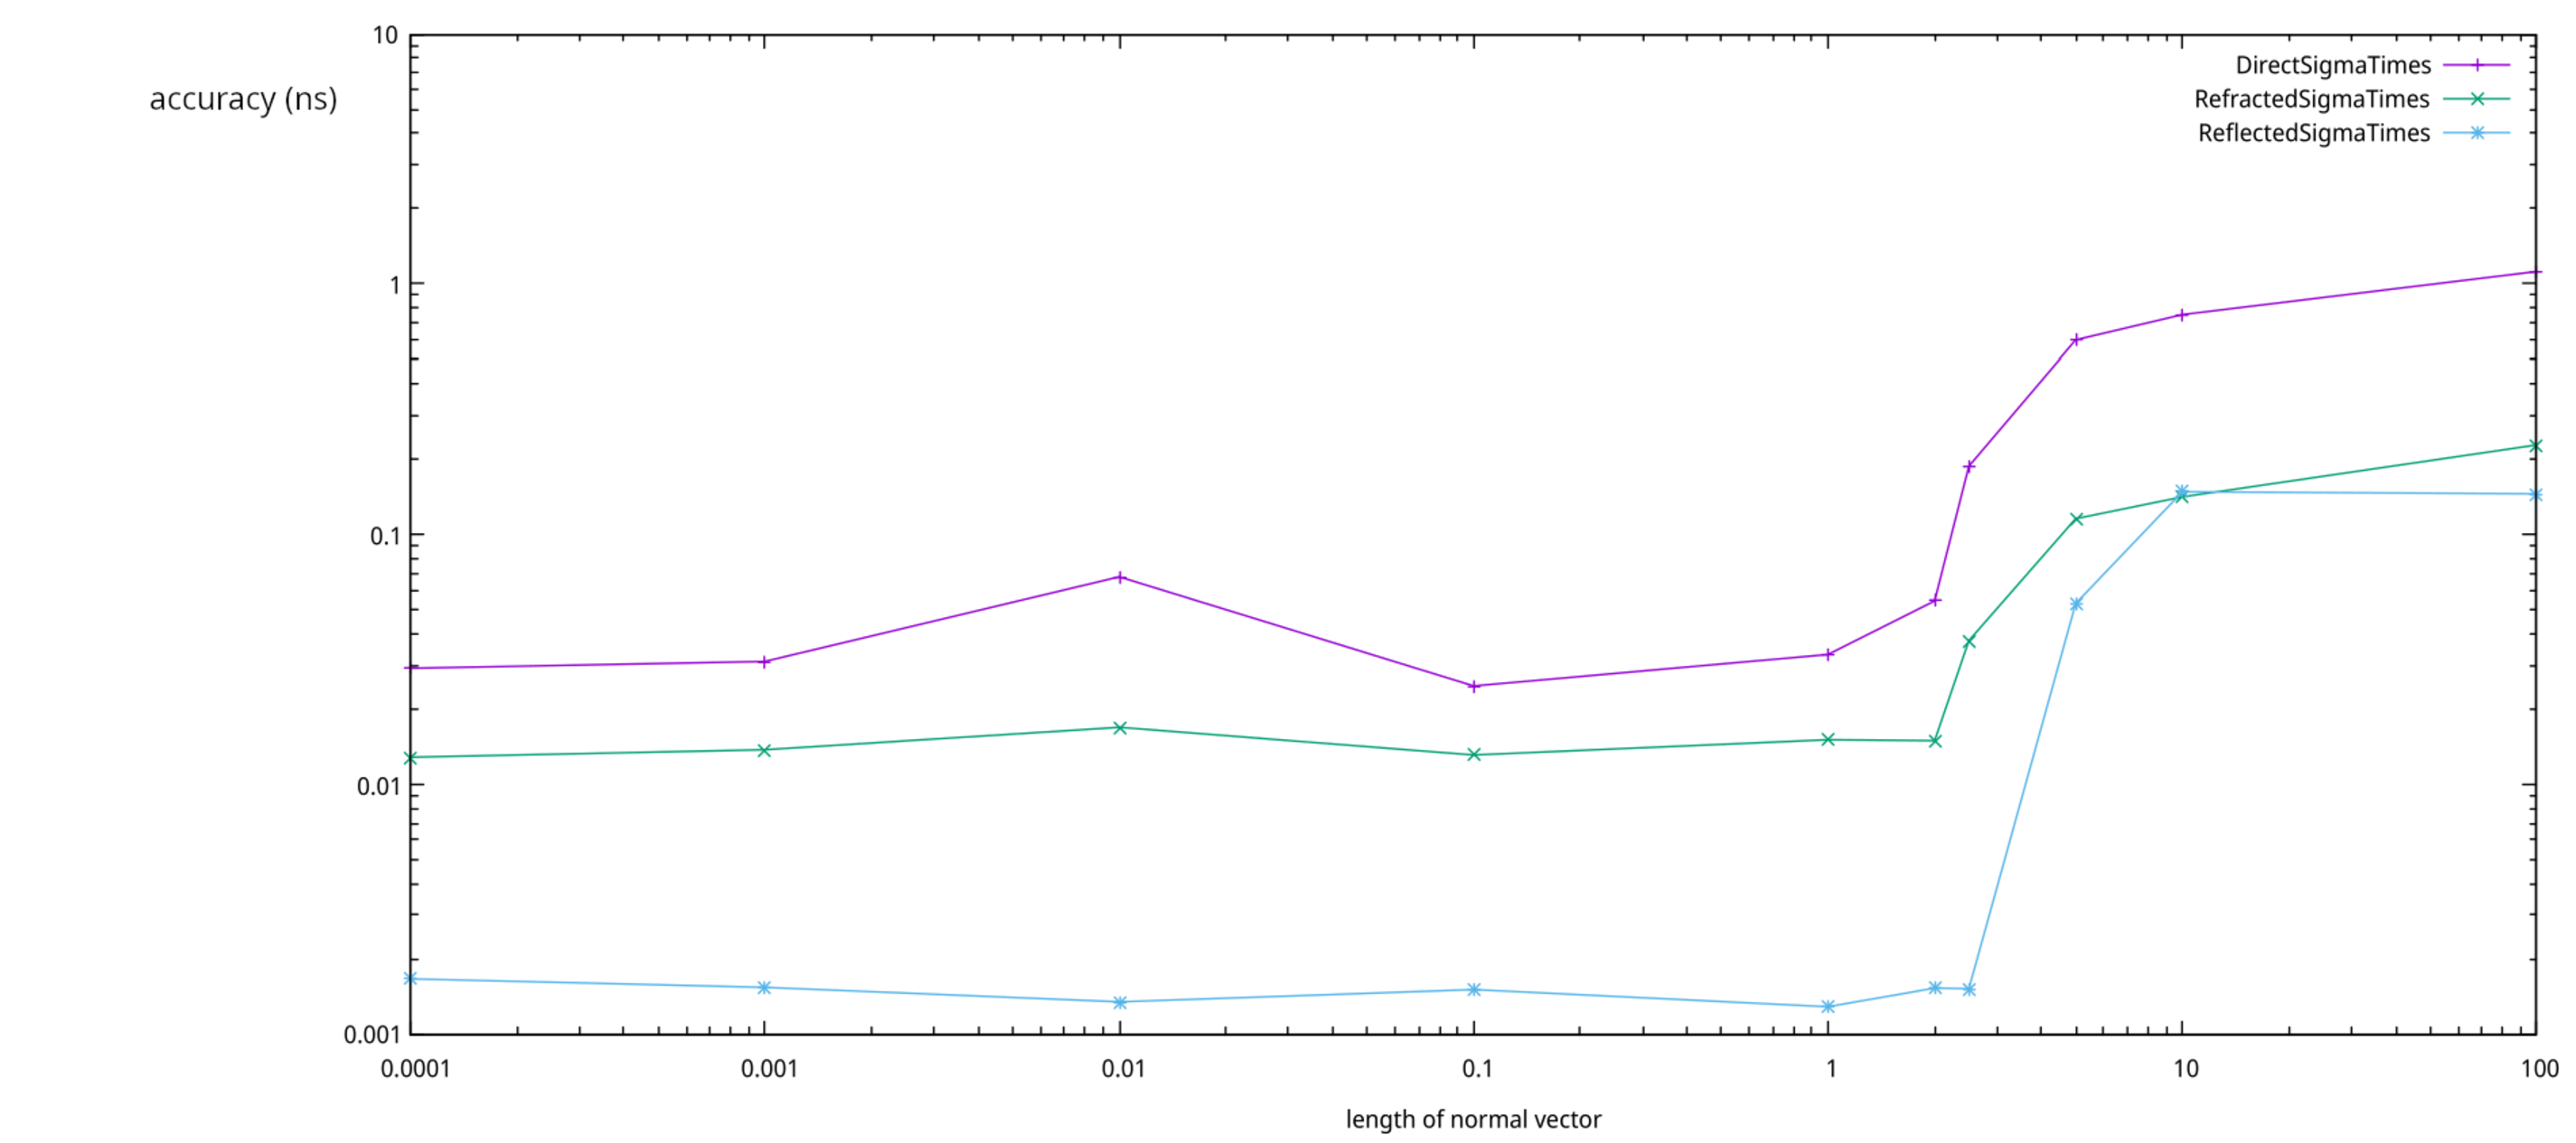
\includegraphics[width=0.8\textwidth]{figures/NormVsSigmaTime.pdf}
	\end{minipage}
\caption{influence of the length of the normal vector}
\label{fig:norminfl}
\end{figure}
\begin{figure}
	\centering
	\begin{minipage}{\textwidth}
		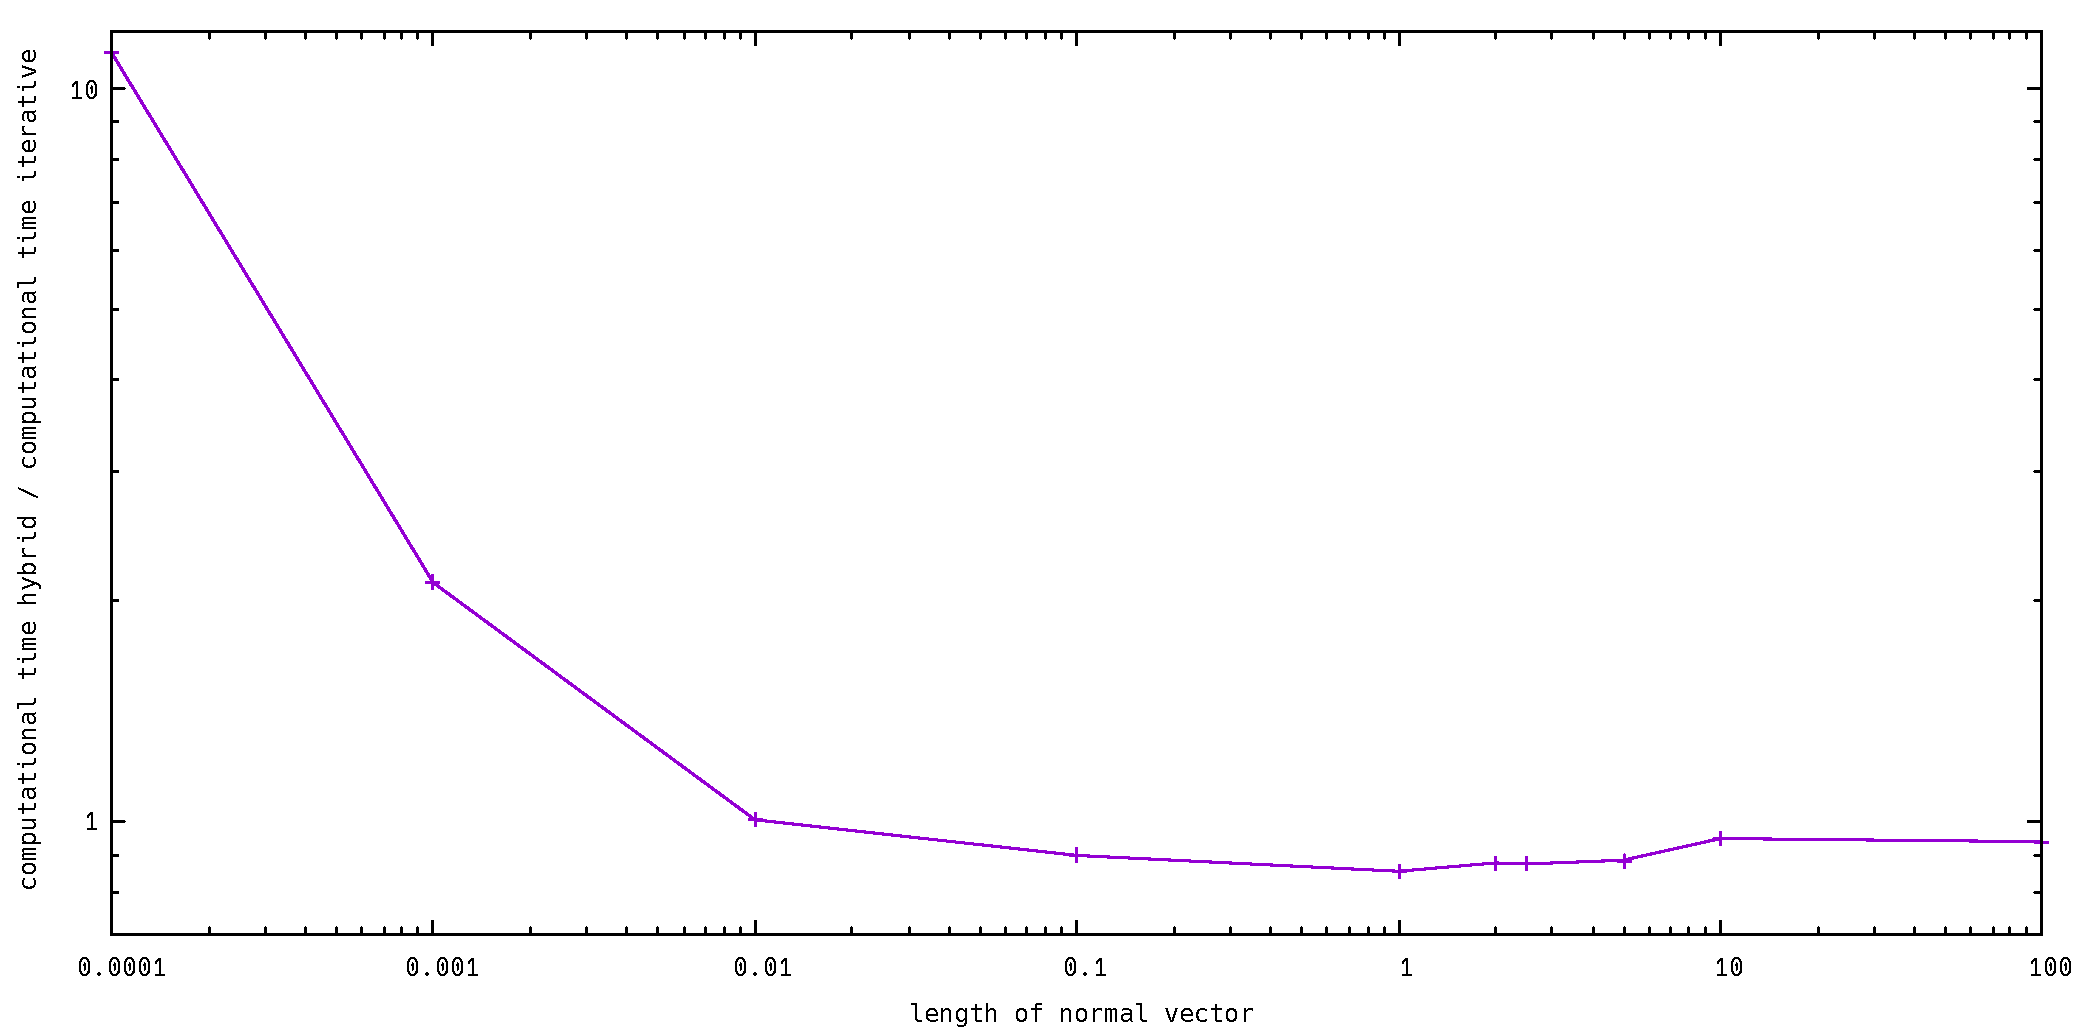
\includegraphics[width=0.8\textwidth]{figures/NormVsTime.pdf}
	\end{minipage}
	\begin{minipage}{\textwidth}
		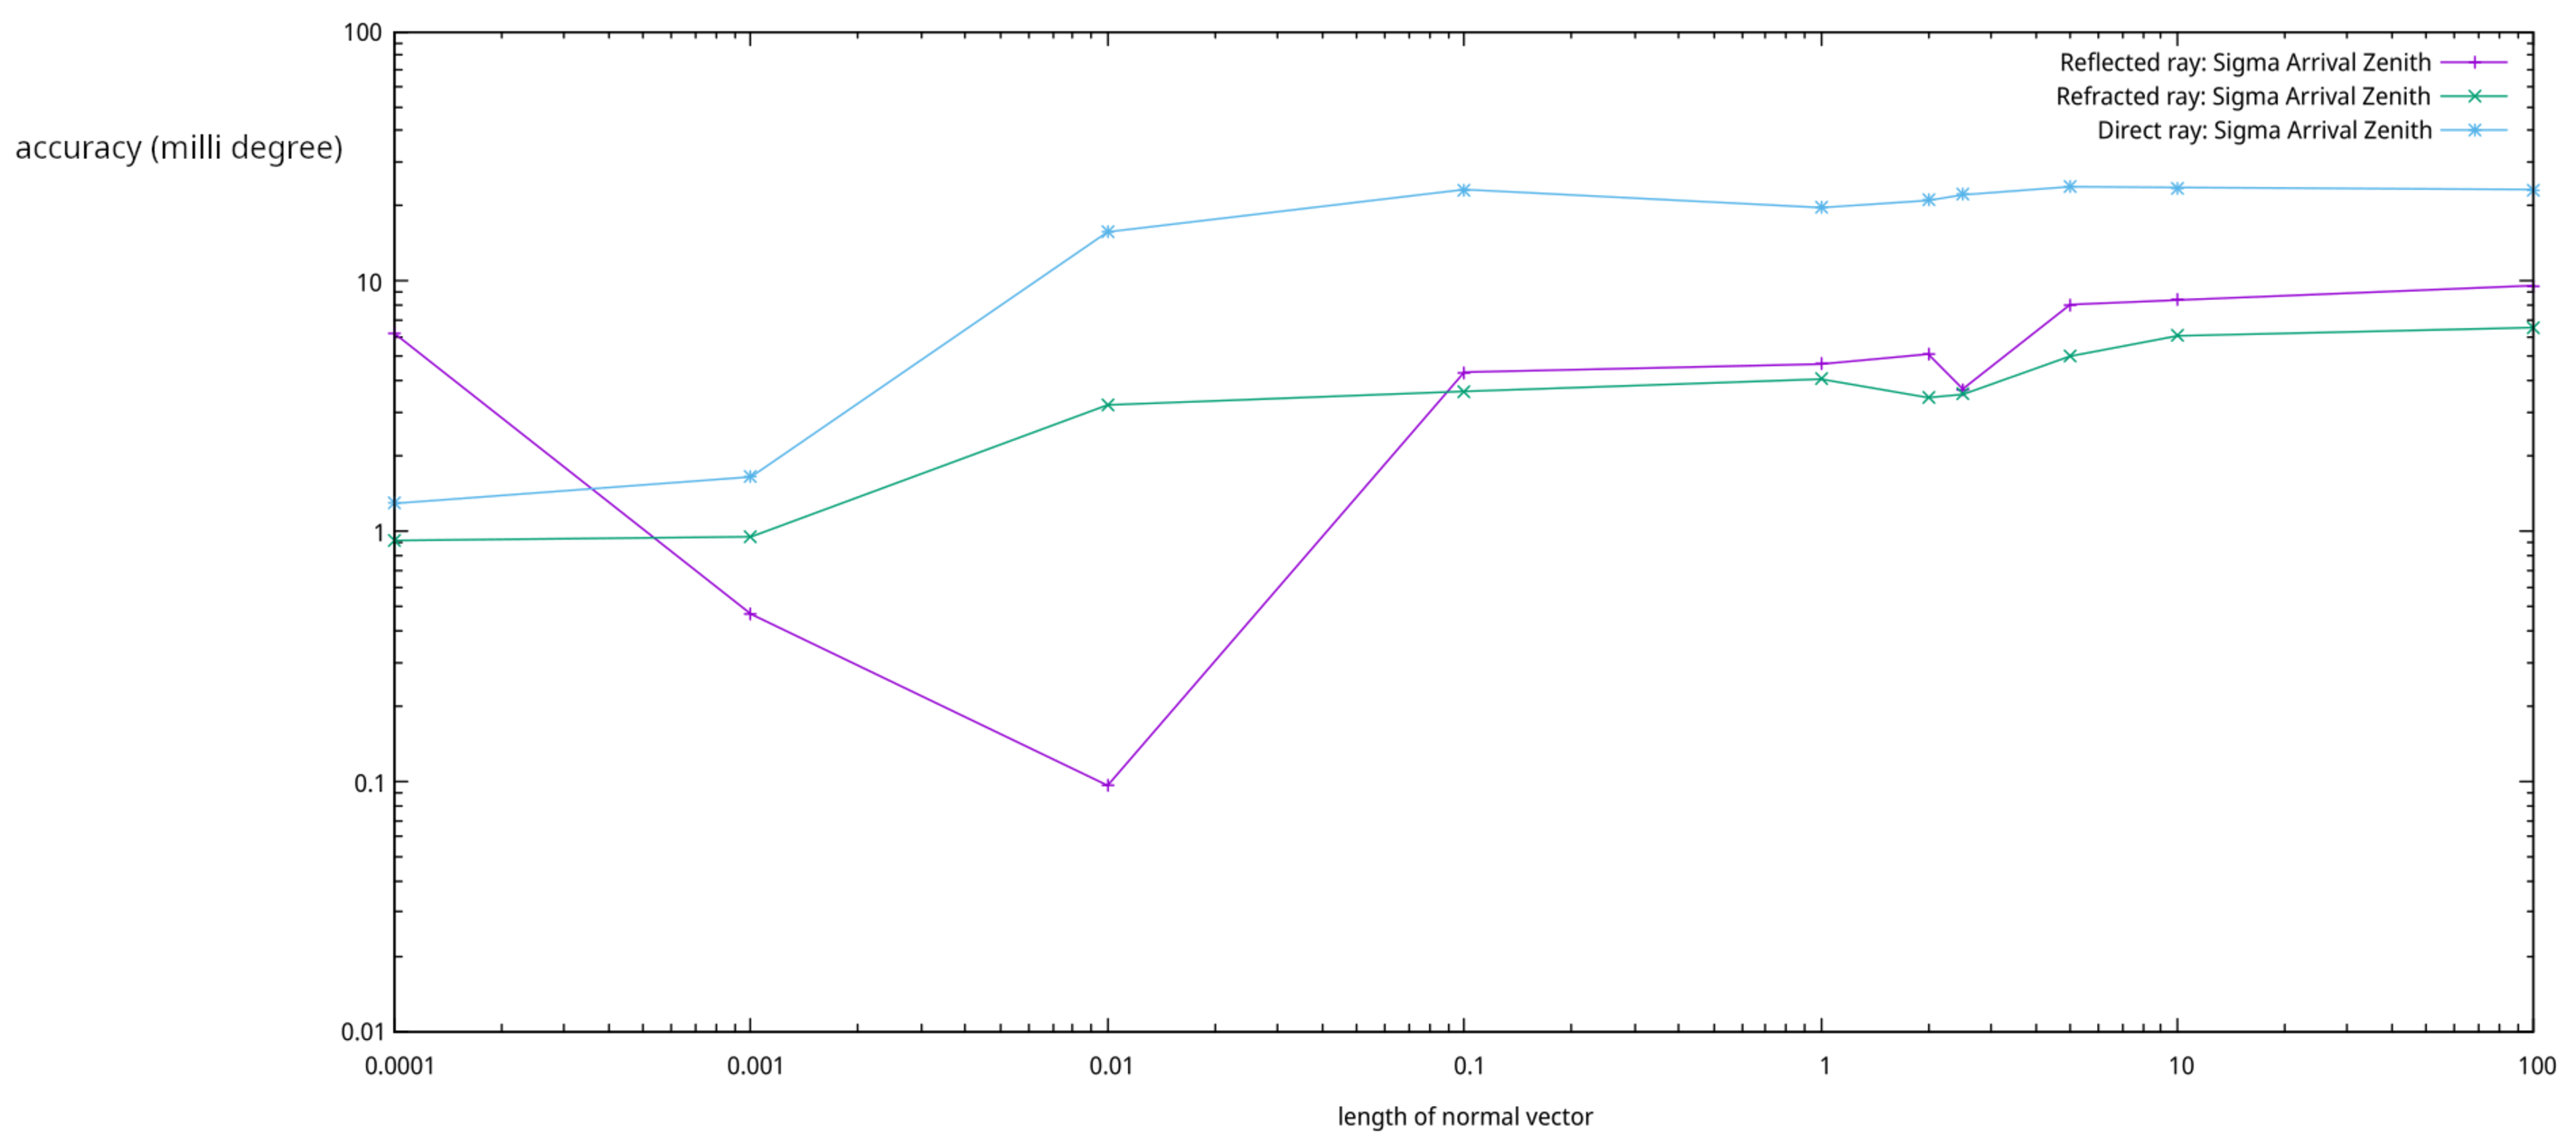
\includegraphics[width=0.8\textwidth]{figures/NormVsSigmaAZ.pdf}
	\end{minipage}
\caption{influence of the length of the normal vector}
\label{fig:norminfl2}
\end{figure}

\subsection{ztol}
We'll now change the \textit{tolerance} on the vertical distance away from the
detector which is deemed accepted i.e in figure \ref{fig:normexpl} if $\Delta
z$ is below this threshold, the minimization procedure is stopped and the last
found answer is the accepted answer.  The results from analogous comparisons as
previously discussed are shown in figures \ref{fig:ztolinfl} and
\ref{fig:ztolinfl2}.  There seems to be a minimum at 0.05m, looking at the
accuracy for this tolerance it seems sufficient to be used.  We can thus infer
the second optimization conclusion: take ztol to be 0.05 m.
\begin{figure}
	\centering
	\begin{minipage}{\textwidth}
		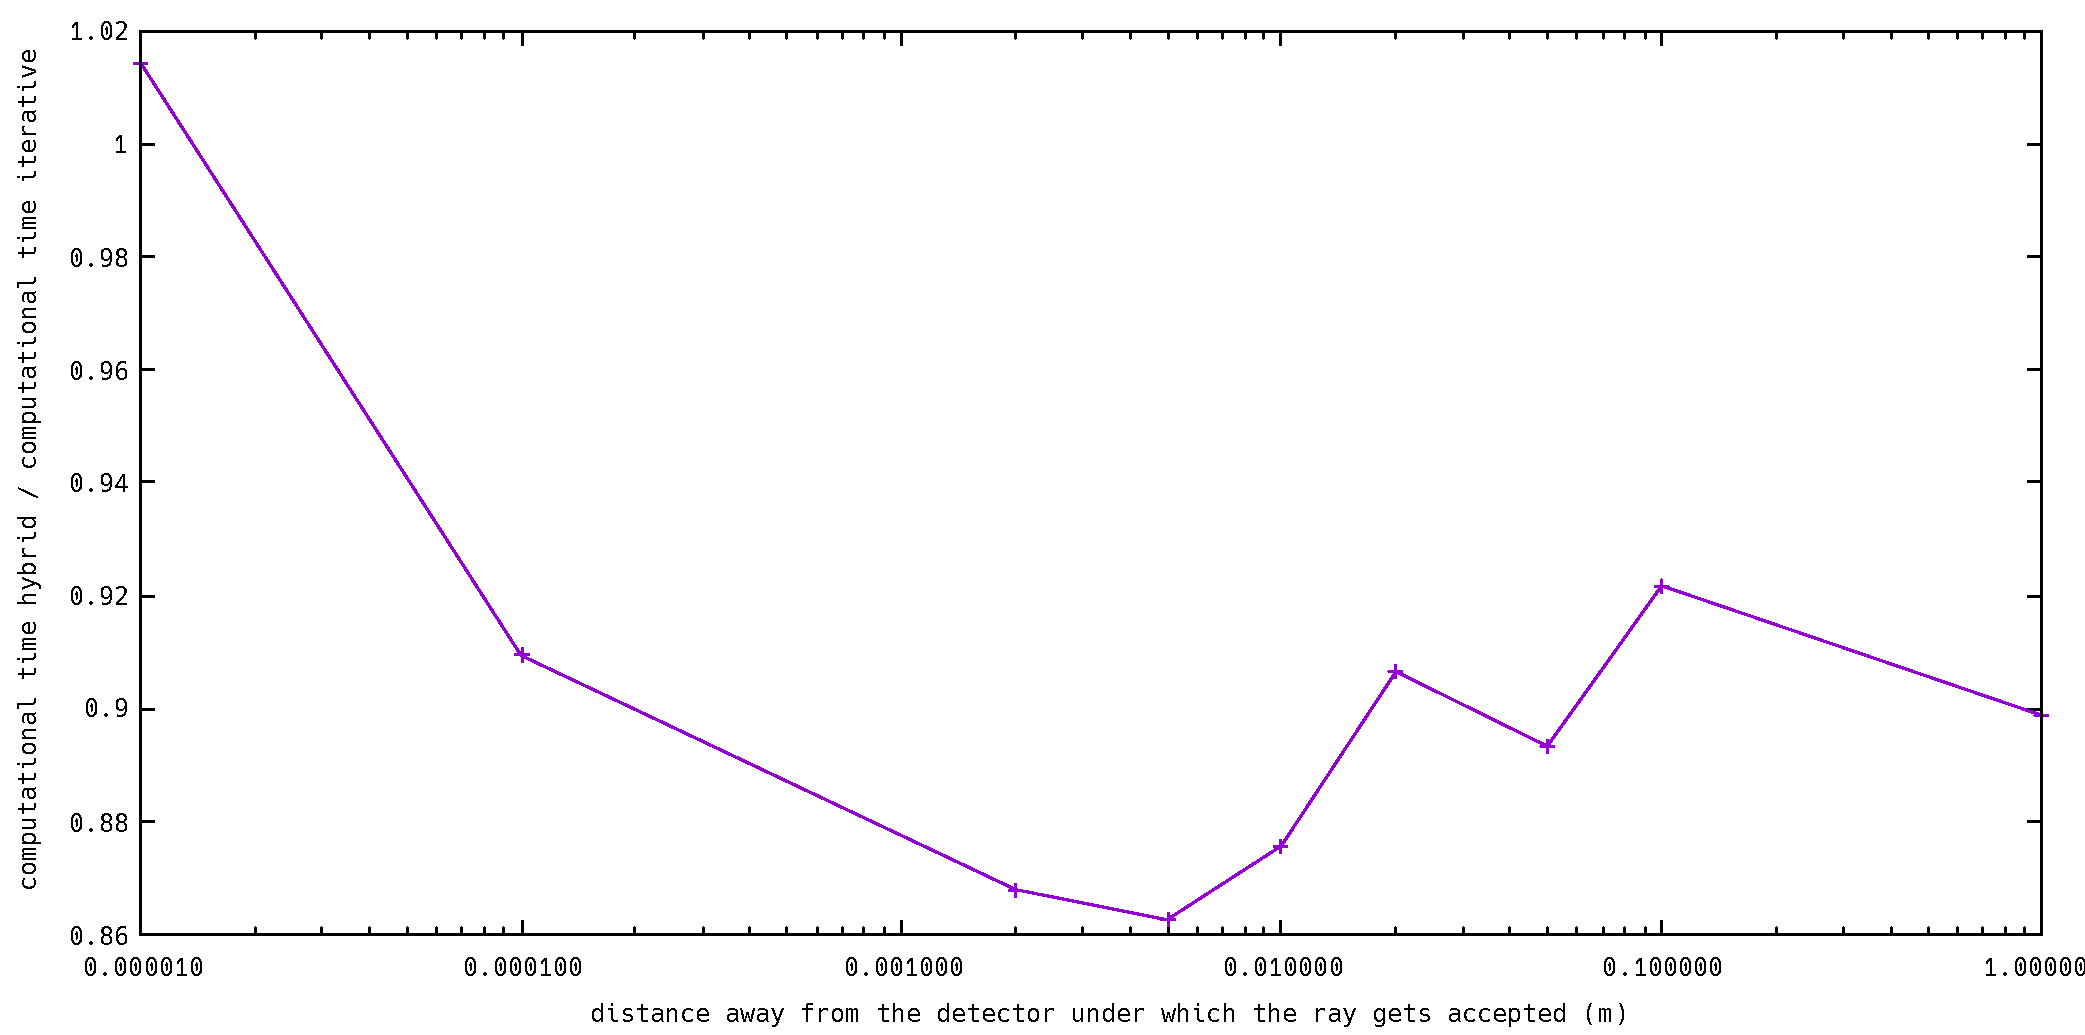
\includegraphics[width=0.8\textwidth]{figures/ZtolVsTime2.pdf}
	\end{minipage}
	\begin{minipage}{\textwidth}
		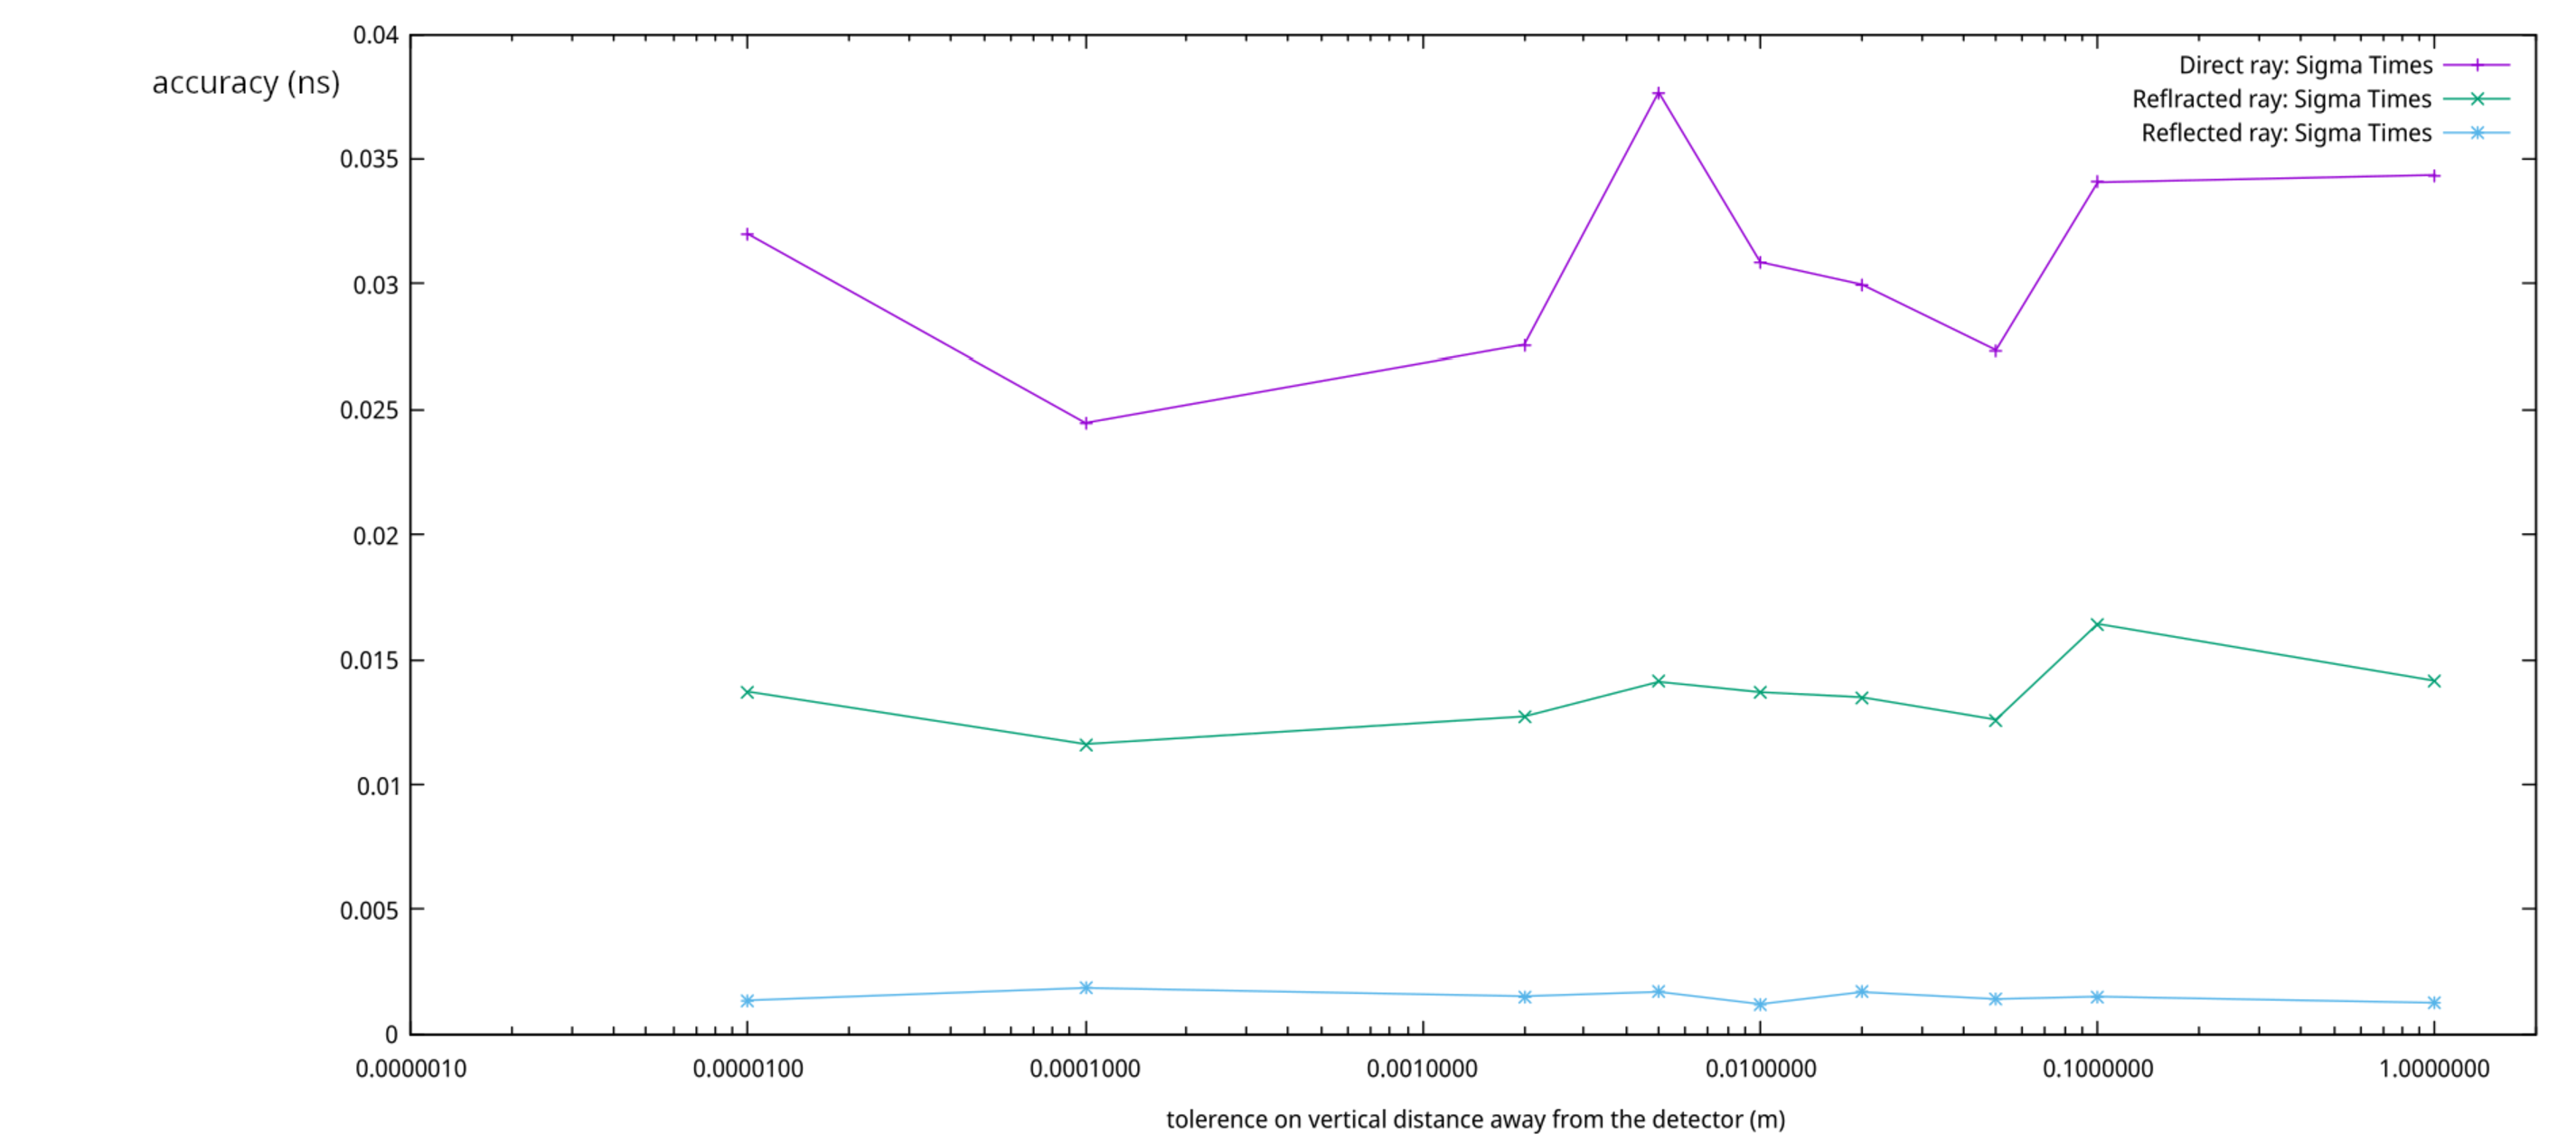
\includegraphics[width=0.8\textwidth]{figures/ZtolVsSigmaTime.pdf}
	\end{minipage}
\caption{influence of the tolerence on vertical distance}
\label{fig:ztolinfl}
\end{figure}

\begin{figure}
	\centering
	\begin{minipage}{\textwidth}
		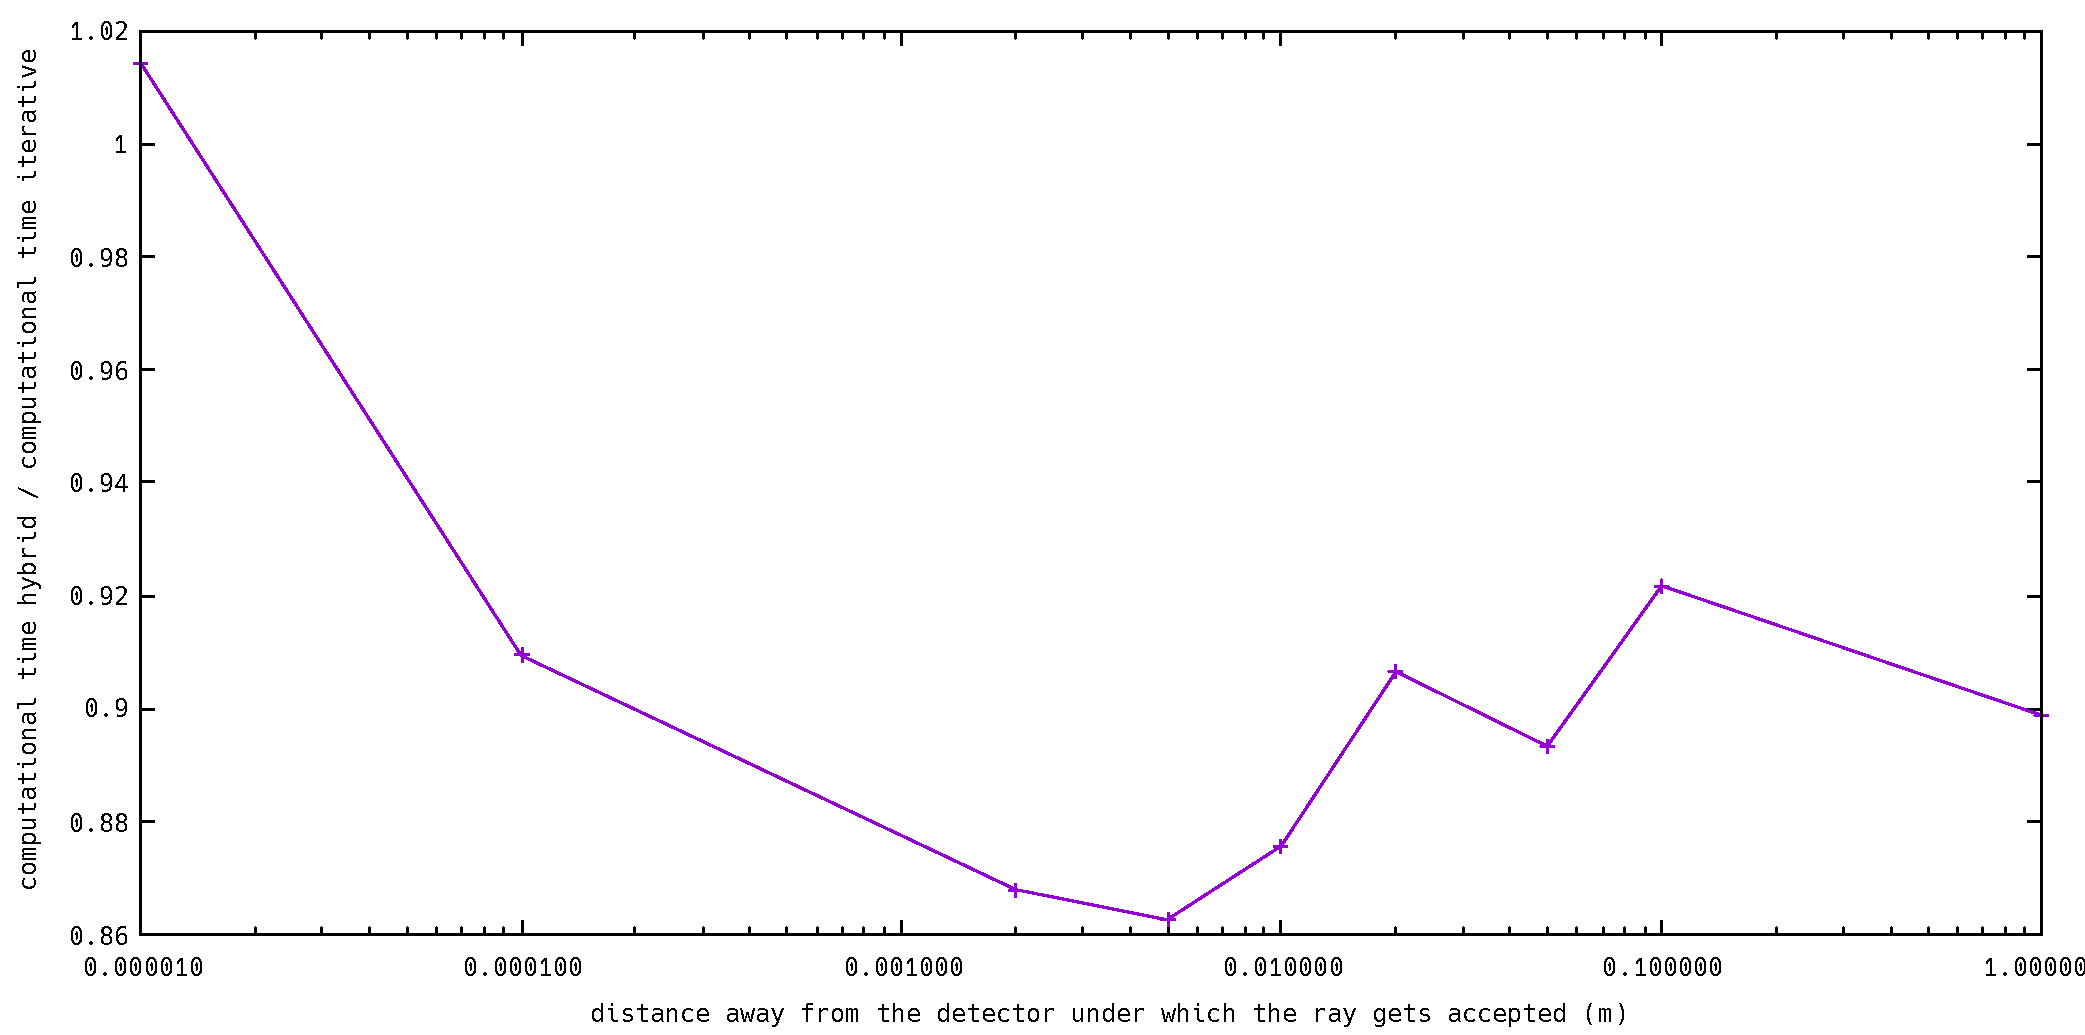
\includegraphics[width=0.8\textwidth]{figures/ZtolVsTime2.pdf}
	\end{minipage}
	\begin{minipage}{\textwidth}
		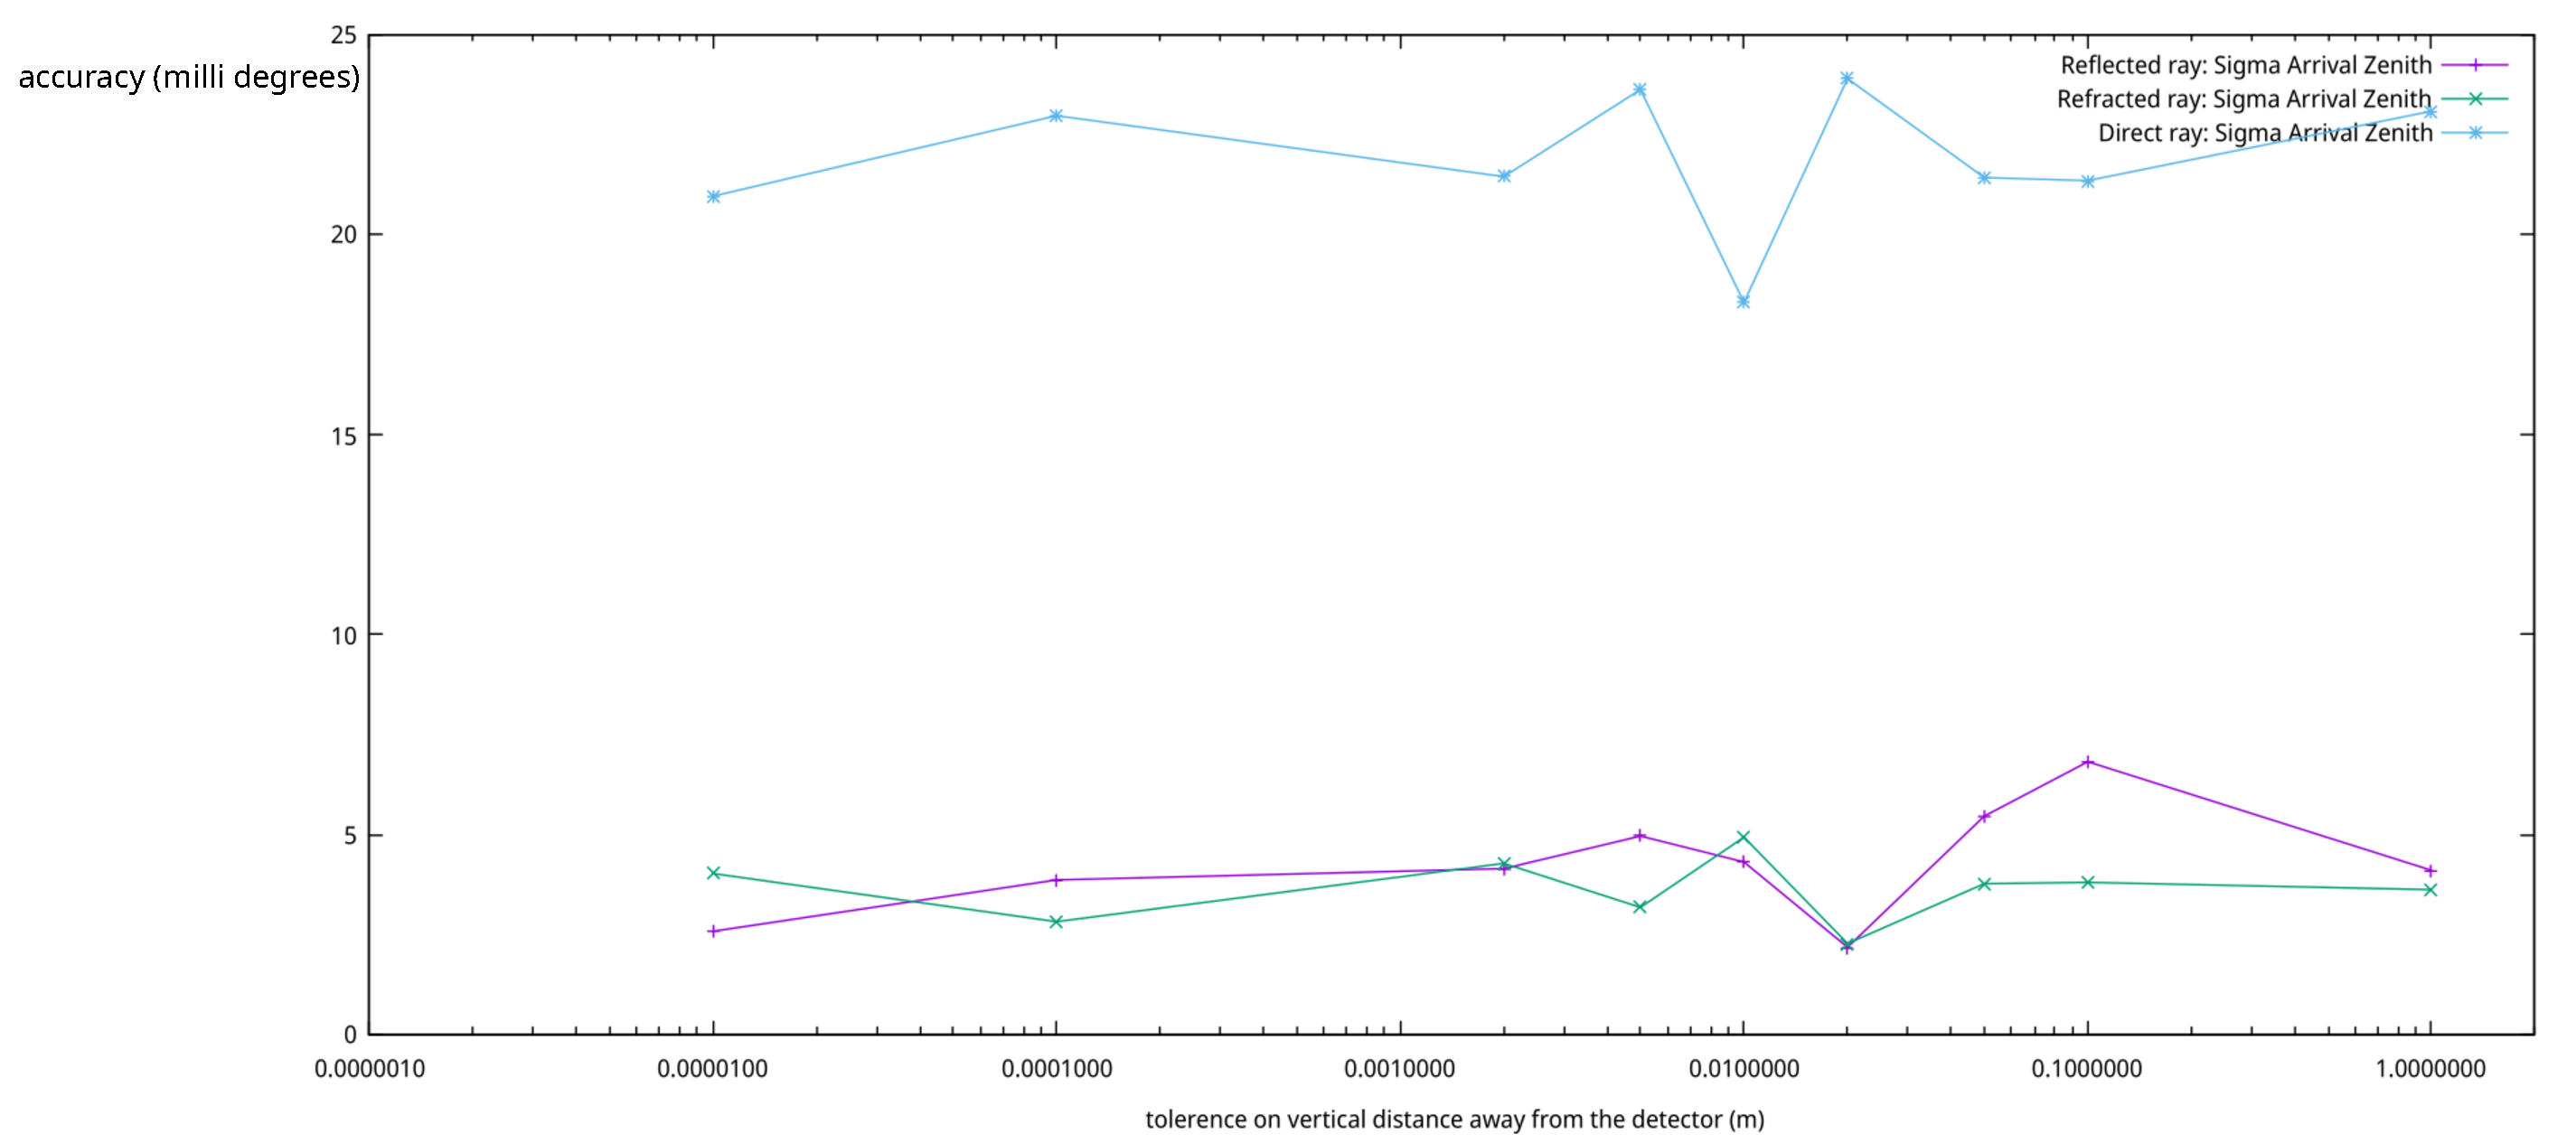
\includegraphics[width=0.8\textwidth]{figures/ZtolVsSigmaAZ.pdf}
	\end{minipage}
\caption{influence of the tolerence on vertical distance}
\label{fig:ztolinfl2}
\end{figure}

\subsection{Sphere Size \& Step Size}
The initial rays are sent out in steps of a certain angle and with a sphere
around the detector of a certain size, varying this first step of the algorithm
might thus have an effect on both the accuracy and the computational time. 
As this initial search for launch angle
regions is also the slowest step in the hybrid ray tracer it's also the most important
step to optimize. The optimization procedure is as follows: change the sphere size and loop over various
step sizes, recording the speed. Note that, as we have to vary 2 parameters, we can't really look at accuracy 
here. This isn't needed however as we'll see that after finding the optimal solution the accuracy is still superb,
apart from one part where it is needed: \textbf{if insufficient solutions are found}, as we wish this algorithm to
best the iterative ray tracer, it'll need to at least find as many solutions as the iterative ray tracer does. 
If, for a particular random interaction vertex location, less solutions are found by the hybrid ray tracer
than for the iterative ray tracer, this parameter choice will be thrown away (and colored differently).
The results of going through this are shown in figure \ref{fig:SphereStepInfl}, the points colored red 
are inusable as previously discussed.

The lower on the graph the points lie, the better. If we combine all the green points into a single plot
we get what is shown on figure \ref{fig:SphereStepFinal},
zooming in onto the lowest point , we see that an optimal sphere size seems to be at 45m accompanied
by a stepsize of 0.7°.
\begin{figure}
	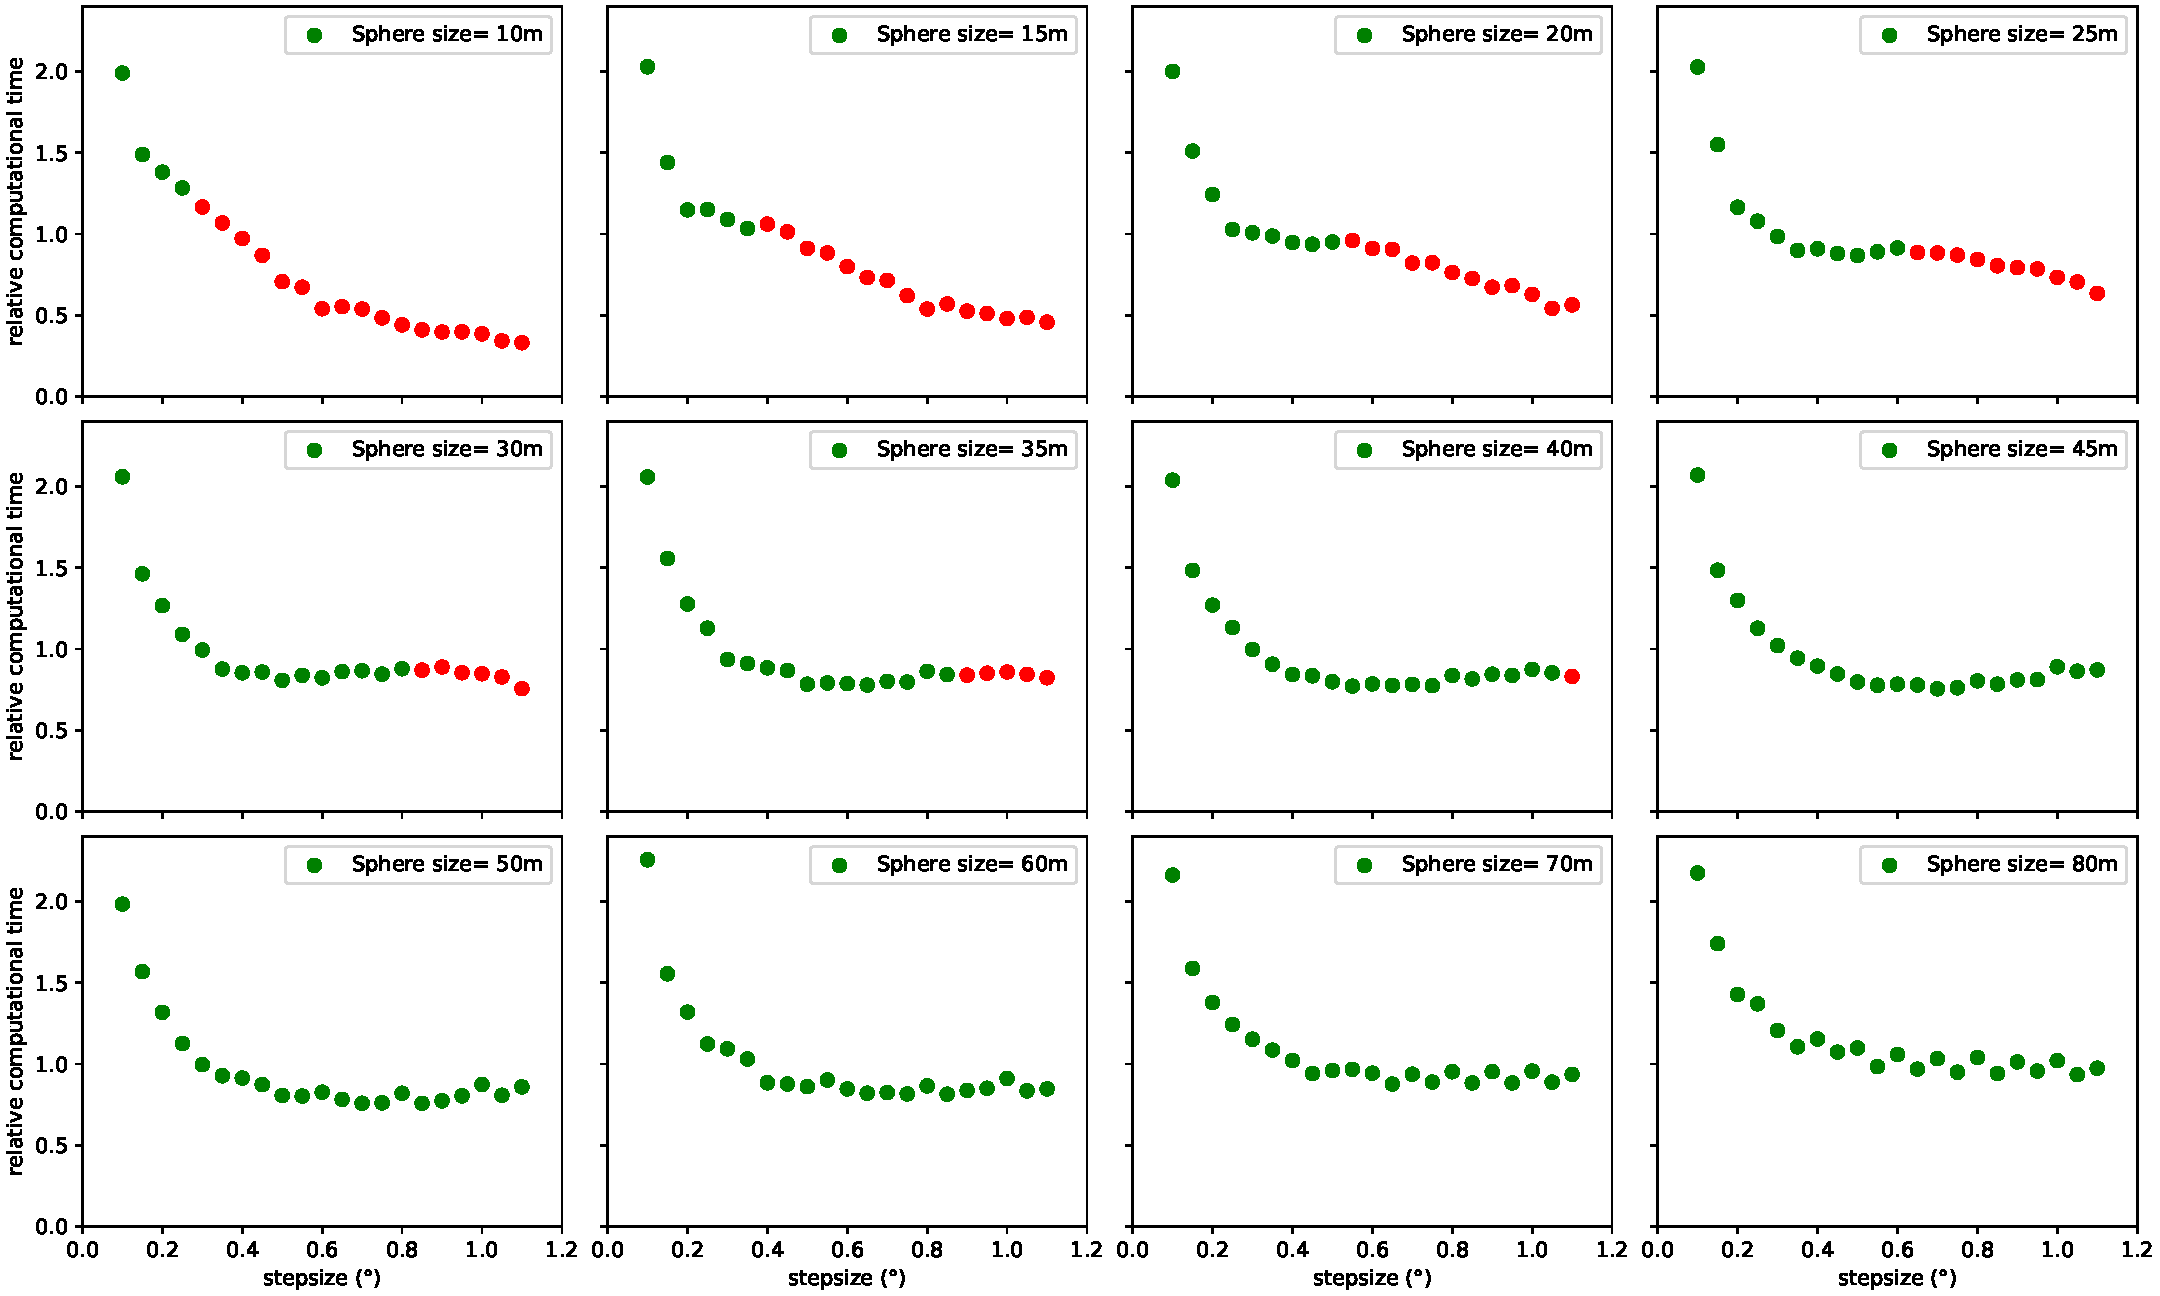
\includegraphics[width=\textwidth]{figures/subplotofallstepsphere.pdf}
	\caption{Variation in Sphere and angle step size with report on relative time.}
	\label{fig:SphereStepInfl}
\end{figure}
\begin{figure}
	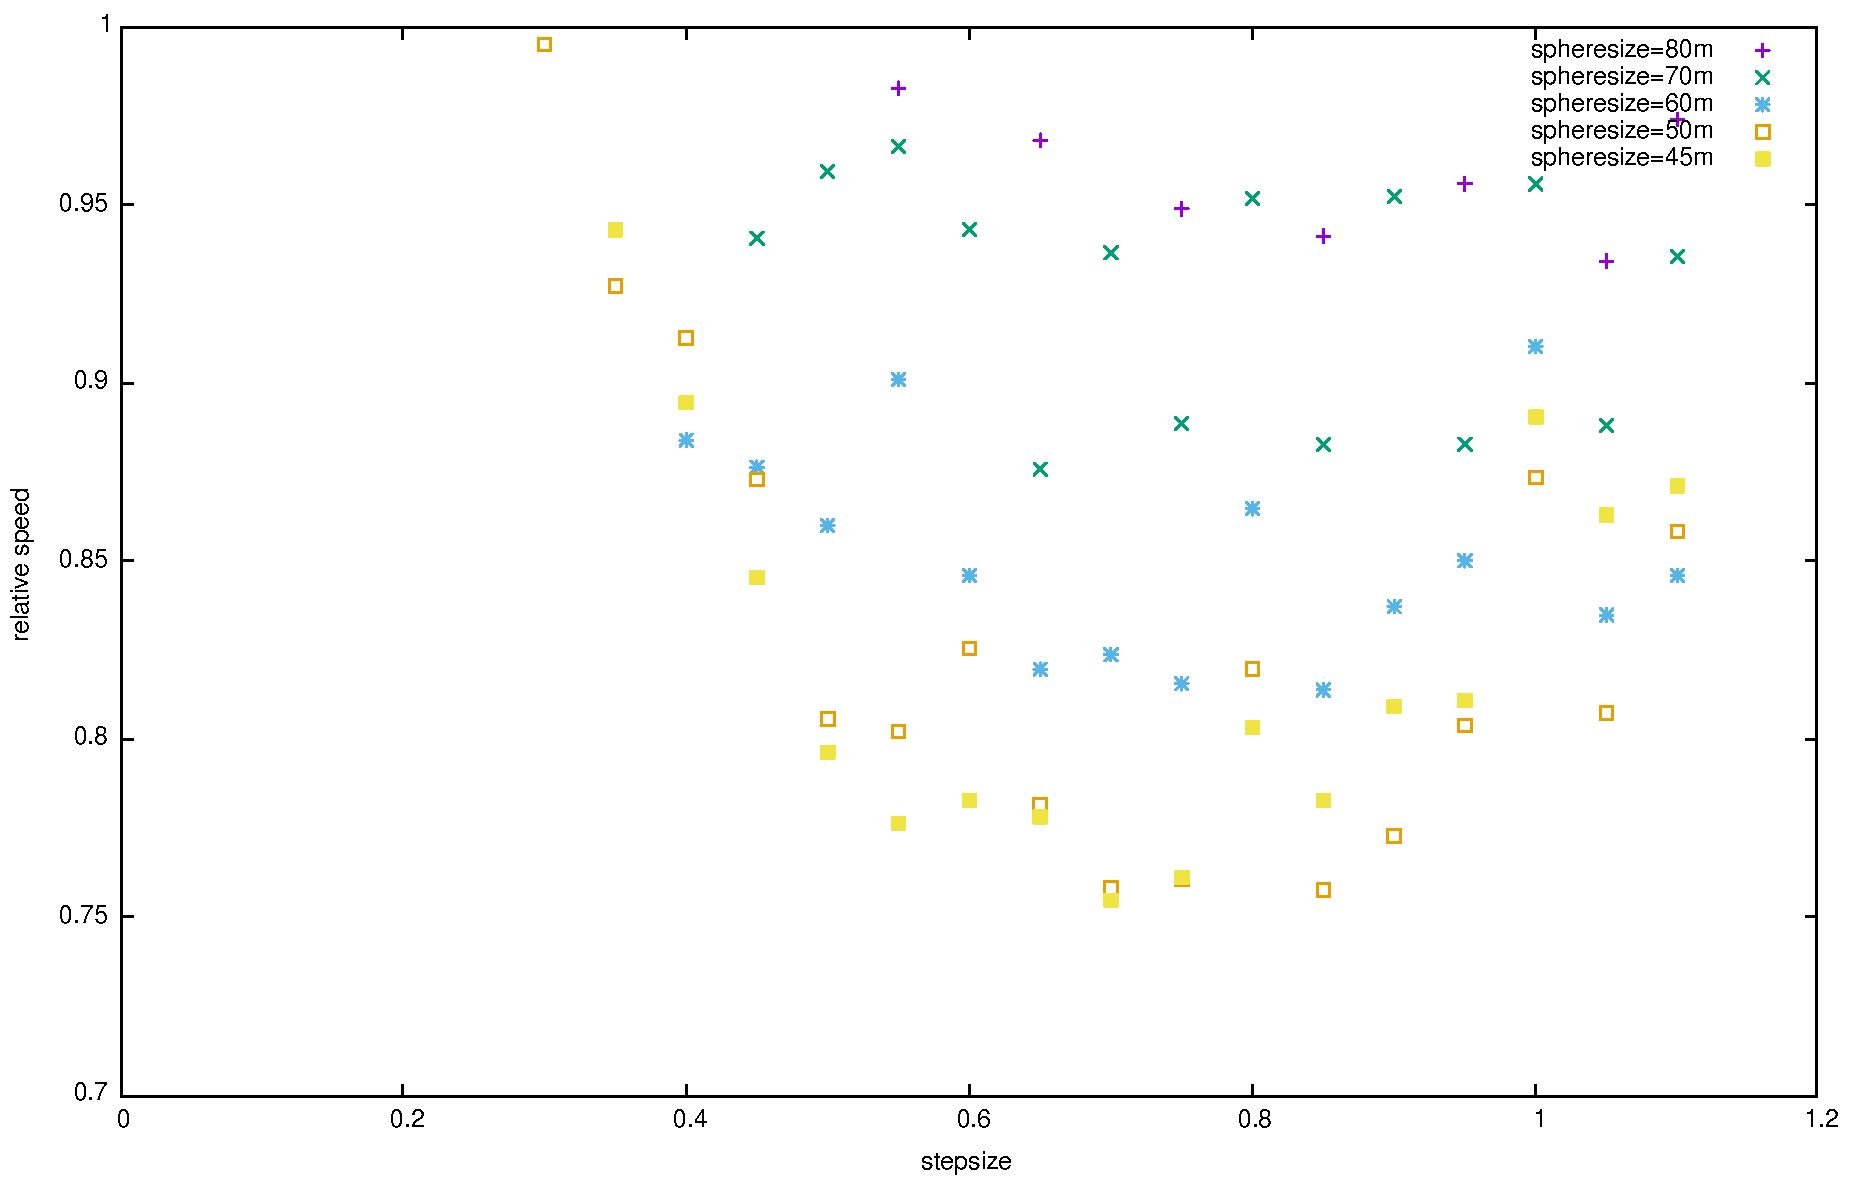
\includegraphics[width=\textwidth]{figures/SphereAndStepFinal.pdf}
	\caption{Green values in variation in sphere and angle step size with report on relative time.}
	\label{fig:SphereStepFinal}
\end{figure}
\newpage
\subsection{Conclusion of optimization}
How does the hybrid ray tracer perform relative to the iterative ray tracer if we use 
the previously optimized variables? After doing a simulation of 1000 random source locations with
the iterative, analytic and hybrid ray tracer and comparing both the iterative to the analytic and the hybrid to the analytic
we get what's shown in figures \ref{fig:acchyb} and \ref{fig:accit}. Where we can clearly see that the hybrid
ray tracer is more accurate, now during this simulation we also recorded the computational speed, the results
are presented below:
\begin{itemize}
	\item iterative: 0.61 computations/s
	\item hybrid: 0.82 computations/s
	\item analytic (c++ compiled version): 10289 computations/s
\end{itemize}
The hybrid ray tracer is thus 33.7\% faster than the iterative ray tracer, the speed of the analytic ray tracer
has a difference to the other two that might seem quite overwhelming but this might get mitigated in the future if 
part of the hybrid ray tracer gets re-written in a compiled language (like c++).

\begin{figure*}
	\centering
\begin{minipage}{0.49\textwidth}
	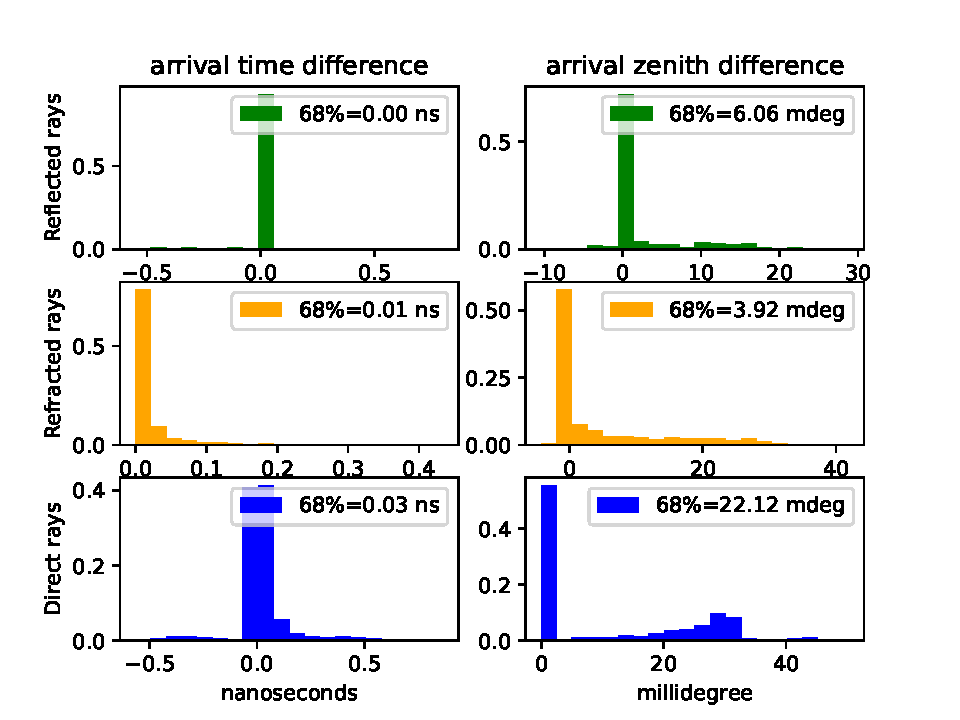
\includegraphics[width=1.1\textwidth]{figures/hybrid_comparison_N_1000.pdf}
	\caption{Hybrid}
	\label{fig:acchyb}
\end{minipage}
\begin{minipage}{0.49\textwidth}
	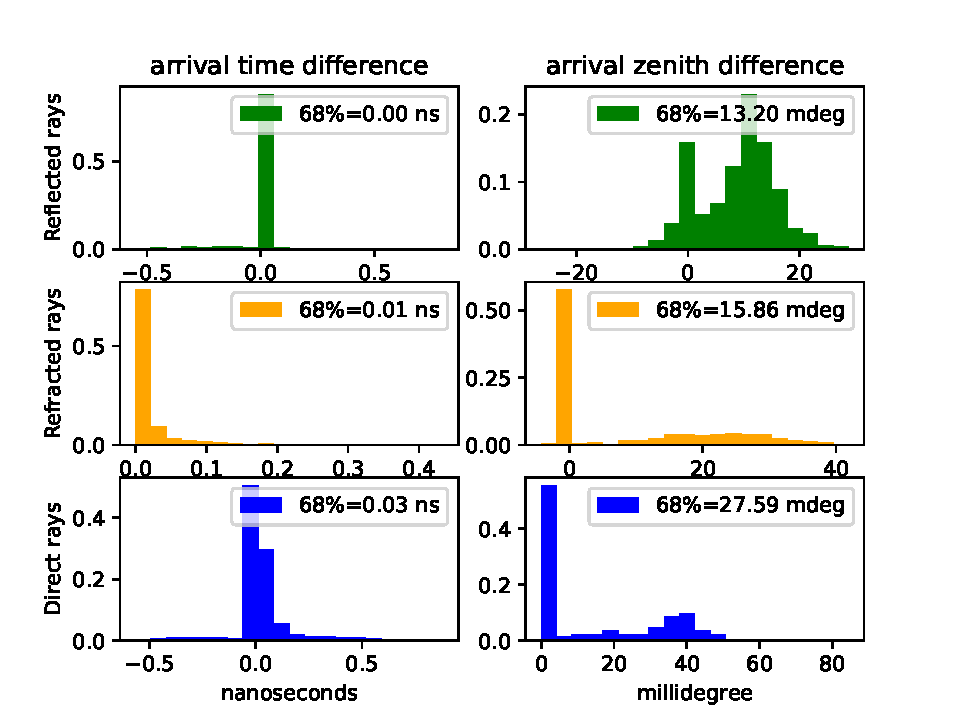
\includegraphics[width=1.1\textwidth]{figures/iterative_comparison_N_1000.pdf}
	\caption{Iterative}
	\label{fig:accit}
\end{minipage}
\end{figure*}

\section{Expansion}
Using the ray tracer as it is now defined makes us unable to calculate paths by \textit{secondaries}.
When your ice model has some kind of added complexity like a reflective bottom or a discontinuity layer 
(like what will be the case for our air-bourne balloon in the next chapter)
you'll need to account for secondaries, these are additional rays like an extra refracted or reflected rays that get generated at this discontinuity. How the algorithm is now it will follow one ray from the source to the discontinuity and 
only consider say the reflected ray, whilst a refracted ray generated at such a discontinuity might actually end
up closer to the detector.

To implement secondaries, we'll just check if there are any found at the delta\_z algorithm and if so loop over them,
keeping the original ray's $\Delta z$ in mind as the "global best" and looking if any of the secondary rays' $\Delta z$ is 
lower than the "global best" if so this will be considered the new final ray which gets returned and the $\Delta z$ that
gets returned is the new "global best" originating from the secondary, if there is no secondary ending closer than the "original" ray than the original ray with it's $\Delta z$ is returned.

\chapter{Weather Balloon}
\label{chap:WB}
In this chapter we'll infer information about the ice the detectors reside in
using radio signals coming from a weather balloon flying over the stations. 
We'll go about this by first finding the difference in timing between  
channels by fitting the balloon's sinusoidal signal to the data, and
then doing a plane wave reconstruction for different indices of refraction
until we find one where the reconstructed signal gets close to the balloon.
This procedure will be explained more in depth over the following sections.

For us to find the timing we'll first make an educated guess, this can be done
using our \textit{hybrid minimizer} algorithm, there is one change that need to
happen first to our algorithm for us to be able to simulate this: The air
observers needs to be hard removed as to make a ray tracing possible from
within the air into the ice and onto the detector.

Due to the way our algorithm works the time the ray took is only from when it
became a secondary\footnote{This might get fixed in the future but as
secondaries weren't needed for most applications we deemed it fine for the
moment}, this information is insufficient as we want the full travel time.  The
propagation time from the balloon to the ice $t$ can later be added to the time
of the path in the ice by measuring the length $d$ of the drawn line from the
balloon to the beginning of the recorded path, setting the speed of radio waves
in air to the speed of light c and then just adding $t = d/c$ to the time found
from the algorithm.
\section{Plane Wave Reconstruction}
Now having modified our ray tracer, the first problem we'll consider is
plane wave reconstruction of the original position, an example path
to some of the deep sensors is given in figure \ref{fig:Example
trajectory}
\begin{figure}
	\centering
	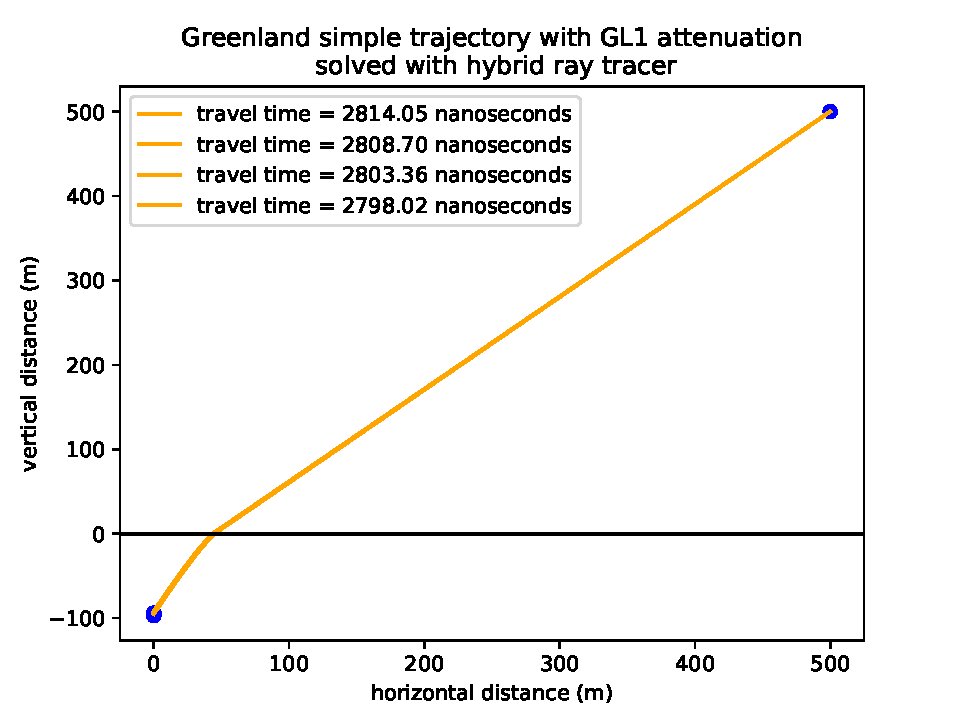
\includegraphics[width=0.7\textwidth]{weerballontraject.pdf}
	\caption{Example trajectory of rays coming from a weather balloon (blue dot top right) and going through the ice to the various detectors (blue dots bottom left)}
	\label{fig:Example trajectory}
\end{figure}
\begin{figure}
	\centering
	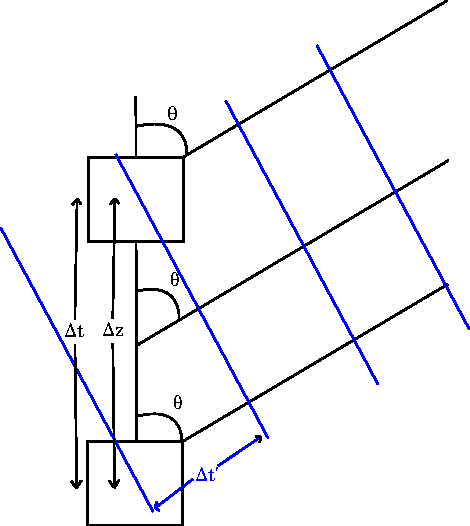
\includegraphics[width=0.7\textwidth]{planewave.pdf}
	\caption{Illustration of Plane waves}	
	\label{fig:Plane Wave}
\end{figure}
The plane wave reconstruction can easily be understood using figure
\ref{fig:Plane Wave}, the radio waves coming from the weather balloon are drawn
in blue and make a certain angle with the detectors. the top detector (top box)
detects the wave at a certain time $t_1$, the bottom detector detects it at a
time $t_2$. In our database, after decoding the signal we'd thus see that these
two detectors got a signal $\Delta t = t_1 - t_2$ seconds apart from eachother.
Now ideally this is equal to the time $\Delta t'$ which is the time it took the
wave to propagate that distance which we can calculate from basic trigonometry
and dimensional analysis:
\begin{equation}
	\Delta t' = \frac{m}{(m/s)} = (s/m)*m = v^{-1} * m = v^{-1} \cos\theta \Delta z
	\label{eqn:deltataccent}
\end{equation}
With $v = c/n$ the local speed of light and n the index of refraction at the depth inbetween
the considered channels. 
Thus if we know the angle $\theta$, the time $\Delta t'$ and the distance between the channels $\Delta z$
we could infer the index of refraction at a certain depth as can be seen by reforming equation \ref{eqn:deltataccent}:
\begin{equation}
	n = \frac{\Delta t'}{\Delta z} \frac{c}{\cos\theta}
	\label{eqn:deltataccent}
\end{equation}
%\begin{mintedbox}{python}
%ice = medium.greenland_simple()
%n_exact = ice.get_index_of_refraction(np.array[0,0,-95.5])
%\end{mintedbox}
In reality we don't know the angle a priori, we'll only have the recorded
timing information $\Delta t$ and the difference in channel height $\Delta z$.
So to this end we'll perform a scan by choosing some index of refraction $n_1$ and
minimizing the \textit{correlation function}:
\begin{equation}
	Correlation(\theta) := \Delta t - \Delta t' = \Delta t
	- \frac{\cos\theta \Delta z}{v}
  \label{eqn:PlaneWave}
\end{equation}
If we want to use more than 2 detectors at once however (which can be done in
the case of RNO-G), we'll need to specifiy various correlation functions.  E.g
if we have four detectors labeled 0 to 3 we'll have to construct correlation
functions between detectors 0\&1, 0\&2, 0\&3, 1\&2, 1\&3 and 2\&3 .  As all of
these correlation functions will have different sizes we'll norm them as
follows:
\begin{equation}
	Correlation_{Normed}(\theta) =
	\frac{Correlation(\theta)}{\int Correlation(\theta)\Delta
	\theta}
\end{equation}
An example of these correlation functions is shown in figure \ref{fig:NormedCorrelation}, 
notice how you can't differentiate between the correlation functions, this is only possible
because of the hybrid ray tracer having that high of a precision.
\begin{figure}
	\centering
	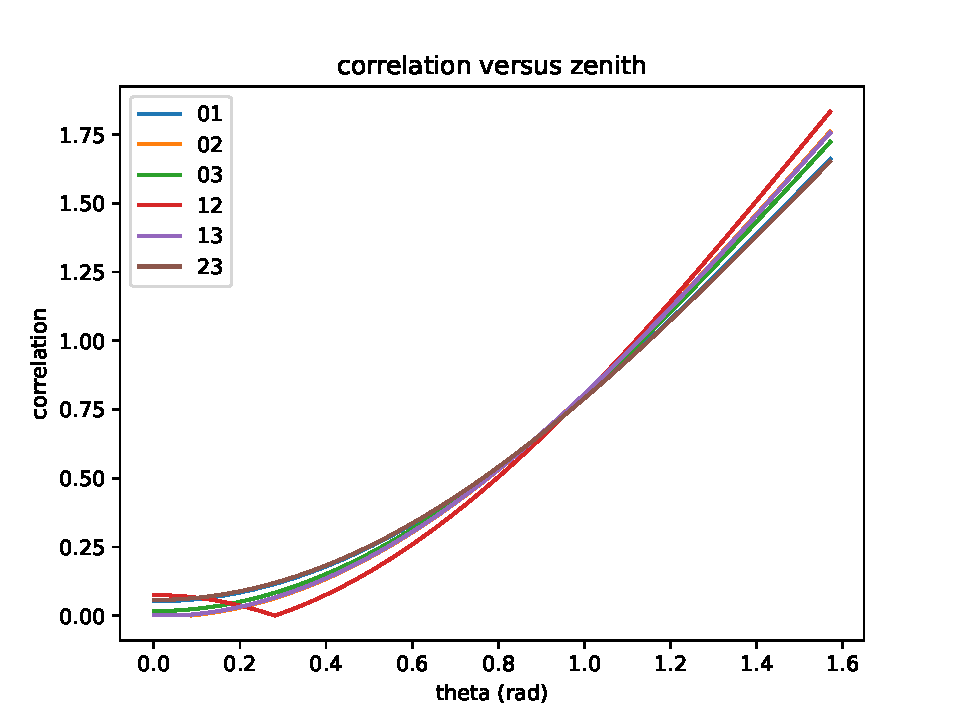
\includegraphics[width=0.8\textwidth]{NormedCorrelation.pdf}
	\caption{Example normed correlation functions}
	\label{fig:NormedCorrelation}
\end{figure}
\begin{figure}
	\centering
	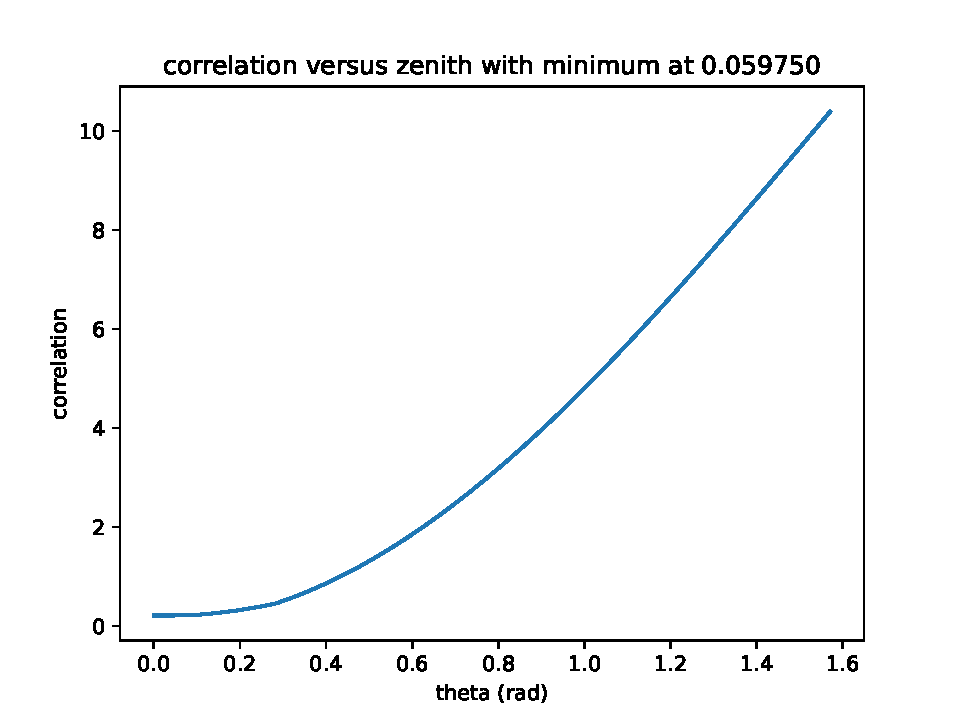
\includegraphics[width=0.8\textwidth]{SummedCorrelation.pdf}
	\caption{Example sum of the normed correlation functions}
	\label{fig:SummedCorrelation}
\end{figure}
After this we can sum them, as shown in figure \ref{fig:SummedCorrelation}, and look
at which angle it reaches it's minimum. Using this angle we can then reconstruct a ray and guess 
where the weather balloon is approximately, this is illustrated in figure 
\ref{fig:WeatherBalloonPositionReconstruction}. 
\begin{figure}
	\centering
	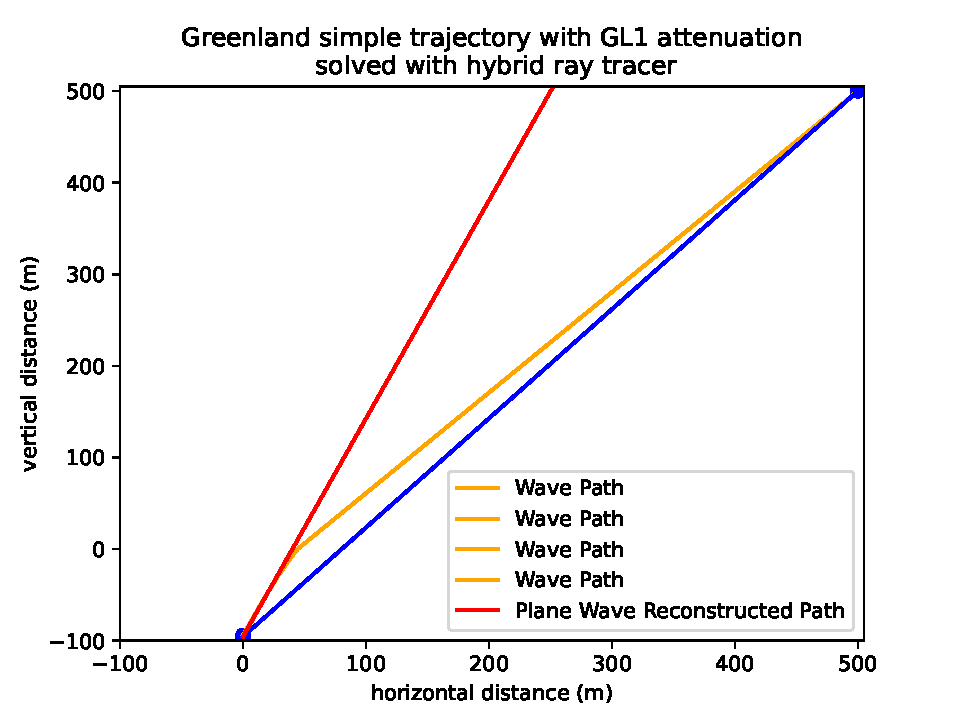
\includegraphics[width=0.7\textwidth]{WeatherBalloonPositionReconstruction.pdf}
	\caption{Example plane wave reconstruction of weather balloon position}
	\label{fig:WeatherBalloonPositionReconstruction}
\end{figure}
We can calculate the difference in distance between the weather balloon and the plane wave at the same height
and label this $d_1$, then we can choose another index of refraction $n_2$ which again corresponds to a difference
$d_2$ and so forth. At the end we take the index of refraction $n_i$ which corresponds to the minimal distance $d_i$
as the fitted index of refraction.

\section{Is the goal feasible?}
\subsection{No assumptions}
In the example reconstruction illustrated in figure
\ref{fig:WeatherBalloonPositionReconstruction} the difference in angle between
direct to balloon and plane wave reconstruction is already quite small
(0.65329617\%) but as the balloon gets closer to the detector this reduces
significantly. As previously layed out, our goal is to find the local index of refraction n by using the
plane wave reconstruction with the recorded timing and the positional data from
the weather balloon.

Now let's ask ourselves the question, within which angles should the
weather balloon fly for the data to be useful?  As was previously stated, the
further the weather balloon is away (in the x direction) the bigger the zenith
angle with the detector the less accurate the plane wave reconstruction.  So
which angles are acceptable? Note that not only angle but also height will eventually
play a role in the accuracy, the angle however gives a good starting point.
To determine this our method works as follows: 

We vary the position of the weather balloon in the x direction (keeping the
height constant at 500m), simulate the ray path to the channels 0 to 3 and then fit n
such that the difference between the balloon position and the plane wave at the same
height is as small as possible.  Then we compare the n we have fit to the
one we know from the model at that position.  We quantise the discrepency
between these two indices of refraction using what we here define as the
\textit{relative accuracy}:
\begin{equation}
  \varepsilon\ (\%) = \frac{n_\text{fit} - n_{\text{exact}}}{n_{\text{exact}}} \times 100
\end{equation}
Carrying this out\footnote{The code for this can be found in projects-mt/BaLLooN/simulations as plane\_wave.py} we get figure \ref{fig:EpsilonIFODirect}, i.e it gets
exponentially shifted towards higher n as the balloon moves further away. If we wish our
accuracy to be within 1\%, the angle the balloon makes with the middle of channels 0 to 3 needs
to be less than 10°.
\begin{figure}
	\centering
	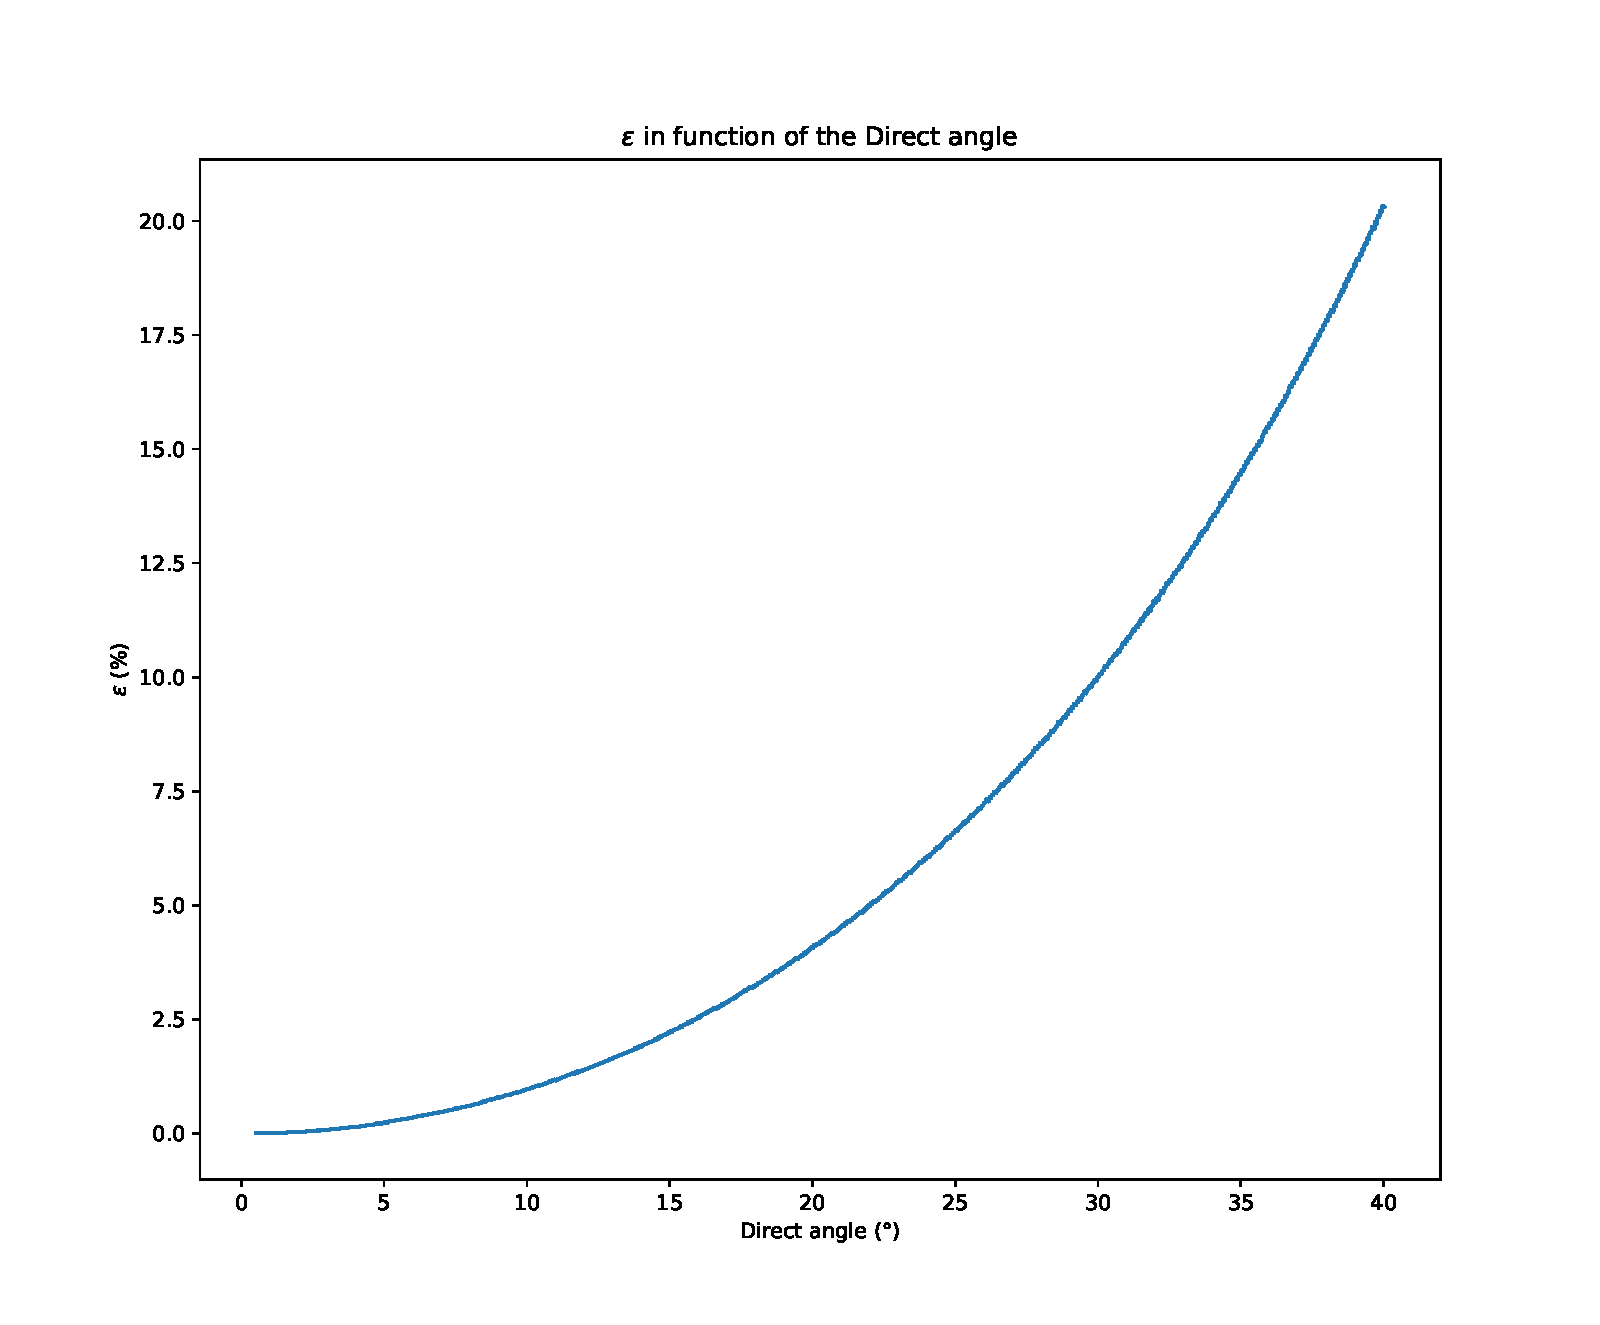
\includegraphics[width=0.7\textwidth]{EpsilonIFODirect.pdf}
	\caption{Epsilon in function of the direct angle}
	\label{fig:EpsilonIFODirect}
\end{figure}
Now what would our $<$10° policy entail? And is it even possible?  Say we take
a look at station Terianniaq (station 12) and see what our policy entails,
it is located at 72.6000868058195° N -38.4962265332872° W in the global geographic
coordinate system (longitudinal, latidude and elevation), this is quite
difficult to work with directly. For this reason we first convert the station's location to 
local ENU coordinates (east, north, up) relative to the the 'DISC' which is a point in the base camp located at
72.58279265212887 latitude, -38.45581495328228 longitude and 3251.9489147560234 elevation.  

After having converted station 12's position into ENU coordinates we get
-137.67250176003688N 1727.5184983294744E, we then set our "up" to be -95.5m as
this is the approximate location of the middle of channels 0-3.  Now looking at
e.g the Balloon path recorded on the 20th of august 2022 (figure
\ref{fig:ExampleBalloonPathCrossing12}) we see that the balloon crosses paths
closely with detector 12, but how close was this encounter? To quantize this we
can take a look at every balloon positional data entry (there are $>$12000
entries) individually and compute the angle the balloon makes with the detector
by first converting the location of the balloon into ENU coordinates, then
calculating the lateral distance ($\sqrt{(x-x')^2 + (y-y')^2}$) then the
relative vertical distance $|z - z'|$ and then from those compute the angle
($\tan(\theta) = \frac{Hor.}{Vert.}$) doing this and recording when the balloon
gets close enough to get below the 10° mark we get the yellow part of figure
\ref{fig:ExampleBalloonPathCrossing12}. We thus see that in this
example the $<10$° policy is viable.

Now how much data do we have that way? 
We'll be looking at the data recorded over the summer of
2022, more particularly 15/06/2022 - 30/09/2022.
The positional data of the weather balloons was obtained from the
\url{ftp1.esrl.noaa.gov} website using the rno-g-sonde script of the official
RNO-G github page. After looping through every weather
balloon gpx file recorded in the summer of 2022 and seeing when it gets
within 10 degrees from any detector we get the data shown in appendix \ref{app:10Deg}, even
though this is quite a lot of data there's still another step that we could do
to broaden the amount of usable data.
\subsection{Refraction at the surface}
Up until now we have not used the property that waves refract at the surface as
we didn't want to assume anything, now say that we include refraction at the
surface for our plane wave reconstruction. This would mean that we'd follow
analogous steps as our previous analysis, i.e doing a plane wave reconstruction
from the difference in timing and trying to fit the index of refraction, only
now the plane wave abides with snell's law at the surface, going from n=1.27 to
n=1. 

The full algorithm thus goes as follows: We first reconstruct the
plane wave launch angle $\theta_1$ by minimizing the correlation function
previously defined, we can use this angle and the height of the middle of the
concerned detectors to derive the function
\begin{equation}
	z = a_{InIce}*x + b_{InIce}
	\label{eqn:InIcePlaneWave}
\end{equation}
The outgoing zenith angle at the surface $\theta_2$ can be calculated from snell's law:
\begin{equation}
n_1 \sin{\theta_1} = n_2 \sin{\theta_2} \implies  \theta_2 = \sin^{-1}\left(\frac{n_1}{n_2}\sin{\theta_1}\right)
\end{equation}
from this we know the slope of the wave path $a_{InAir} = \tan\left({\frac{\pi}{2} -
\theta_2}\right)$ but not the offset, but this can easily be found from equation
\ref{eqn:InIcePlaneWave} as 
\begin{equation}
	z = 0 = a_{InIce}*x_{End} + b_{InIce} \implies x_{End} = -\frac{b_{InIce}}{a_{InIce}}
\end{equation}
and 
\begin{align}
	z = 0 = a_{InAir}*x_{End} + b_{InAir} \implies b_{InAir} &= -a_{InAir}*x_{End}
	\\&= a_{InAir}* \frac{b_{InIce}}{a_{InIce}}
\end{align}
Now that we have the function describing the "path of the plane wave"\footnote{we use double
quotes as to emphasize that this is a reconstruction method and not an actual wave} in the air 
we can find out the horizontal position at the height of the balloon as
\begin{equation}
	z = z_{Balloon} = a_{InAir}*x_{f} + b_{InAir} \implies x_f = \frac{z_{Balloon} - b_{InAir}}{a_{InAir}}
\end{equation}
and iteratively loop over possible indices of refraction, minimizing $|x_{Balloon} - x_f|$.

Doing this whilst looping over possible horizontal balloon positions, we get
the result shown in figure \ref{fig:EpsilonIFODirectSnell}\footnote{The code
for this can be found in projects-mt/BaLLooN/simulations as
plane\_wave\_with\_snell.py}
\begin{figure}
	\centering
	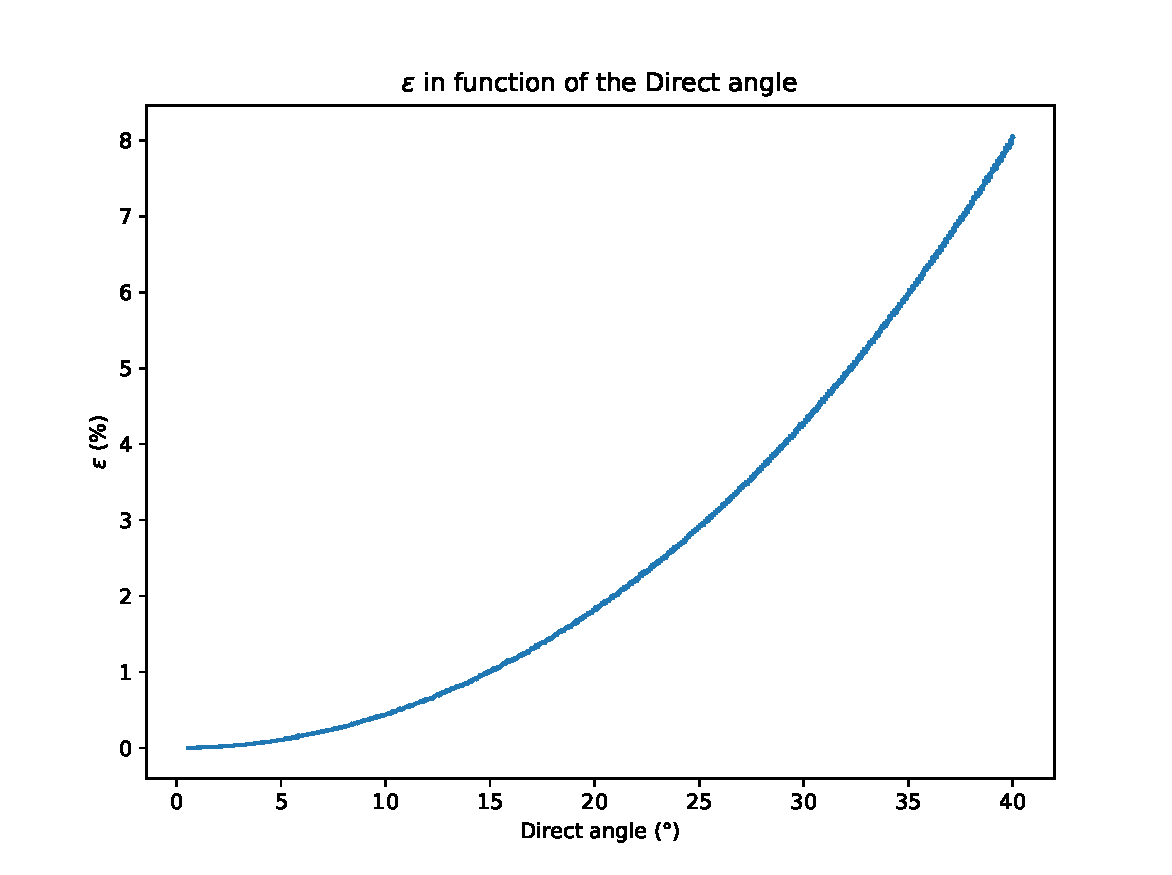
\includegraphics[width=0.7\textwidth]{EpsilonIFODirectSnell.pdf}
	\caption{epsilon IFO possible angles from channels 0-3 with refraction at the surface}
	\label{fig:EpsilonIFODirectSnell}
\end{figure}
As you can see we can now go up to 15° and still have a relative accuracy of less than 1\%!  The
only drawback of this method is that we need to assume the index of refraction
to be 1.27 at the surface of the ice, if this isn't the case in some places our
predictions won't be accurate.

\begin{figure}
  \centering
	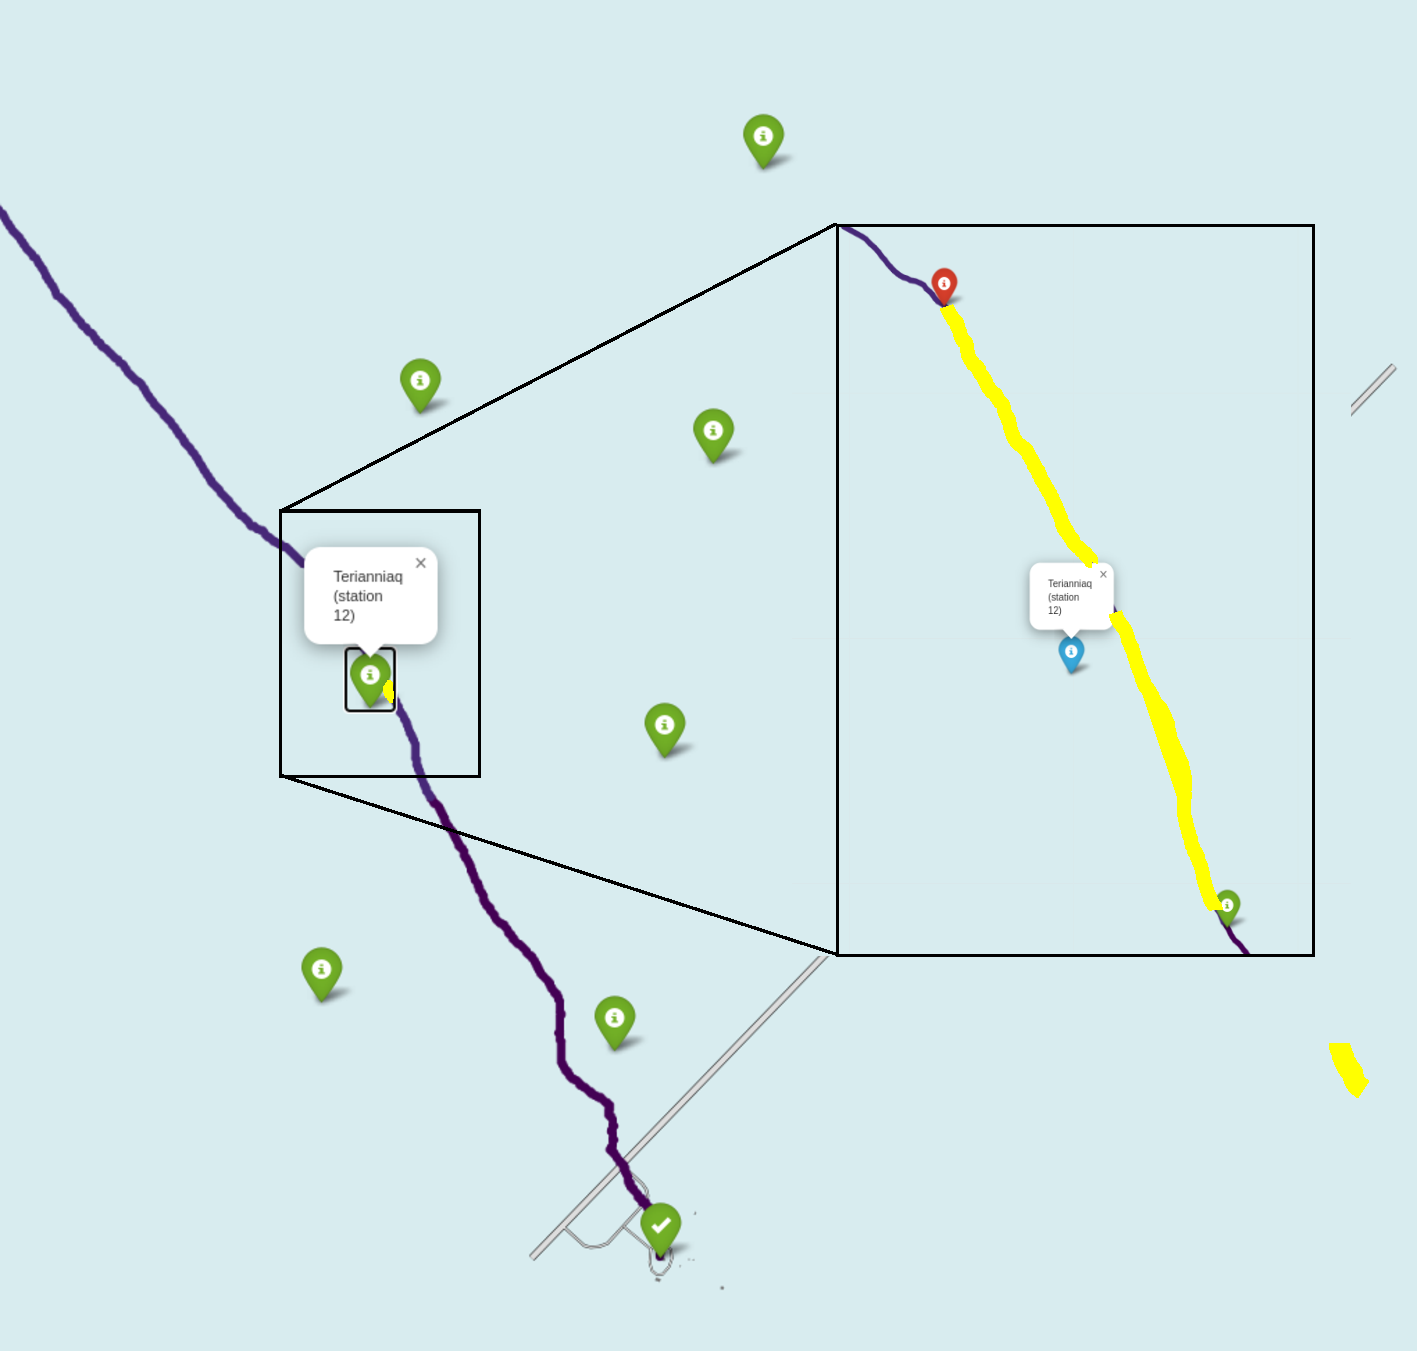
\includegraphics[width=0.7\textwidth]{BallonPathAllIllu.pdf}
  \caption{Path traced out by a weather balloon in purple released at 20/08/2022, in yellow you can see when it
  gets within 10° of detector 12.}
  \label{fig:ExampleBalloonPathCrossing12}
\end{figure}


\subsection{Influence of height on Epsilon}
In the previous sections we've assumed the height of the weather balloon to be
500m, does changing this height influence the behaviour of $\epsilon$ in some
way?  The answer is, at first surprisingly, yes. As can be seen in figure
\ref{fig:EpsWithHeight} the relative accuracy can vary with height for the same angles.
\begin{figure}
	\centering
	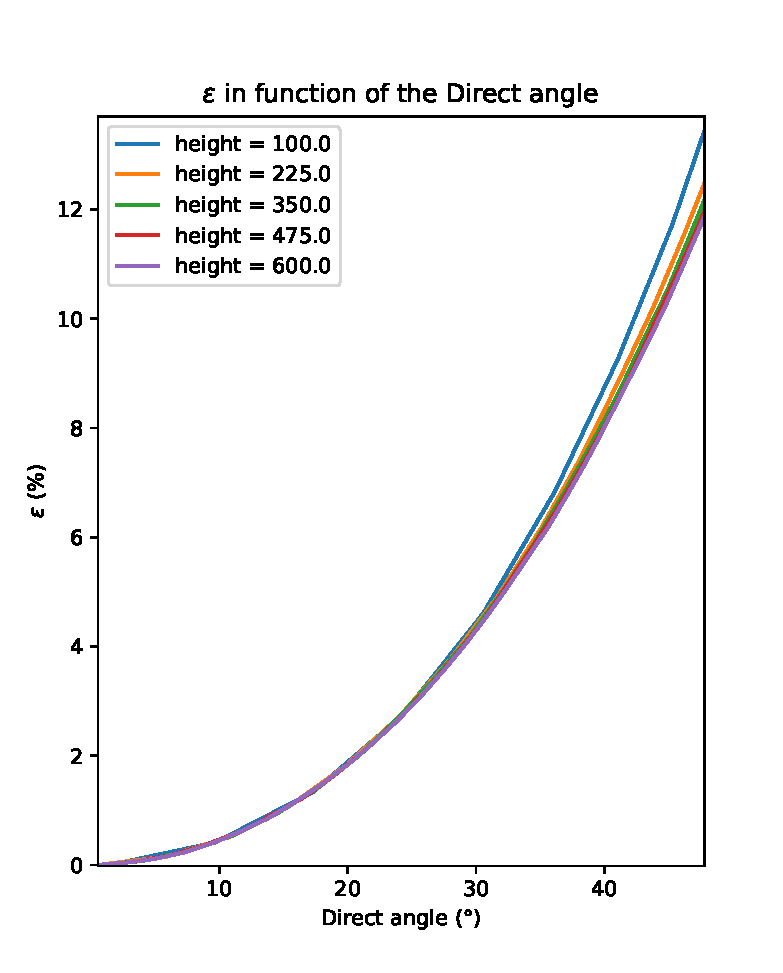
\includegraphics[height=0.4\textheight]{figures/EpsilonWithHeight.pdf}
	\caption{How varying the height influences $\epsilon$ over the same angles}
	\label{fig:EpsWithHeight}
\end{figure}
This has, as a consequence, that if we manage to get a hold on some
usable data the $\epsilon$
might still be quite large (if the height is really large).
Because of this we'll have to re-compute $\epsilon$ exactly for 
every measurement we do.
\section{Error on prediction}
Running ahead on the actual measurements, let's estimate how accurate our
predictions will be. Let's label the vertical spatial accuracy,
i.e how accurately we know the height of these channels, $\delta z$\footnote{meaning if we have a measurement $z_i$ the true value is within $z_i
\pm \delta z$ with 95\% certainty}. And the timely accuracy, or how accurate the
vpol timing characteristics are, $\delta t$. If we want to fit n, we first
minimize the summed correlation function to construct the plane wave. One
correlation function is given by 
\begin{equation}
	Correlation(\theta) := \Delta t - \Delta t' = \Delta t
	- \frac{\cos\theta \Delta z}{v}
\end{equation}
Say the minimum occurs at $Correlation(\theta) = Correlation(\theta_{min}) := \mathcal{C}$, we can then re-write 
this equation for n:
\begin{equation}
  n = \frac{c(\Delta t - \mathcal{C})}{\cos \theta_{min} \Delta z} = \frac{c}{\cos{\theta_{min}}}\left[\frac{\Delta t}{\Delta z} - \frac{\mathcal{C}}{\Delta z}\right]
\end{equation}
The $\Delta z$ is the vertical distance between two channels and thus has an error of $2\delta z$ and $\Delta t$ is the time
difference between two channels, implying an error $2\delta t$. 
Let's look at the two terms seperately (assuming the error on $\theta_{min}$ to be negligable),
the first quotient $\phi_1 := \Delta t/\Delta z$ has a variance \cite{grabe2005measurement} of
\begin{equation}
	s_{\phi_1}^2 = \frac{1}{{\Delta z}^2}s_{\Delta t}^2 - 2 \frac{{\Delta t}}{{\Delta z}^3}s_{\Delta t \Delta z} + \frac{{\Delta t}^2}{{\Delta z}^4}s_{\Delta z}^2
\end{equation}
Assuming $\Delta t$ and $\Delta z$ to be independent:
\begin{align}
	s_{\phi_1}^2 &= \frac{1}{{\Delta z}^2}s_{\Delta t}^2 + \frac{{\Delta t}^2}{{\Delta z}^4}s_{\Delta z}^2\\
	&= 4\left(\frac{1}{{\Delta z}^2}{\delta t}^2 + \frac{{\Delta t}^2}{{\Delta z}^4}{\delta z}^2\right)
\end{align}
And the second term ($\phi_2 := -\mathcal{C}/\Delta z$):
\begin{align}
	s_{\phi_2}^2 &= \frac{\mathcal{C}^2}{{\Delta z}^2}s_{\Delta t}^2\\
		     &= 4\frac{\mathcal{C}^2}{{\Delta z}^2}{\delta t}^2\\
\end{align}
Our squared variance on the index of refraction is thus (neglecting unknown systematic errors):
\begin{equation}
	\delta n^2 =: s_n^2 = 4\left(\frac{c}{\cos{\theta_{min}}}\right)^2 \left( \frac{1}{{\Delta z}^2}{\delta t}^2 + \frac{{\Delta t}^2}{{\Delta z}^4}{\delta z}^2 + 
\frac{\mathcal{C}^2}{{\Delta z}^2}{\delta t}^2\right)
\end{equation}
If we have more than 2 detectors, say N then the uncertainty on the fit can be assumed to be the
RMS of the individual uncertainties:
\begin{equation}
  \delta n =\sqrt{\sum_{i=0}^N \delta n _i^2}
\end{equation}
Let's assume $\epsilon$ to be an absolute error.  Now due to this inherent
inaccuracy, the "global" uncertainty on n also has an additional error of $\pm \epsilon(\vec{r})n$ with
$\vec{r}$ the position of the balloon.  Our final error on n is thus:
\begin{equation}
  \delta n(\vec{r})=  \epsilon(\vec{r})n + \sqrt{\sum_{i=0}^N 4\left(\frac{c}{\cos{\theta_{min}}}\right)^2 \left( \frac{1}{{\Delta z_i}^2}{\delta t}^2 + \frac{{\Delta t_i}^2}{{\Delta z_i}^4}{\delta z}^2 + 
  \frac{\mathcal{C}_i^2}{{\Delta z_i}^2}{\delta t}^2\right)}
  \label{eqn:total error}
\end{equation}
If we \textbf{assume the $\epsilon$ to overestimate the index of refraction the same way in real
life as in the simulation} however, our estimated $n$ can be corrected as
\begin{equation}
  n_{\text{corrected}} (\vec{r})= \frac{n(\vec{r})}{\epsilon(\vec{r}) + 1}
\end{equation}
and our error becomes only the second part of equation \ref{eqn:total error}.
As the error on the position of the channels is not yet fully known most of
this section mainly serves as a future reference when people continue this
work, however it can be safely assumed that the timely error will be of much
higher importance than the positional error, as we'll get to in section (???).  

The error on timing can be estimated, contrary to the positional error, from the
sampling rate, as if we have a sampling rate of e.g 3.2GHz then the antenna
will take a measurement every 
\begin{equation}
	\delta t = \frac{1}{3.2\text{GHz}} = 0.3125\text{ns}
\end{equation}
So we can predict a measurement of the index of refraction, assuming $\epsilon$
to be a correction and $\delta z \ll$, to have an error of
\begin{align}
	\delta n(\vec{r})_{\text{corrected}}&=  (1+\epsilon)\times\sqrt{\sum_{i=0}^N 4\left(\frac{c}{\cos{\theta_{min}}}\right)^2 \left( \frac{1}{{\Delta z_i}^2}{\delta t}^2 +
  \frac{\mathcal{C}_i^2}{{\Delta z_i}^2}{\delta t}^2\right) }\\
					    &=  2(1+\epsilon){\delta t} \times\sqrt{\sum_{i=0}^N \left(\frac{c}{\cos{\theta_{min}}}\right)^2 \left( \frac{1}{{\Delta z_i}^2}+
  \frac{\mathcal{C}_i^2}{{\Delta z_i}^2}\right) }\\
					    &=  2(1+\epsilon){\delta t} \times\sqrt{\sum_{i=0}^N \left(\frac{c}{\Delta z_i\cos{\theta_{min}}}\right)^2 \left(1 +
  \mathcal{C}_i^2\right)}
  \label{eqn:errorcorr}
\end{align}
And if we only consider 2 detectors (which we will in most cases) this reduces
to
\begin{equation}
	\delta n(\vec{r})_{\text{corrected}} = 2(1+\epsilon)\times c\left(\frac{\delta t}{\Delta z}\right) \times\left[\frac{\sqrt{1 +
	\mathcal{C}^2}}{\cos{\theta_{min}}}\right]
\end{equation}
Note again that $\Delta z$ is the \textbf{difference} in height between the two
detectors and $\delta t$ is the \textbf{accuracy} in timing (which gets
determined by the sample rate of the antenna).

\newpage
\section{Fitting the index: Channels 0 and 3}
Now that we know our goal to be feasible, let's analyse some data.  As we'll
start by just analysing one event, let's take a very good one for our analysis.
A close look at graph \ref{fig:EpsilonIFODirect} shows that events under 5° at
a height of 500m produce an $\epsilon$ of less than 0.22\%, implying that if we
measure n to be 1.7407 our $\epsilon$ will only be 0.0038.  A good start will
thus be finding moments when the balloon gets to within a 5\% angle, note that
$\epsilon$ is height dependent so we'll have to calculate it afterwards.  After
looping through all the balloon positional files and only outputting the $<5°$
ones we get the timeframes shown in appendix \ref{app:5Deg}.

If we search in the DESY database
\footnote{\url{https://rnog-monitor.zeuthen.desy.de/}} within the calculated
timeframes for the particular detectors where the balloon gets close enough to,
AND where the 403MHz signal coming from the Ballon is detected in the deep channels, the events of the 7th
of september stands out; at 11:28:10,  just before the $<5°$ passby between
11:28:47 and 11:28:49, the balloon gets quite close to detector 23 and shows a
clear 403MHz signal at the phased array, as shown in figure \ref{fig:freqs03}.

Now to calculate the differences in timing for this received signal, the code
we built for this is called FitN.py and stored at the repository
\href{https://github.com/arthuradriaens-code/projects-mt.git}{projects-mt}
under BaLLooN/RealData, let's go over the full code step by step:\footnote{I advise 
the people who will continue this work to pull up the code side-by-side with this 
explanation}

\subsection{Spatial data}
The first part we'll need to concern ourselves with is determining the relative
positions of everything. The balloon data file and the time when the event took
place are given, from these two both the latitudinal and longitudinal position
and the elevation of the balloon at the given time are determined. We convert
these three measurements to the ENU coordinate frame (x,y,z with respect to
refrence) and store it in the array \textit{BalloonPosition}. The next step is
to get the location of the detector, for this we first instantiate a detector
object 

\begin{mintedbox}{python}
det = NuRadioReco.detector.detector.Detector(json_file="RNO_season_2022.json")
\end{mintedbox}

The RNO season 2022 json file can be found on the official RNO-G github under
"analysis-tools", then we update the detector to the time of the event and get
the absolute position of our detector (station 23) via the
get\_absolute\_position module:

\begin{mintedbox}{python}
	stationlocation = det.get_absolute_position(station_id)
\end{mintedbox}

Where at the specific station this position is doesn't matter as we'll explains
shortly.  Now that we have both the position of our balloon and station in ENU
coordinates, let's simplify the calculations by setting the detector as the
origin.  i.e our new balloon position will be

\begin{equation}
	\textit{RelBalloon} = \textit{BalloonPosition} - \textit{StationPosition}
\end{equation}

And as we might want to plot this later, due to the cylindrical symmetry of the
ice model, we can rotate the coordinates to get rid of our y-axis. We can do
this by defining the radius:

\begin{equation}
	r := \sqrt{\textit{RelBalloon}_x^2 + \textit{RelBalloon}_y^2}
\end{equation}

and just setting this equal to $\textit{Balloon}_x$ and setting $\textit{Balloon}_y$ to
zero (equivalent to setting $\theta= 0$ in a rotation).

We don't have the position of our individual channels yet, only of the
station itself, these can however easily be obtained using the
get\_relative\_position module on our detector object, as we chose our station
to be the center of the coordinate system, these relative positions are
absolute positions of the channels in our frame of reference. Using
these it thus doesn't matter where the position of the station was defined.

\subsection{Signal analysis and initial guesses}
Now that we have our geometry, let's analyse the data for the channels 0 and 3,
the data for a particulal channel is stored in a channel object. From this
object we can get the recorded voltages with the get\_trace() module, the
recorded times with the get\_times() module, the recorded frequencies with the
get\_frequencies() and the recorded spectrum corresponding to these frequencies
with get\_frequency\_spectrum() , note that the last two do a FFT on our data.
We know that the signal sent out by the weather balloon is a sine wave with a
frequency of 403MHz; as the data is measured in nanoseconds the frequency is:
\begin{equation}
	f = 403\text{MHz} = 403\times 10^{-3} \frac{1}{\text{ns}}
\end{equation}
The recorded spectrum of both channels is given in figure \ref{fig:freqs03}, we
observe a clear spike at 0.403GHz.
\begin{figure}
	\begin{minipage}{0.49\textwidth}
		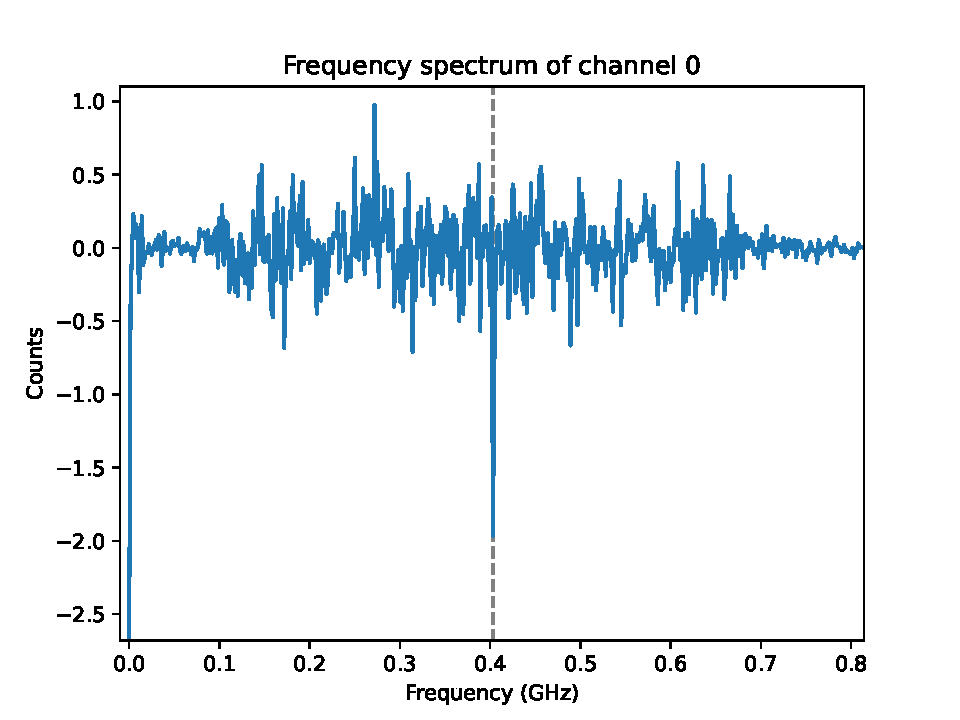
\includegraphics[width=\textwidth]{figures/23-800-0-freq.pdf}
	\end{minipage}
	\begin{minipage}{0.49\textwidth}
		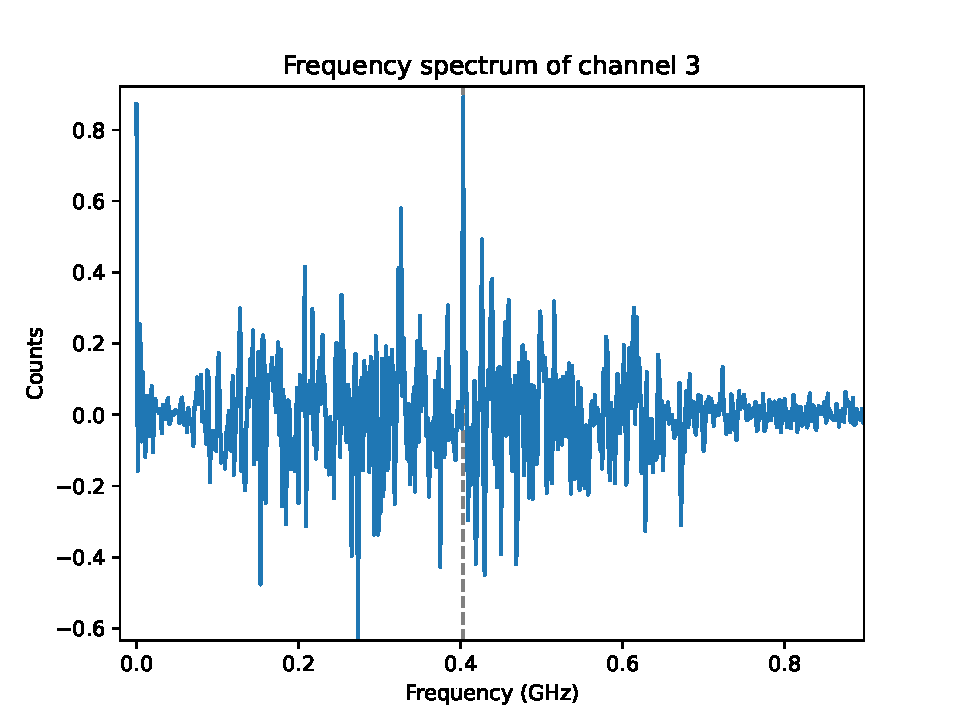
\includegraphics[width=\textwidth]{figures/23-800-3-freq.pdf}
	\end{minipage}
	\caption{recorded frequencies on detector 23 at 2022/08/29 11:18:32}
	\label{fig:freqs03}
\end{figure}
Now note that there are a bunch of peaks both below 0.15GHz and above 0.6GHz,
this is all non-physical noise as the Vpol antenna's range only goes from
0.15GHz to 0.6GHz \cite{Aguilar_2021} that's why we'll first pass this signal
trough a virtual butterworth bandpass filter.

After passing the signal through the filter we'd also like to upsample the
signal as to increase the resolution, this can be done using the resample()
module and we'll upsample towards 10GHz increasing our timely accuracy from
0.3125ns to 0.1ns.  After filtering and upsampling we have some voltage
response as shown in figure \ref{fig:VoltageAfterFilter}, we wish to find a
sine wave coming from the weather balloon in this signal.

\begin{figure}
	\centering
	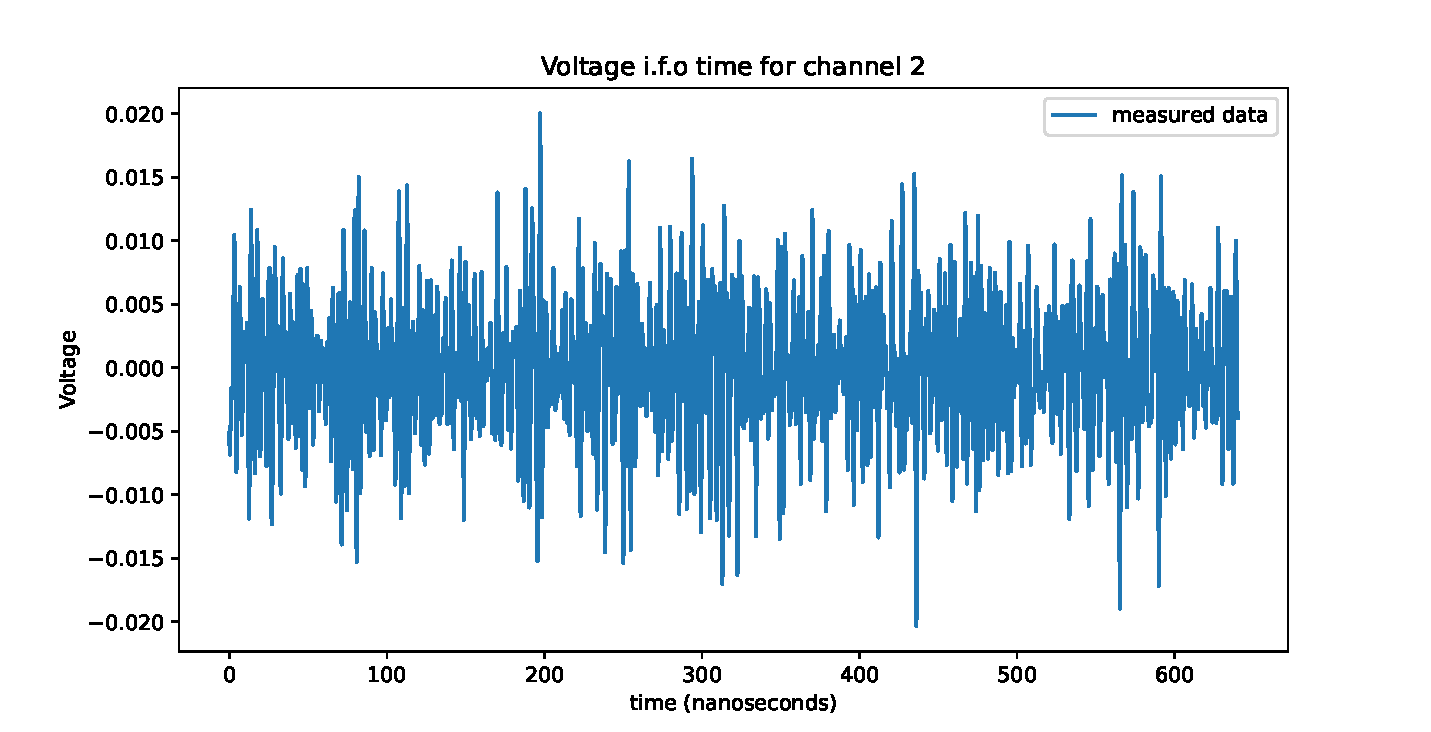
\includegraphics[width=\textwidth]{figures/VoltageAfterFilter.pdf}
	\caption{Recorded voltage i.f.o time in vpol antenna 0 after upsampling and passing through the butterworth filter}
	\label{fig:VoltageAfterFilter}
\end{figure}

To find a sine wave herein we'll radiotools' helper module get\_normalized\_xcorr
which indirectly uses scipys signal correlation function but before using that we'll
need a template to correlate with the data. The template we'll be choosing is
of course the sine function but it's important to notice that the channel has a
certain sampling rate, namely now after upsampling, 10GHz. 

Our template sine which we'll correlate to the data will also need to have this
sampling rate, meaning that it needs to be stepwise defined with spaces of
0.1ns. Next we'll also need to give the sine a certain amplitude, as we don't
have a system for finding this yet let's for now assume an amplitude $A =
0.007$ (this shouldn't impact the correlation).  Our template thus looks like
this:
\begin{equation}
	\mathcal{S} = A\cdot\sin(\omega t) 
\end{equation}
with
\begin{equation}
	\omega = 2\pi f
\end{equation}
Herein $t$ is an array going from 0 to $3/f$ as to be able to fit 3 periods
with intervals of 0.1ns.  This template gets automatically shifted by the radiotools
correlation module with steps of 0.1ns and each time the correlation with the
data gets computed as is illustrated in figure \ref{fig:SineCorrFull}.
\begin{figure}
	\centering
	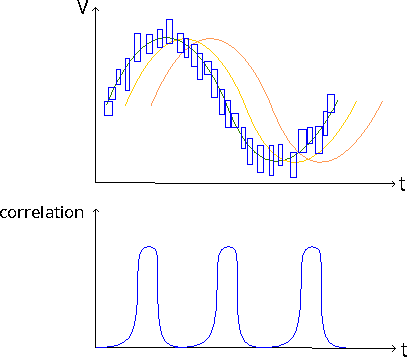
\includegraphics[width=0.8\textwidth]{figures/SineDataCorrFull.pdf}
	\caption{How correlating a sine with data leads to periodic peaks in the correlation function}
	\label{fig:SineCorrFull}
\end{figure}
In real life the data is a bit less perfect and after doing this correlation
procedure on the real data we get what's (partially) shown in figure
\ref{fig:CorrCh0}.
\begin{figure}
	\centering
	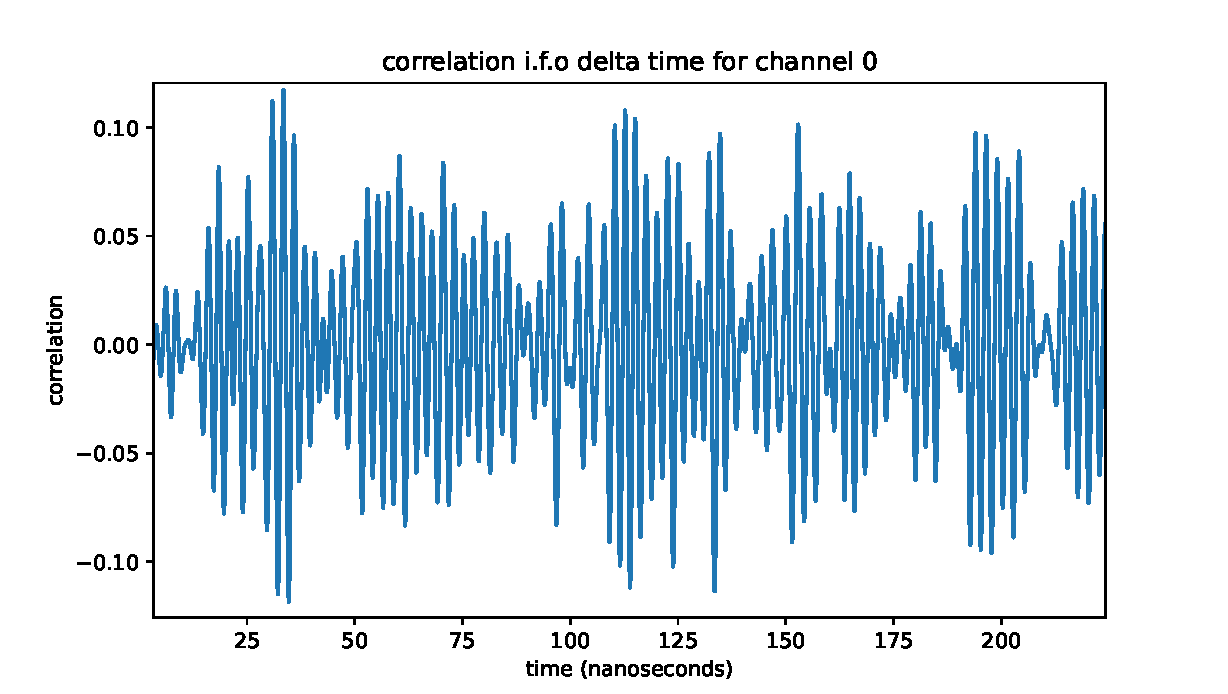
\includegraphics[width=\textwidth]{figures/CorrelationCh0.pdf}
	\caption{Zoom on the correlation i.f.o the time for channel 0}
	\label{fig:CorrCh0}
\end{figure}
Herein the peaks represent the maximal correlation, if we now do the same for
channel 3 we have two correlation functions, if we correlate these with
eachother we'll get the difference in timing between the channels.  This is
easy to comprehend after taking a look at the illustration shown in figure
\ref{fig:CorrIllu}. This cross correlation is shown in figure
\ref{fig:CrossCorr}, the negative offset is caused by accounting for cable
delay. Note that multiple peak correlations are present, to thus find out which
one is the right one we'll do a simple simulation using our modified hybrid ray
tracer from which we know what the approximate time difference is and search in
this neighbourhood.

Carrying out the full calculation we get the results which are presented below
(note that the error on the epsilon corrected n was estimated using equation \ref{eqn:errorcorr})
\begin{center}
\begin{tabular}{||c c c c c c c c||}
 \hline
 Depth (m) & Station id & channels & Run:Event & n$_\text{exp}$ & n$_\text{fit}$ & $\epsilon$ & n$_\text{corr}$\\ [0.5ex]
 \hline\hline
 -93.231 & 23 & 0\&3 & 800:1867 & 1.738 & 1.8188 & 4.6166\% & 1.739 $\pm$ 0.024 \\
 \hline
\end{tabular}
\end{center}
\begin{figure}
	\centering
	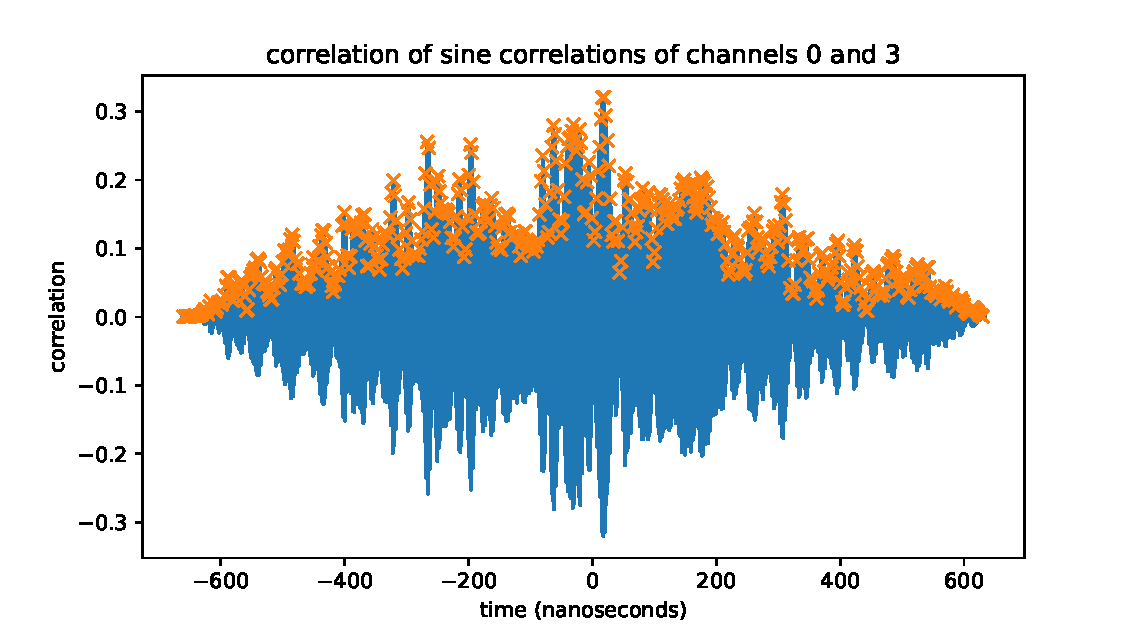
\includegraphics[width=0.9\textwidth]{figures/crosscorrelation.pdf}
	\caption{correlation of the previously, with sine, correlated dataset
	of channels 0 and 3, the orange marks indicate the peaks}
	\label{fig:CrossCorr}
\end{figure}
\begin{figure}
	\centering
	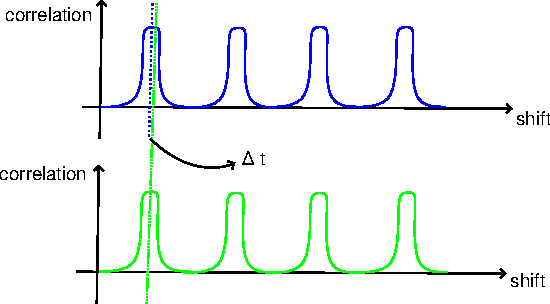
\includegraphics[width=0.9\textwidth]{figures/IlluCorr.pdf}
	\caption{Illustration of how the different correlations with sine (above
	in blue being e.g channel 0 and below in green channel 1) have a difference
in timing between the peaks which can be found from correlating the two}
	\label{fig:CorrIllu}
\end{figure}
Analogously we can use channels 0,1,2 and 3 in various combinations.
In full all possibilities are (in order of increasing depth)
\footnote{In all calculations the channel 1 had the least good
signal, as such if these calculations ever get revised try to take
this into account}\footnote{we also left out the possibility of
combinations as 0\&1\&2\&3 as the error would be quite large
and there would be no additional value but these are possible with the program}:
\begin{center}
\begin{tabular}{||c c c c c c c c||}
 \hline
 Depth (m) & Station id & channels & Run:Event & n$_\text{exp}$ & n$_\text{fit}$ & $\epsilon$ & n$_\text{corr}$\\ [0.5ex]
 \hline\hline
 -92.24 & 23 & 2\&3 & 800:1867 & 1.737 & 1.867 & 4.605\% & 1.784 $\pm$ 0.071 \\
 -92.75 & 23 & 1\&3 & 800:1867 & 1.738 & 1.800 & 4.611\% & 1.721 $\pm$ 0.036 \\
 -93.23 & 23 & 0\&3 & 800:1867 & 1.738 & 1.819 & 4.617\% & 1.739 $\pm$ 0.024 \\
 -93.24 & 23 & 1\&2 & 800:1867 & 1.738 & 1.735 & 4.616\% & 1.659 $\pm$ 0.074 \\
 -93.73 & 23 & 0\&2 & 800:1867 & 1.739 & 1.845 & 4.621\% & 1.763 $\pm$ 0.036 \\
 -94.23 & 23 & 0\&1 & 800:1867 & 1.739 & 1.858 & 4.626\% & 1.776 $\pm$ 0.073 \\
 \hline
\end{tabular}
\end{center}
Note that all the corrected fits have the exponential model's value within the margin of error.
\section{Channels 6 and 7}
A very interesting depth is between channels 5 and 7  as, looking at
the density profile shown in figure \ref{fig:DensityMeasurements}
this is where the actual density deviates the most from the models.
The event we'll be using is recorded in detector 21 at the 26th of
july 11:18:41 and falls within the $<5$° mark:
\begin{center}
\begin{tabular}{||c c c c c c c c||}
 \hline
 Depth (m) & Station id & channels & Run:Event & n$_\text{exp}$ & n$_\text{fit}$ & $\epsilon$ & n$_\text{corr}$\\ [0.5ex]
 \hline\hline
 -48.16 & 21 & 6\&7 & 1441:117 & 1.640 & 1.631 & -0.02\% & 1.631 $\pm$ 0.004 \\
 -58.38 & 21 & 5\&7 & 1441:117 & 1.674 & 1.665 & -0.23\% & 1.669 $\pm$ 0.002 \\
 -68.2 & 21 & 5\&6 & 1441:117 & 1.698 & 1.692 & 0.02\% & 1.692 $\pm$ 0.003 \\
 \hline
\end{tabular}
\end{center}
Note that none of the indices whom are found have the exponential model's index
within them.
Let's use Schytt's equation \ref{eqn:Schytt} to see where
on the density vs depth curve these values lie:
\begin{align}
	n(z) &\approx 1 + 0.78\rho/\rho_0\\
	\rho_0(n(z) - 1) &\approx 0.78\rho\\
	\frac{\rho_0}{0.78}(n(z) - 1) &\approx \rho\\
	\rho &\approx 1175.641(n(z) - 1)\frac{\text{kg}}{\text{m}^3}\\
\end{align}
The error propagation is also quite easily found:
\begin{equation}
	\delta \rho = 1175.641\delta n
\end{equation}
If we use these equations the corrected indices of refraction
correspond to the densities:
\begin{center}
\begin{tabular}{||c c||}
 \hline
 Depth (m) & $\rho_\text{corr}$\\ [0.5ex]
 \hline\hline
 -48.16 & 741.830 $\pm$ 4.703 \\
 -58.38 & 786.504 $\pm$ 2.351 \\
 -68.2 & 813.544 $\pm$ 3.527 \\
 \hline
\end{tabular}
\end{center}
If we plot this we get what's shown in figure
\ref{fig:BalloonDensity6And7}.
\begin{figure}
	\centering
	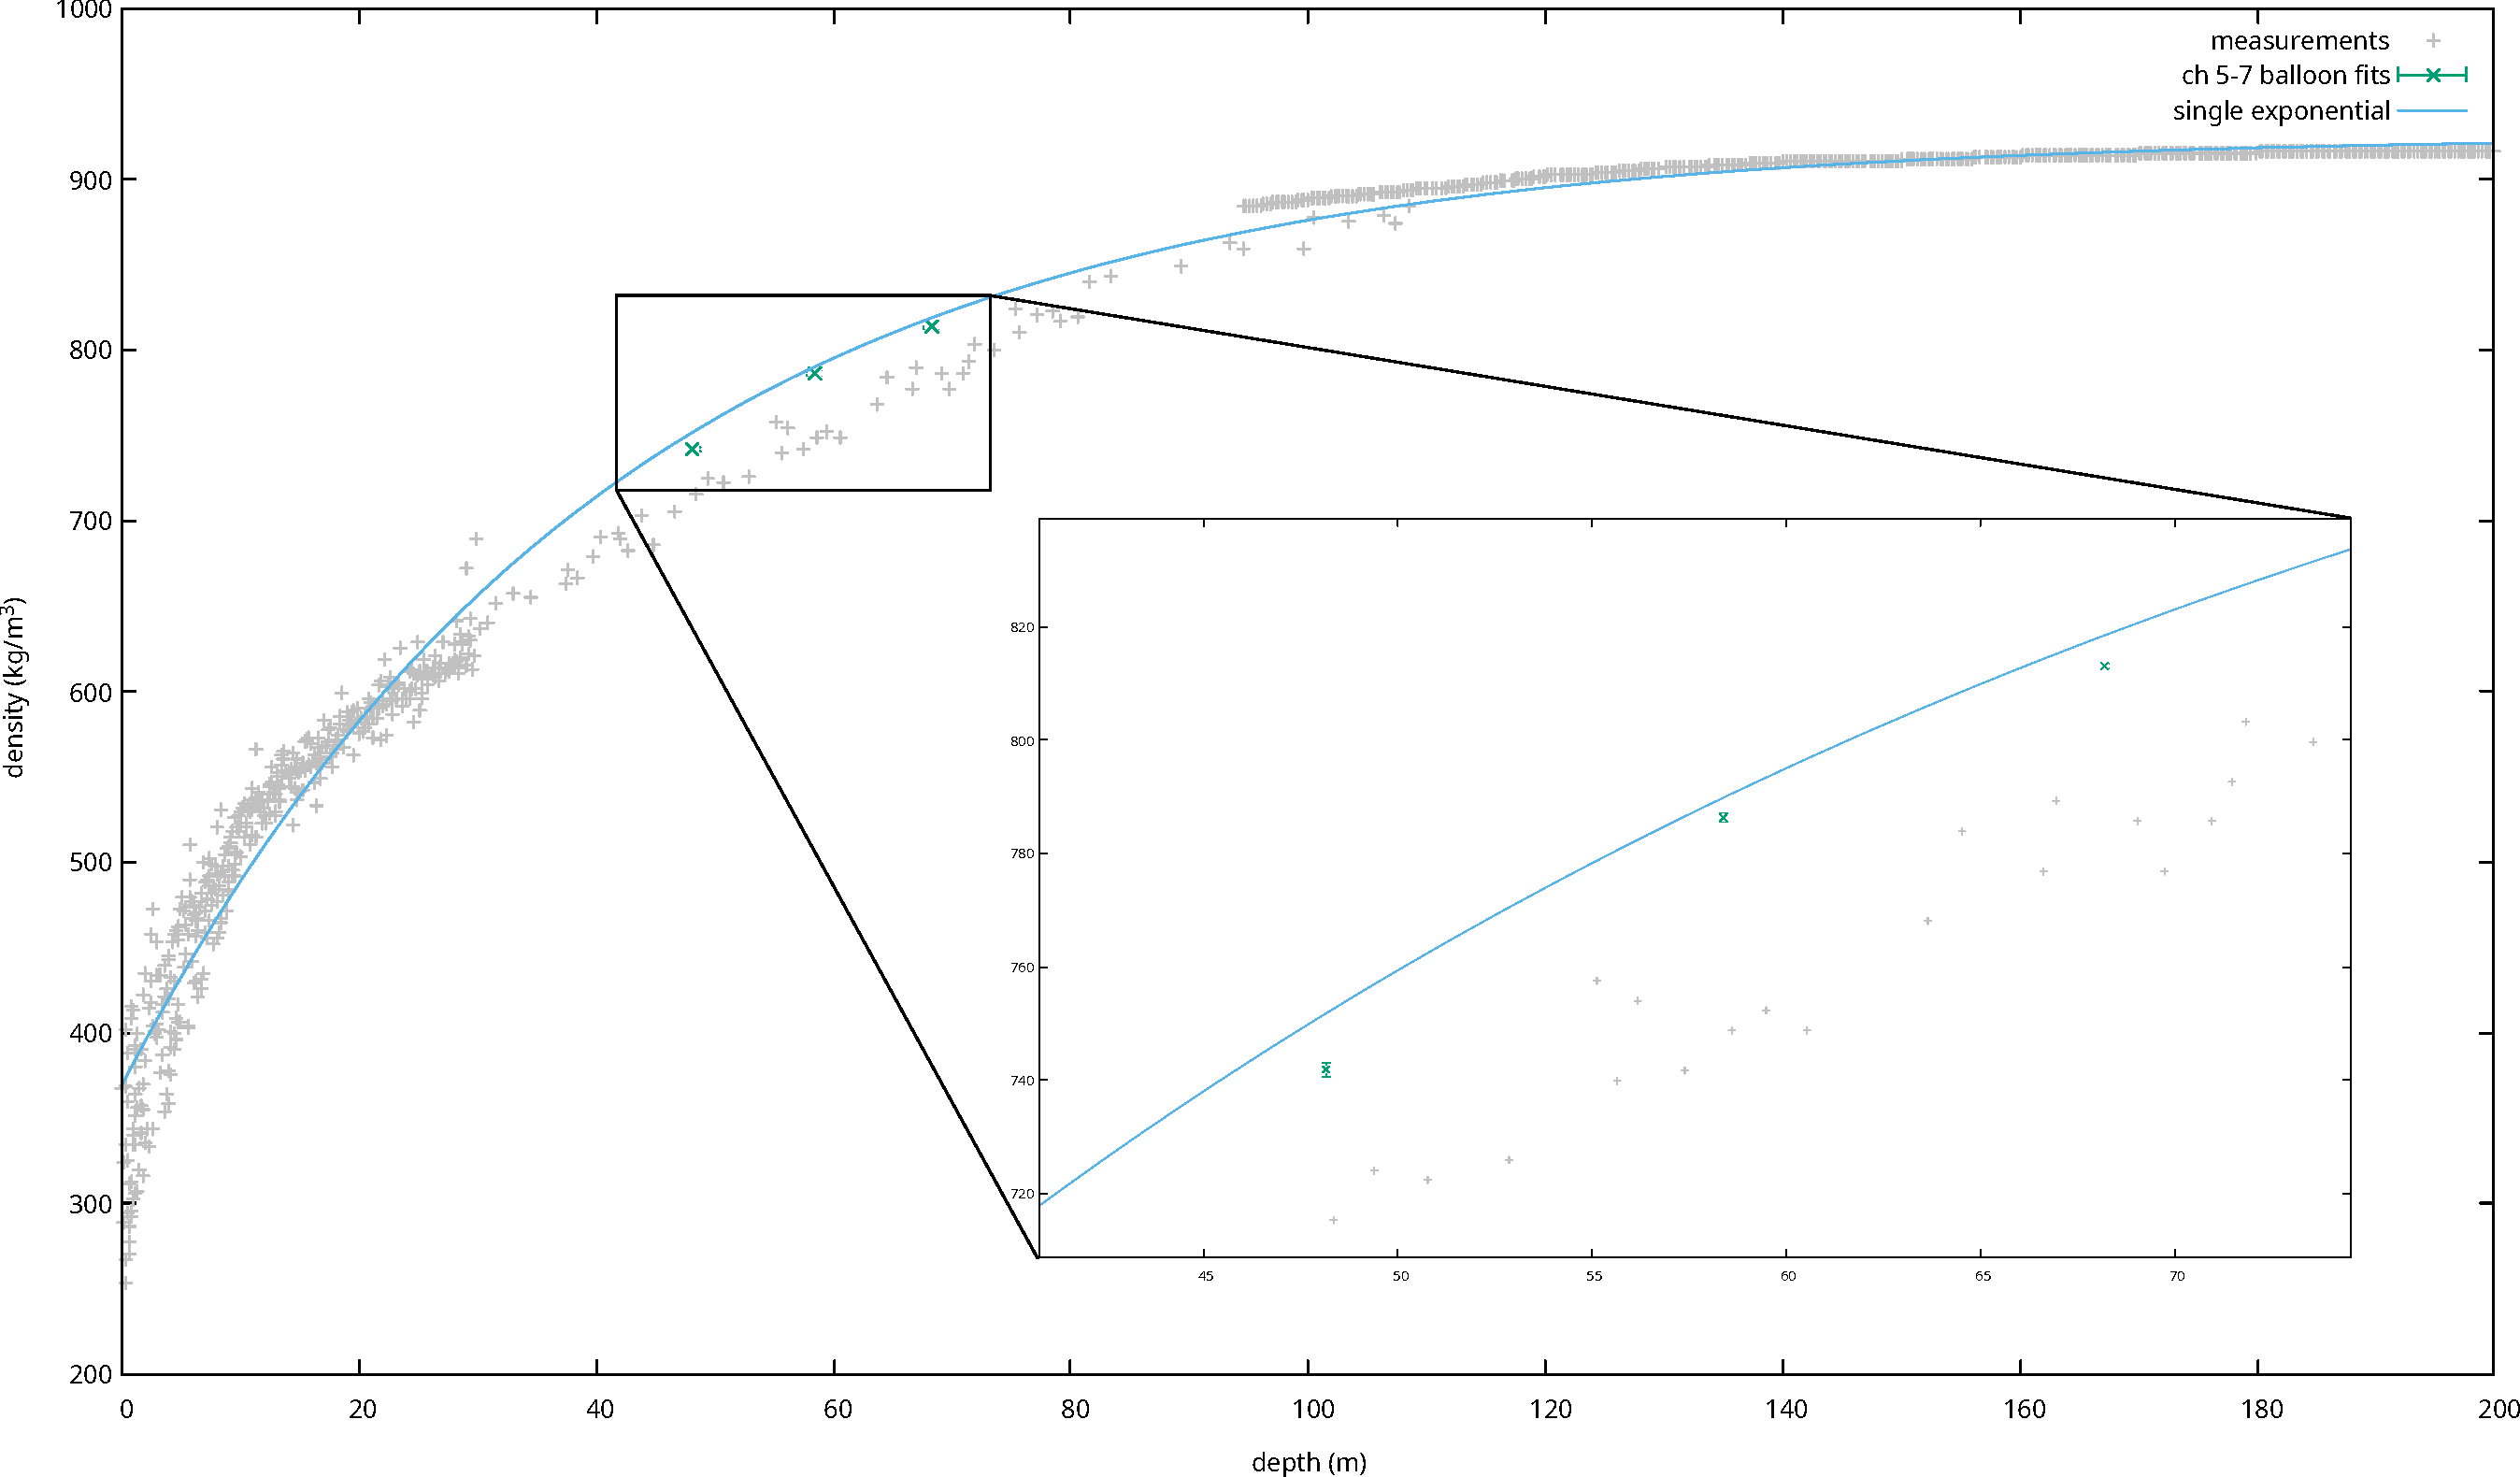
\includegraphics[width=0.9\textwidth]{DensityBalloonWithZoom.pdf}
	\caption{graph showing where the balloon data density is with
	respect to the other measurements and the exponential model}
	\label{fig:BalloonDensity6And7}
\end{figure}
Note that the calculated values neither line up with the density measurements nor with the exponential model,
but somewhere inbetween. This might be caused by one of the following reasons:
\begin{itemize}
	\item The error bar is too small
	\item Schytts law isn't fully correct
	\item The density measurements aren't correct
	\item You cannot correct the index of refraction the same way in real life
		with $\epsilon$ as in the simulation
\end{itemize}
Up until now the error on the height of the individual channels hasn't been
taken into account, let's see how big the expected error is. A fair anecdotal
estimate for the positional accuracy is 0.005m, how would this influence the
accuracy estimate? For this let's take a look at equation \ref{eqn:total
error}, for channels 6 and 7 the factor containing $\delta z$ has an order of magnitude of
($c^2$ is added to make the value dimensionless):
\begin{equation}
	c^2\frac{\Delta t_i^2}{\Delta z_i^4}\delta z^2 \sim \mathcal{O}(10^{-7}) 
\end{equation}
whilst
\begin{equation}
	c^2\frac{\delta t^2}{\Delta z_i^2} \sim \mathcal{O}(10^{-6}) 
\end{equation}
This is an order of magnitude difference, so if the error estimate is wrong it
is probably not caused by spatial inaccuracy.  The density measurements do
actually show quite a spread for nearly the same values so there might be a
problem there.  As for the Schytt's equation, wheter it is a valid
approximation or not will be descided when enough reliable data is available.
Lastly the $\epsilon$ can't be used argument also has its flaws, as if the 
density profile would scale exactly exponentially then the $\epsilon$ corrected
index would exactly fall on the exponentially expected index.
\chapter*{Conclusion}
\addcontentsline{toc}{chapter}{Conclusion}
The hybrid ray tracer developed over the course of this thesis and reported in
chapter \ref{chapter:hybrid} was a succes, not only is it more accurate than
it's predecessors but it's also faster.  The accuracy of the ray tracer also
makes it perfectly suitable for very fine precision simulations as used within
the Balloon radio wave measurements.

The use of weather balloons to estimate the index of refraction as was 
reported in \ref{chap:WB} was also 
done succesfully even though it yielded quite unexpected results, not
only were the index of refraction measured via this method deviating
from the model (with more than $2\sigma$) but also deviating from
the theoretically expected indices using the measured density and Schytts equation
\begin{equation}
	n(z) = 1+ 0.78\rho/\rho_0
\end{equation}
moreso lying somewhere inbetween. A conversion using the inverse of Schytts equation
to arrive at the density makes this especially clear as shown on figure \ref{fig:BalloonDensity6And7}.

As there are a multitude of events (as can be found in appendices
\ref{app:5Deg} and \ref{app:10Deg} but only finite time to analyse each and
every one, this code is made public
\href{https://github.com/arthuradriaens-code/projects-mt.git}{here} as to make
it easy to improve on this work.  Especially interesting might be events where
$\epsilon$ is negligable (the balloon is really close) at the phased array and
as such is the plane wave reconstruction a near perfect representation of the
actual wave.
\section*{Proposal of improved measurements}
As this method seems to be a viable way of measuring the index of refraction,
it might be a good idea to have a more controllable radio wave source fly
closer to the detectors to make more accurate measurements, e.g an
autonomous\footnote{as to not have it need a radio controller, causing RF
interference and also as autonomous GNSS positioning are always more
accurate than humans} drone with an antenna strapped to it.  Assuming Schytt's
equation to hold completely, ideally we'd like data inbetween the depths of
20-100m as this is where the biggest discrepencies might be observed between
the single exponential model and the measured density data as is depicted on
figure \ref{fig:DensityMeasurements} 

\appendix
\chapter{List of abbreviations}
\begin{itemize}
\item \textbf{AM}: \textbf{A}mplitude \textbf{M}odulated
\item \textbf{CMB}: \textbf{C}osmic \textbf{M}icrowave \textbf{B}ackground
\item \textbf{DAQ}: \textbf{D}ata \textbf{AQ}uisition system
\item \textbf{DnR}: \textbf{D}irect a\textbf{N}d \textbf{R}efracted
\item \textbf{FFT} \textbf{F}ast \textbf{F}ourrier \textbf{T}ransform
\item \textbf{GRBs}: \textbf{G}amma-\textbf{R}ay \textbf{B}ursts
\item \textbf{RADIANT}: \textbf{RA}dio \textbf{DI}gitizer and \textbf{A}uxiliary \textbf{N}eutrino \textbf{T}rigger
\item \textbf{RNO-G}: \textbf{R}adio \textbf{N}eutrino \textbf{O}bservatory in \textbf{G}reenland
\item \textbf{RF}: \textbf{R}adio \textbf{F}requency
\item \textbf{UHE}: \textbf{U}ltra \textbf{H}igh \textbf{E}nergy 
\end{itemize}
\chapter{Balloon passbys under 5°\\ in the summer of 2022}
\label{app:5Deg}
\csvautotabular{tables/EventsBelow5DegPart1.csv}
\csvautotabular{tables/EventsBelow5DegPart2.csv}
\csvautotabular{tables/EventsBelow5DegPart3.csv}
\chapter{Balloon passbys under 10°\\ in the summer of 2022}
\label{app:10Deg}
\begin{table}[h!]
\csvautotabular{tables/EventsBelow10DegPart5.csv}
\end{table}
\begin{table}
\csvautotabular{tables/EventsBelow10DegPart1.csv}
\end{table}
\begin{table}
\csvautotabular{tables/EventsBelow10DegPart2.csv}
\end{table}
\begin{table}
\csvautotabular{tables/EventsBelow10DegPart3.csv}
\end{table}
\begin{table}
\csvautotabular{tables/EventsBelow10DegPart4.csv}
\end{table}

% =====================================================================
% End matter
% =====================================================================
\newpage
%----------------------------------------------------------------------------------------
%	REFERENCE LIST
%----------------------------------------------------------------------------------------
\bibliography{sources}
\bibliographystyle{plain}

\end{document}
